\documentclass[12pt,a4paper]{report}

% Paquetes
\usepackage[utf8]{inputenc}
\usepackage[spanish]{babel}
\usepackage{graphicx}
\usepackage{amsmath}
\usepackage{hyperref}
\usepackage{geometry}
\usepackage{float}
\usepackage{caption}
\usepackage{booktabs}
\usepackage{multirow}
\usepackage{listings}
\usepackage{xcolor}
\usepackage[ruled,vlined,linesnumbered]{algorithm2e}
\usepackage[backend=biber, style=apa]{biblatex}
\addbibresource{referencias.bib}  % ajusta el nombre a tu archivo .bib
\usepackage{tikz}
\usetikzlibrary{shapes.geometric, arrows.meta, positioning}
\usepackage{titlesec}
\titleformat{\chapter}[hang]{\normalfont\huge\bfseries}{\thechapter.}{20pt}{\huge}

% Configuración de márgenes
\geometry{left=2.5cm, right=2.5cm, top=3cm, bottom=3cm}
\hypersetup{colorlinks=true, linkcolor=blue, citecolor=blue, urlcolor=blue}
\setlength{\parskip}{0.4em}
% Configuración de código
\definecolor{codegreen}{rgb}{0,0.6,0}
\definecolor{codegray}{rgb}{0.5,0.5,0.5}
\definecolor{codepurple}{rgb}{0.58,0,0.82}
\definecolor{backcolour}{rgb}{0.95,0.95,0.92}

\lstdefinestyle{mystyle}{
    backgroundcolor=\color{backcolour},   
    commentstyle=\color{codegreen},
    keywordstyle=\color{magenta},
    numberstyle=\tiny\color{codegray},
    stringstyle=\color{codepurple},
    basicstyle=\ttfamily\footnotesize,
    breakatwhitespace=false,         
    breaklines=true,                 
    captionpos=b,                    
    keepspaces=true,                 
    numbers=left,                    
    numbersep=5pt,                  
    showspaces=false,                
    showstringspaces=false,
    showtabs=false,                  
    tabsize=2,
    literate={á}{{\'a}}1 {é}{{\'e}}1 {í}{{\'i}}1 {ó}{{\'o}}1 {ú}{{\'u}}1 {ñ}{{\~n}}1 {Á}{{\'A}}1 {É}{{\'E}}1 {Í}{{\'I}}1 {Ó}{{\'O}}1 {Ú}{{\'U}}1 {Ñ}{{\~N}}1
}
\lstset{style=mystyle}

\begin{document}

% ========================================================================
% PORTADA
% ========================================================================
\begin{titlepage}
    \centering
    
    % IMAGEN (El Escudo)
    
\includegraphics[width=0.4\textwidth]{Fotos/Escudo-UM-2023-sello.jpg}
    \vspace{0.5cm}
    
    % UNIVERSIDAD
    {\scshape\LARGE Universidad de Murcia \par}
    \vspace{0.5cm}
    {\scshape\Large Facultad de Informática \par}
    \vspace{1.5cm}
    
    % TÍTULO
    \rule{\linewidth}{0.5mm} \\[0.4cm] 
    {\huge\bfseries App de trading automático con modelos computacionales \par}
    \vspace{0.2cm}
    {\Large\bfseries Trabajo de Fin de Grado \par}
    \rule{\linewidth}{0.5mm} \\[1cm]
    
    % AUTOR Y TUTOR
    \begin{flushright}
        \large
        \emph{Autor:} \\
        \textbf{Alejandro López López} \\
        Grado en Ingeniería Informática \\[1cm]
        
        \emph{Tutores:} \\
        \textbf{Dra. Doña Raquel Martínez España}\\
        \textbf{Dr. D. José Tomás Palma Mendez}\\
    \end{flushright}
    
    \vfill
    
\end{titlepage}

\thispagestyle{empty}
\newpage

% ÍNDICES
\tableofcontents
\newpage
\listoffigures
\addcontentsline{toc}{chapter}{Índice de figuras}
\newpage
\listoftables
\addcontentsline{toc}{chapter}{Índice de tablas}
\newpage

% CAPÍTULOS
\chapter{Resumen}
\label{chap:resumen}
Texto comentado
% Este Trabajo de Fin de Grado presenta el desarrollo de una plataforma de trading algorítmico orientada a estudiantes. El objetivo principal es proporcionar un entorno controlado y seguro donde los usuarios puedan experimentar con estrategias de inversión utilizando datos reales del mercado de criptomonedas, sin exponer capital real al riesgo financiero.

% La arquitectura del sistema es híbrida y modular, integrando un orquestador Java robusto (Spring Boot) para la gestión contable y el ciclo de vida de las operaciones, con un motor de cálculo en Python. Esta dualidad permite ejecutar simulaciones precisas (Backtesting) y operativa en tiempo real simulada (Paper Trading). Una característica de la plataforma es que tanto por backtesting como por paper trading, pueden ver los resultados y las operaciones realizadas. También es posible agrupar los datos historicos de varias monedas para luego entrenar modelos de Inteligencia Artificial, ya sea con indicadores basicos o con los resultados de las estrategias.

% \vspace{0.5cm}
% \noindent \textbf{Palabras clave:} Trading Educativo, Criptomonedas, Spring Boot, Python, Inteligencia Artificial, Backtesting.

% --- Abstract ---
\newpage
\chapter{Extended Abstract}
\label{chap:abstract}

Texto comentado
% This Final Degree Project presents the development of an algorithmic trading platform tailored for students. The primary objective is to provide a controlled and secure environment where users can experiment with investment strategies using real-world cryptocurrency market data, without exposing actual capital to financial risk.

% The system architecture is hybrid and modular, integrating a robust Java orchestrator (Spring Boot) for accounting management and operational lifecycle, with a Python calculation engine. This duality enables the execution of accurate simulations (Backtesting) and simulated real-time trading (Paper Trading). A key feature of the platform is that it provides detailed visibility into the results and operations performed in both modes. Furthermore, the system allows for the aggregation of historical data from multiple cryptocurrencies to train Artificial Intelligence models, utilizing either basic technical indicators or the specific results generated by the strategies.

% \vspace{0.5cm}
% \noindent \textbf{Keywords:} Educational Trading, Cryptocurrencies, Spring Boot, Python, Artificial Intelligence, Backtesting.

 % Se deja vacío intencionalmente
\newpage
\chapter{Introducción}
\label{chap:introduccion}

Las criptomonedas han revolucionado el panorama financiero, ofreciendo nuevas oportunidades de inversión y especulación a corto, mediano y largo plazo \parencite{baur_bitcoin_2017}. Sin embargo, la volatilidad inherente a estos activos y la complejidad de los mercados digitales presentan desafíos significativos para los inversores \parencite{katsiampa_volatility_2017}. A diferencia de los mercados bursátiles tradicionales, los mercados de criptomonedas operan de forma ininterrumpida, los siete días de la semana, a escala global y sin un regulador centralizado. Esta naturaleza descentralizada, sumada a la velocidad con la que los precios pueden variar en cuestión de minutos, hace que la toma de decisiones humana por sí sola sea insuficiente para competir con los sistemas automatizados que dominan actualmente estos mercados. Mientras que en la bolsa tradicional un inversor minorista podía analizar la situación con calma durante el horario de mercado, en el ecosistema cripto esta ventana se ha cerrado: el mercado no duerme, las oportunidades son efímeras y los errores de juicio tienen consecuencias inmediatas. A esto se añade que la barrera de entrada se ha reducido drásticamente gracias a plataformas de fácil acceso, lo que ha atraído a millones de inversores sin experiencia previa que se enfrentan a un entorno hostil sin las herramientas ni los conocimientos necesarios para navegarlo de forma racional.

La necesidad de este proyecto radica, en primer lugar, en la dificultad inherente de los usuarios para reaccionar en tiempo real ante estas rápidas fluctuaciones del mercado. A esto se suma una carencia generalizada de educación financiera básica, especialmente entre los jóvenes y los inversores minoristas \parencite{lusardi_economic_2014}. En la actualidad, resulta complejo iniciarse en el mundo de la inversión de forma segura y sin arriesgar capital real. Este problema se ve agravado por la sobreabundancia de ruido mediático y atención pública desmedida en torno a estos activos. Como demuestra la literatura reciente, esto fomenta expectativas irreales que empujan a los usuarios inexpertos (especialmente a los más jóvenes) a operar de forma altamente especulativa y con excesiva frecuencia, lo que habitualmente desemboca en menores rendimientos y la pérdida paulatina de sus ahorros \parencite{hasso_who_2019}. Por otro lado, el trading algorítmico ofrece la gran ventaja de eliminar el sesgo emocional de las decisiones de inversión, aportando una mayor disciplina y consistencia matemática en la ejecución de las estrategias \parencite{chan_algorithmic_2013}. Sin embargo, la alta barrera de entrada, derivada de la profunda complejidad técnica y la falta de acceso a herramientas de simulación adecuadas, dificulta enormemente el aprendizaje \parencite{treleaven_algorithmic_2013}.

En este contexto, las \textit{estrategias de trading} constituyen la respuesta natural a estos problemas. Una estrategia no es más que un conjunto de reglas objetivas y reproducibles basadas en indicadores técnicos como la media móvil, el RSI o el MACD— que determinan de forma autónoma cuándo comprar y cuándo vender un activo, eliminando así la subjetividad y la reacción emocional del inversor humano \parencite{murphy_technical_1999}. El valor real de las estrategias, sin embargo, no reside únicamente en su ejecución en tiempo real, sino en la posibilidad de validarlas previamente sobre datos históricos mediante el \textit{backtesting}: un proceso que permite medir su rendimiento pasado antes de comprometer capital real. Esta capacidad de experimentación controlada resulta fundamental para el aprendizaje, pues permite al inversor iterar sobre sus hipótesis, detectar sus errores y desarrollar un criterio crítico sin consecuencias económicas. A pesar de ello, el diseño, la implementación y la validación de estas estrategias sigue siendo una tarea reservada a perfiles con conocimientos avanzados de programación y matemáticas financieras, lo que excluye a la inmensa mayoría de los inversores interesados en adoptarlas.

Para abordar esta problemática, este proyecto se centra en el desarrollo de una plataforma de trading algorítmico orientada a reducir esta brecha técnica, democratizando el acceso al trading cuantitativo. El sistema proporciona a los estudiantes un entorno de simulación seguro (\textit{Paper Trading}) donde pueden experimentar, aprender de sus errores y validar sus hipótesis sin riesgo financiero. Además, la plataforma centraliza la exportación de resultados en formato CSV para su auditoría. Asimismo, para aquellos con un perfil más técnico, el sistema proporciona una base sólida para la recopilación de datos históricos de múltiples monedas y la aplicación práctica de modelos de Inteligencia Artificial, ya sea entrenando algoritmos con indicadores básicos o retroalimentándolos con los resultados de las estrategias del usuario.

Finalmente, para facilitar la curva de aprendizaje, el formato de las estrategias se basa en el estándar utilizado por \textit{Freqtrade} \parencite{freqtrade_development_team_freqtrade_2023}, una plataforma de código abierto escrita en Python. Este formato permite a los usuarios definir sus propias reglas operativas de forma intuitiva. Las estrategias se implementan como scripts que interactúan con el motor de cálculo para recibir datos de mercado, procesar señales y enviar órdenes, permitiendo al estudiante centrarse puramente en la lógica financiera mientras el sistema gestiona la complejidad subyacente.

\newpage
\chapter{Objetivos}

\label{chap:objetivos}

\section{Objetivo General}
El objetivo principal de este Trabajo de Fin de Grado es desarrollar una plataforma de trading algorítmico y simulación (backtesting) para el mercado de criptomonedas, capaz de integrar dinámicamente indicadores técnicos personalizados y modelos de Inteligencia Artificial para la predicción direccional del precio.

\section{Objetivos Específicos}

Para alcanzar el objetivo general propuesto, se establecen los siguientes objetivos específicos, alineados con las fases del ciclo de vida del desarrollo de software: Estos objetivos se derivan de la problemática descrita en el Capítulo \ref{chap:introduccion} y estructuran la validación técnica posterior en los Capítulos \ref{chap:metodologia}, \ref{chap:desarrollo} y \ref{chap:conclusiones}.

\begin{itemize}
    \item \textbf{Estudiar} el estado del arte del trading cuantitativo, analizando la formulación matemática de los indicadores técnicos básicos y los paradigmas actuales de \textit{Machine Learning} aplicados a series temporales financieras.
    
    \item \textbf{Analizar} los requisitos funcionales y no funcionales necesarios para la construcción de un sistema financiero de alta concurrencia.
    
    \item \textbf{Diseñar} una arquitectura de software modular y distribuida que desacople la lógica de orquestación transaccional del motor de entrenamiento e inferencia estadística.
    
    \item \textbf{Desarrollar} un motor de ingesta y sincronización de datos de mercado automatizado capaz de procesar, limpiar y almacenar masivamente velas transaccionales (\textit{candlesticks}) desde fuentes externas (APIs).
    
    \item \textbf{Implementar} un pipeline de Inteligencia Artificial paramétrico que permita al usuario configurar, entrenar y evaluar múltiples algoritmos predictivos inyectando hiperparámetros de forma dinámica.
    
    \item \textbf{Evaluar y validar} la robustez y efectividad de la plataforma mediante la ejecución de simulaciones históricas (\textit{backtesting}), analizando métricas de rendimiento computacional y financiero (tasa de acierto, factor de beneficio y reducción máxima o \textit{drawdown}).
\end{itemize}

\newpage
\chapter{Estado del Arte}
\label{chap:estado_del_arte}

El desarrollo de sistemas de trading algorítmico ha experimentado una transformación radical en la última década, pasando de la ejecución de simples reglas estáticas a la integración de modelos complejos de Inteligencia Artificial (IA) \parencite{treleaven_algorithmic_2013}. En esta sección se analizan las tecnologías, paradigmas y algoritmos que conforman el estado actual de la predicción de mercados financieros y las arquitecturas de software de trading. El recorrido de este capítulo sigue la misma lógica del sistema desarrollado: primero se sitúa la evolución del trading algorítmico, después cómo se construyen las variables de entrada del módulo predictivo, a continuación se revisan las familias de modelos que permiten formular la predicción direccional y, finalmente, se analiza la arquitectura software necesaria para integrar cálculo analítico, persistencia y ejecución.

\section{Evolución del Trading Algorítmico}

El trading algorítmico consiste en el uso de programas informáticos para introducir órdenes de compra y venta en los mercados financieros con base en un conjunto de reglas predefinidas \parencite{chan_algorithmic_2013}. Históricamente, estos sistemas se basaban en el Análisis Técnico tradicional, utilizando indicadores matemáticos retrospectivos \parencite{murphy_technical_1999}. Sin embargo, la Hipótesis de los Mercados Eficientes \parencite{fama_efficient_1970} sugiere que los precios de los activos reflejan toda la información disponible, lo que hace que los métodos puramente lineales sean insuficientes en mercados de alta liquidez como el de las criptomonedas \parencite{katsiampa_volatility_2017}. Esto ha provocado la migración hacia el análisis cuantitativo y el modelado no lineal mediante aprendizaje automático \parencite{lopez_de_prado_advances_2018}.

Esta evolución explica que, antes de discutir algoritmos concretos, resulte necesario revisar cómo se construyen las variables con las que esos modelos operan. En un sistema como el desarrollado en este trabajo, la predicción no se plantea sobre velas OHLCV en bruto, sino sobre indicadores que representan la tendencia, momento y volatilidad.

\section{Datos y Modelos Predictivos}

A pesar del auge de la IA, los indicadores técnicos clásicos siguen siendo la base fundamental para la fase de extracción de características \parencite{lopez_de_prado_advances_2018}. La literatura actual demuestra que la combinación de indicadores de tendencia (como la Media Móvil Exponencial, EMA), de momento (como el Relative Strength Index, RSI) y de volatilidad (como el Average True Range, ATR) proporcionan a los modelos predictivos el contexto necesario para identificar regímenes de mercado \parencite[Caps. 9, 10 y 16]{murphy_technical_1999}. El preprocesamiento de estos datos en ventanas temporales escalonadas es vital para reducir el ruido del precio \parencite{chan_algorithmic_2013,lopez_de_prado_advances_2018}.

En este proyecto, el módulo predictivo se apoya precisamente en un conjunto de variables calculables y comparables. Una vez construido ese espacio de características, el problema pasa a ser decidir qué familias de modelos supervisados resultan más adecuadas para predecir la dirección de la siguiente vela. La predicción del movimiento direccional del precio (clasificación: sube, baja o lateral) es uno de los problemas más complejos en el ámbito del aprendizaje automático, debido a la baja relación señal-ruido de los mercados financieros \parencite{fama_efficient_1970}. Actualmente, la industria se apoya en las siguientes familias de algoritmos:

\begin{description}
    \item[\normalfont\textbf{Modelos de Ensamblado basados en Árboles.}] Los métodos de ensamblado dominan las competiciones de ciencia de datos tabulares financieras \parencite{lopez_de_prado_advances_2018}. \textbf{Random Forest} actúa como el estándar de la industria para establecer referencias robustas gracias a su resistencia al sobreajuste, lograda al combinar múltiples árboles de decisión independientes \parencite{breiman_random_2001}. Por su parte, los métodos de \textbf{Gradient Boosting} como XGBoost \parencite{chen_xgboost_2016} y LightGBM \parencite{ke_lightgbm_2017} destacan por su alta precisión en conjuntos de datos tabulares: XGBoost incorpora técnicas de regularización que reducen el sobreajuste y mejoran la selección de variables relevantes \parencite{chen_xgboost_2016}, mientras que LightGBM ofrece un entrenamiento más rápido y eficiente en memoria \parencite{ke_lightgbm_2017}, siendo el algoritmo preferido para procesar grandes volúmenes de datos históricos.

    \item[\normalfont\textbf{Máquinas de Vectores de Soporte (SVM).}] En su formulación matemática, las SVM transforman los datos de entrada a un espacio de mayor dimensión mediante funciones núcleo para encontrar un hiperplano de separación óptimo \parencite{cortes_support-vector_1995}. Aplicado al dominio financiero, aunque estas técnicas resultan computacionalmente costosas al procesar conjuntos de datos masivos, siguen siendo una herramienta valiosa para identificar cambios de tendencia macroeconómicos cuando se utilizan con variables muy refinadas \parencite{treleaven_algorithmic_2013,pedregosa_scikit_2011}.

    \item[\normalfont\textbf{Redes Neuronales y Aprendizaje Profundo.}] Las redes neuronales profundas han demostrado una capacidad excepcional para aprender representaciones no lineales complejas en datos financieros \parencite{goodfellow_deep_2016}. Cuando el problema se formula como clasificación direccional sobre un conjunto de indicadores técnicos precalculados, las arquitecturas densas totalmente conectadas resultan la elección natural: el modelo recibe los indicadores como entrada y predice la dirección de la siguiente vela \parencite{goodfellow_deep_2016}. La arquitectura típica combina capas de neuronas con funciones de activación no lineales, capas de regularización para reducir el sobreajuste y una capa de salida para clasificación multiclase. Su principal ventaja sobre los modelos de ensamblado radica en la capacidad de gestionar interacciones no lineales de alto orden entre indicadores \parencite{goodfellow_deep_2016}; sin embargo, su mayor tendencia al sobreajuste en conjuntos de datos reducidos y su coste computacional de entrenamiento los convierten en una herramienta complementaria a los métodos basados en árboles \parencite{lopez_de_prado_advances_2018}.
\end{description}

\section{Arquitecturas de Software para Sistemas de Trading}

Una vez fijados el tipo de variables y las familias de modelos predictivos, la cuestión deja de ser solo algorítmica y pasa a ser también de integración: cómo combinar entrenamiento, inferencia, ingesta de datos y ejecución transaccional sin mezclar responsabilidades. Ese es el contexto en el que la arquitectura software adquiere relevancia para este trabajo.

El ecosistema del desarrollo de bots de trading requiere una arquitectura distribuida que soporte alta concurrencia y baja latencia \parencite{treleaven_algorithmic_2013}. El estado del arte en ingeniería de software financiera divide estas soluciones en dos capas \parencite{richards_software_2022}:

\begin{enumerate}
    \item \textbf{Capa Transaccional y de Orquestación:} Generalmente desarrollada en lenguajes fuertemente tipados y compilados orientados a concurrencia, como Java con entornos como Spring Boot \parencite{pivotal_springboot_2024} o C++. Esta capa gestiona el enrutamiento de red, la persistencia masiva en bases de datos (inserciones masivas para series temporales) \parencite{kimball_data_2004} y la ingesta de datos en tiempo real \parencite{richards_software_2022}.

    \item \textbf{Capa Analítica (Inferencia y Entrenamiento):} Implementada casi en su totalidad en Python \parencite{hilpisch_python_2018} debido a su ecosistema superior en ciencia de datos.
\end{enumerate}

Dos de los problemas más comunes y críticos en este tipo de arquitecturas son la comunicación entre capas y la configuración de los modelos predictivos. Por un lado, la comunicación entre procesos (IPC) representa uno de los mayores desafíos técnicos \parencite{furuhashi_msgpack_2013}: las soluciones actuales optan por colas de mensajes, servicios web o comunicación directa mediante tuberías y entrada/salida estándar \parencite{treleaven_algorithmic_2013,newman_building_2015,kleppmann_designing_2017}. Por otro lado, ajustar los parámetros de los modelos predictivos de forma manual resulta inviable cuando el espacio de posibilidades es amplio; por ello, el estado del arte emplea métodos de optimización bayesiana que guían la búsqueda de forma eficiente \parencite{lopez_de_prado_advances_2018}, reduciendo el tiempo necesario sin sacrificar la calidad de la configuración encontrada \parencite{feurer_hyperparameter_2019}.

\section{Posicionamiento del Trabajo}

Sobre esta base, el posicionamiento del trabajo puede formularse con mayor precisión: no se trata solo de construir otro bot de trading, sino de proponer una plataforma que combine el estado del arte en variables técnicas, modelos predictivos y desacoplamiento arquitectónico dentro de un entorno docente y reproducible.

Para comprender el valor de la plataforma desarrollada en este proyecto, es necesario analizar las soluciones de trading algorítmico existentes en el mercado actual y sus limitaciones, especialmente desde una perspectiva académica y educativa \parencite{lusardi_economic_2014}.

En el ámbito comercial, herramientas líderes como \textit{MetaTrader} o \textit{TradingView} dominan el sector minorista. Sin embargo, presentan barreras significativas: operan frecuentemente como ``cajas negras'' donde el motor de ejecución es opaco, o requieren el uso de lenguajes de programación propietarios y de nicho (como \textit{MQL} o \textit{PineScript}). Estos lenguajes carecen de integración nativa con el ecosistema moderno de Inteligencia Artificial \parencite{goodfellow_deep_2016}, lo que obliga a los usuarios a depender de complejas pasarelas de red para conectar sus modelos predictivos \parencite{newman_building_2015}. Por otro lado, plataformas en la nube como \textit{3Commas} o \textit{Cryptohopper} facilitan la automatización, pero a costa de suscripciones mensuales y una nula capacidad de personalización algorítmica profunda \parencite{hasso_who_2019}.

En el espectro del software de código abierto, existen proyectos muy consolidados. Plataformas como \textit{QuantConnect} ofrecen una potencia institucional, pero su altísima complejidad técnica y su dependencia de infraestructuras en la nube las hacen poco accesibles para estudiantes que buscan un primer contacto con el trading cuantitativo \parencite{lusardi_economic_2014}. Por su parte, \textit{Freqtrade} \parencite{freqtrade_development_team_freqtrade_2023} es una herramienta excelente y accesible, pero su arquitectura es monolítica (puramente en Python) \parencite{freqtrade_team_freqtrade_2026}. Esto significa que la misma aplicación gestiona la red, la base de datos, la contabilidad y la IA, lo que no representa el estándar de la industria del desarrollo de software empresarial, donde estos componentes suelen estar desacoplados \parencite{richards_software_2022}.

Frente a estas alternativas, este Trabajo de Fin de Grado se posiciona y diferencia al proponer una arquitectura híbrida, modular y con un enfoque netamente educativo \parencite{chan_algorithmic_2013}. A diferencia de las opciones comerciales, el sistema es transparente, local y utiliza Python como lenguaje principal para la formulación de estrategias, abriendo la puerta de forma nativa al estado del arte del aprendizaje automático \parencite{lopez_de_prado_advances_2018}. A diferencia de las soluciones de código abierto monolíticas, este proyecto separa drásticamente las responsabilidades: un orquestador Java \parencite{pivotal_springboot_2024} garantiza la robustez, concurrencia e integridad transaccional típica de los sistemas bancarios \parencite{oracle_mysql_acid_2024} (gestionando el libro mayor y la operativa simulada \parencite{chan_algorithmic_2013}), mientras que subprocesos independientes de Python actúan únicamente como el motor matemático \parencite{hilpisch_python_2018}.

Esta clara separación no solo resuelve el problema técnico de la ingesta masiva de datos y su persistencia segura \parencite{kimball_data_2004}, sino que proporciona al estudiante una herramienta de experimentación inmejorable \parencite{lusardi_economic_2014}: expone una interfaz flexible capaz de ajustar los parámetros de los distintos modelos predictivos integrados, e incorpora además un módulo de búsqueda automática de la configuración óptima basado en optimización bayesiana \parencite{feurer_hyperparameter_2019}, todo ello en un entorno seguro y replicable \parencite{lopez_de_prado_advances_2018}.
\newpage
\chapter{Análisis y Metodología}
\label{chap:metodologia}

\section{Vinculación con la Problemática Inicial}

En el Capítulo \ref{chap:introduccion} se establecieron tres problemas de partida que justifican el desarrollo de la plataforma: Primero, la dificultad de reacción del inversor minorista ante un mercado cripto continuo y altamente volátil. Segundo, la barrera técnica para adoptar trading algorítmico de forma segura. Tercero, el sesgo emocional en la toma de decisiones de inversión.

Este capítulo se estructura para responder de forma explícita a dichos problemas. En primer lugar, la arquitectura por capas y el orquestador Java abordan el segundo problema al desacoplar responsabilidades y reducir la complejidad operativa del sistema para su uso académico. En segundo lugar, el pipeline ETL, la persistencia masiva y la gestión de concurrencia permiten tratar el primer problema, al sostener la ingesta continua de datos y el procesamiento oportuno de velas de mercado. Por último, los módulos de backtesting, \textit{paper trading} e IA se orientan a mitigar el tercer problema, al desplazar decisiones discrecionales hacia reglas reproducibles y validables con evidencia empírica.


\section{Metodología de Desarrollo}
Para la concepción y construcción de esta plataforma, se ha adoptado una metodología de desarrollo de software iterativa e incremental inspirada en los principios ágiles \parencite{martin_agile_2003}. Dada la naturaleza investigadora del Trabajo de Fin de Grado y la complejidad de integrar múltiples tecnologías (Java, Python e Inteligencia Artificial), este enfoque ha permitido una adaptación flexible ante los retos técnicos descubiertos durante el desarrollo.

El ciclo de vida del proyecto se ha estructurado en las siguientes fases metodológicas:
\begin{enumerate}
    \item \textbf{Análisis y Toma de Requisitos:} Identificación de las necesidades del sistema, enfocadas en la creación de un entorno seguro para estudiantes y la capacidad de procesar grandes volúmenes de datos financieros.
    \item \textbf{Diseño de la Arquitectura:} Definición de la arquitectura hexagonal (dominio, aplicación, infraestructura e interfaz CLI), los puertos y adaptadores, el modelo de datos y el protocolo de comunicación entre el orquestador Java y los motores Python. Los artefactos resultantes de esta fase son los diagramas estructurales y de comportamiento que se detallan en esta sección.
    \item \textbf{Implementación Políglota:} Codificación de la solución dividiendo el trabajo en incrementos funcionales (primero el sistema de carteras digitales, luego la extracción de datos, y finalmente los motores de backtesting y tiempo real).
    \item \textbf{Pruebas y Validación:} Ejecución de simulaciones para garantizar la transaccionalidad de la base de datos y la precisión matemática de los modelos.
\end{enumerate}

\subsection{Incrementos de Implementación}

La fase de implementación se articuló en ocho incrementos funcionales, cada uno con un objetivo delimitado y criterios de cierre explícitos que aseguraban la integración correcta con el resto del sistema antes de avanzar al siguiente.

El \textbf{primer incremento} sentó las bases estructurales del proyecto. Se definió un modelo de datos relacional completo con entidades de usuario, cartera digital, estrategia, posición, libro mayor y vela, todas con borrado lógico para preservar el historial. La organización inicial del código seguía una estructura convencional de capas con controladores, servicios y repositorios Spring, sin separación estricta entre dominio e infraestructura. En paralelo, se construyó el servicio de contabilidad transaccional como único punto de acceso a operaciones monetarias, con bloqueos de escritura exclusiva a nivel de base de datos para evitar condiciones de carrera en los saldos. La interfaz de línea de comandos quedó operativa, estando algunos de los comandos protegidos por autenticación con contraseña cifrada mediante BCrypt.

El \textbf{segundo incremento} abordó la descarga incremental de datos históricos de Binance. Se implementó un algoritmo que recupera únicamente las velas posteriores a la última marca de tiempo almacenada, descargando en paralelo múltiples segmentos temporales y reparando automáticamente los huecos detectados en la serie. La persistencia se realizó mediante inserciones masivas con semántica idempotente, de manera que repetir una descarga nunca corrompe los datos existentes. Se añadió también gestión adaptativa del límite de peticiones de la API, con esperas progresivas ante respuestas de error por exceso de tráfico. El módulo fue validado con más de 50\,000 registros en escenario de inserción masiva.

El \textbf{tercer incremento} implementó el cálculo vectorizado de indicadores técnicos. El motor Python calcula sobre las series de velas indicadores de tendencia, momento y volatilidad, entre ellos media móvil simple y exponencial, RSI, MACD, ATR normalizado, Bandas de Bollinger y ROC, usando operaciones matriciales de NumPy y Pandas para evitar bucles explícitos. El orquestador Java gestiona el envío del conjunto de datos al motor mediante el protocolo de comunicación entre procesos y persiste el resultado. Un período de calentamiento dinámico, calculado como el máximo de todos los períodos de los indicadores activos, descarta las primeras filas de cada serie hasta que todos los valores están estabilizados. La cobertura de pruebas del módulo de estrategias alcanzó el 90\,\%.

El \textbf{cuarto incremento} introdujo el motor de backtesting, que simula el comportamiento de una estrategia sobre el histórico disponible aplicando sus reglas de entrada y salida vela a vela. Para garantizar la validez de la simulación, los indicadores de cada vela se calculan únicamente con datos previos y las señales se ejecutan al precio de apertura de la vela siguiente, eliminando así cualquier filtración de información futura. El motor calcula métricas financieras completas: tasa de acierto, factor de ganancia, caída máxima y ratio de Sharpe. Modela además costes de ejecución con una comisión del 0,1\,\% y un deslizamiento fijo del 0,03\,\% por operación. En el escenario más exigente probado, una ventana multianual de cinco años con más de 1\,000 velas efectivas, el tiempo de ejecución se mantuvo por debajo de 30 segundos.

El \textbf{quinto incremento} construyó el motor de trading en tiempo real. Este módulo ejecuta estrategias de forma continua consultando precios de mercado y emitiendo señales que el orquestador Java procesa y contabiliza en la simulación de operativa. La concurrencia se gestiona con hilos virtuales de la JDK 21, lo que permite ejecutar múltiples estrategias activas simultáneamente sin bloquear hilos del sistema operativo. La comunicación entre el proceso Java y el proceso Python se estabilizó mediante un protocolo con prefijo de longitud explícito e identificador de correlación por petición, que elimina lecturas parciales y permite detectar respuestas duplicadas en los reintentos. Se añadió una cola de reintentos con espera exponencial para las señales que no pudieran procesarse en el primer intento.

El \textbf{sexto incremento} fue una refactorización arquitectónica profunda hacia el modelo hexagonal. A medida que el sistema crecía en complejidad, la estructura inicial de capas convencionales comenzó a mostrar fricciones: la lógica de dominio quedaba mezclada con detalles de infraestructura, los tests de unidad dependían de Spring, y añadir nuevos adaptadores de salida requería modificar código de negocio. La refactorización reorganizó todo el código en cuatro capas estrictas: dominio, aplicación, infraestructura e interfaz CLI. El dominio quedó libre de dependencias externas; la aplicación expuso puertos de entrada y salida como interfaces; la infraestructura implementó esos puertos con los adaptadores concretos de persistencia, IPC y seguridad. El resultado fue una base más mantenible, con tests de unidad independientes del contenedor Spring y con la posibilidad de sustituir cualquier adaptador sin tocar la lógica de negocio.

El \textbf{séptimo incremento} implementó el flujo de entrenamiento supervisado de modelos predictivos. A partir de los indicadores calculados, el motor genera automáticamente etiquetas en tres clases: compra, venta y neutral. El conjunto de datos se divide en proporción 80/20 respetando el orden cronológico, de modo que el conjunto de prueba contiene exclusivamente observaciones posteriores a las de entrenamiento. Se integró un catálogo de cuatro familias de algoritmos parametrizables desde Java: XGBoost, LightGBM, máquinas de vectores de soporte y redes neuronales densas. Para compensar el desequilibrio de clases observado en los datos, aproximadamente el 71\,\% de las velas resultaron neutras, las métricas de evaluación se ponderan por la frecuencia real de cada clase y los modelos que lo permiten ajustan automáticamente sus pesos internos.

El \textbf{octavo incremento} añadió el motor de optimización automática de los parámetros de cada modelo. Mediante optimización bayesiana, el motor explora el espacio de configuraciones posibles de forma guiada, descartando rápidamente las regiones de baja probabilidad de éxito y concentrando los ensayos en las zonas más prometedoras. El espacio de búsqueda, que incluye parámetros como el número de estimadores, la tasa de aprendizaje o la profundidad máxima del árbol según el tipo de modelo, es configurable desde Java. La configuración óptima encontrada queda almacenada como metadato de la instancia de estrategia para su uso posterior en predicción. Un límite de tiempo de 3\,600 segundos protege al orquestador de sesiones de optimización de duración indefinida.



\section{Tecnologías y Herramientas Utilizadas}

La elección de las tecnologías empleadas responde a la necesidad de crear un sistema híbrido que combine la robustez transaccional con la agilidad en el análisis de datos \parencite{hilpisch_python_2018}. A continuación, se detallan las herramientas principales y su justificación técnica:

\begin{description}
    \item[Java 21 y Spring Boot 3:] Se ha seleccionado como lenguaje de \textit{orquestador Java} principal ebido a su fuerte tipado y su modelo de concurrencia multihilo, esencial para gestionar múltiples strategias de trading simultáneas sin errores de memoria \parencite{treleaven_algorithmic_2013}. El cosistema Spring Boot 3 facilita la creación de una arquitectura modular mediante la inyección de ependencias y simplifica la persistencia de datos con Spring Data JPA \parencite{pivotal_springboot_2024}. La adopción de Java 21 permite el uso de hilos virtuales (Project Loom) \parencite{goetz_jep444_2023}, una innovación de la plataforma que proporciona millones de hilos ligeros sin la sobrecarga de los hilos del sistema operativo tradicionales.
    \item[Python 3.11+:] Es el estándar de facto en la industria para la ciencia de datos y el aprendizaje automático \parencite{goodfellow_deep_2016}. Su sintaxis flexible permite iterar rápidamente en el diseño de estrategias lógicas \parencite{hilpisch_python_2018}. En este proyecto, Python actúa como el motor de cálculo matemático, delegando en él las tareas de procesamiento de señales, descarga de datos de mercado y entrenamiento de modelos \parencite{mckinney_python_2022}.
    \item[Apache Maven:] Utilizado como gestor de dependencias y herramienta de construcción para el componente Java. Permite estandarizar el ciclo de vida del proyecto, garantizando que todas las librerías se gestionen de forma centralizada y reproducible \parencite{apache_maven_2024}.
    \item[MySQL 8.0+:] Como sistema de gestión de bases de datos relacionales (RDBMS). Su elección se justifica por su madurez y su excelente soporte para transacciones ACID \parencite{oracle_mysql_acid_2024}, lo cual es crítico para asegurar que el libro mayor y los saldos de las carteras digitales nunca queden en un estado inconsistente tras una operación técnica \parencite{oracle_mysql_2024}.
    \item[MessagePack:] Formato binario de serialización utilizado para la comunicación inter-proceso (IPC) entre Java y Python. A diferencia de JSON, MessagePack ofrece un tamaño de mensaje sustancialmente menor y permite el uso de prefijado con longitud explícita, garantizando que los límites de los mensajes sean explícitos y no se corra el riesgo de lecturas incompletas o solapadas en tuberías de comunicación \parencite{furuhashi_msgpack_2013}.
\end{description}

\subsection{Librerías Críticas}

Para alcanzar los objetivos del proyecto, se han integrado librerías especializadas que extienden las capacidades de los lenguajes base \parencite{richards_software_2022}.

\subsubsection{Stack Java}

\begin{itemize}
    \item \textbf{Spring Data JPA:} Proporciona una capa de abstracción sobre Hibernate, permitiendo el uso del patrón Repository \parencite{gamma_design_1994} para consultas y persistencia sin escribir SQL manual en la mayoría de casos \parencite{spring_data_jpa_2024}.
    \item \textbf{Lombok:} Utilizada para reducir el código repetitivo en las entidades y objetos de transferencia de datos, mejorando la legibilidad y el mantenimiento del código fuente mediante la generación automática de constructores por inyección de dependencias y registro estructurado de eventos \parencite{richards_software_2022,lombok_project_2024}.
    \item \textbf{MessagePack for Jackson:} Integración entre Jackson (el serializador por defecto de Spring) y el formato MessagePack \parencite{furuhashi_msgpack_2013}, permitiendo serializar y deserializar el protocolo IPC de forma eficiente \parencite{pivotal_springboot_2024}.
    \item \textbf{Dotenv-java:} Permite la gestión segura de variables de entorno, separando la configuración sensible (credenciales de base de datos o claves de API) del código fuente \parencite{owasp_password_2024}.
    \item \textbf{CLI interactiva:} La interfaz de línea de comandos interactiva se implementa directamente sobre las primitivas de arranque de Spring Boot 3 \parencite{pivotal_springboot_2024}, ejecutando un bucle de lectura de entrada estándar que parsea comandos en texto plano. Esta aproximación prescinde de \textit{frameworks} CLI adicionales, reduciendo dependencias externas y manteniendo el control total sobre el ciclo de vida de la sesión interactiva. 
    \item \textbf{HikariCP:} Pool de conexiones a base de datos de alto rendimiento, optimizado para aplicaciones de baja latencia \parencite{wooldridge_hikaricp_2024}.
\end{itemize}

\subsubsection{Stack Python}

\begin{itemize}
    \item \textbf{Pandas y NumPy:} Fundamentales para la manipulación eficiente de las series temporales de precios \parencite{mckinney_python_2022}. Permiten realizar operaciones vectorizadas sobre miles de velas en milisegundos, algo vital para la simulación histórica de estrategias \parencite{treleaven_algorithmic_2013}.
    \item \textbf{Scikit-Learn, XGBoost y LightGBM:} Proporcionan las implementaciones del estado del arte para los modelos predictivos \parencite{pedregosa_scikit_2011}. XGBoost, en particular, se utiliza por su capacidad de regularización para filtrar indicadores ruidosos \parencite{chen_xgboost_2016}. LightGBM complementa el catálogo permitiendo entrenamientos más rápidos en conjuntos de datos de gran volumen \parencite{ke_lightgbm_2017}.
    \item \textbf{TensorFlow/Keras:} Plataforma de aprendizaje profundo utilizada para la construcción y entrenamiento de redes neuronales densas en los modelos de predicción de series temporales \parencite{goodfellow_deep_2016}.
    \item \textbf{Optuna:} Motor de optimización bayesiana de hiperparámetros \parencite{feurer_hyperparameter_2019}. A partir de un espacio de búsqueda parametrizable, explora de forma guiada las configuraciones más prometedoras y descarta automáticamente los ensayos de baja probabilidad de éxito, reduciendo el tiempo de búsqueda frente a la exploración exhaustiva. Se utiliza en el motor de optimización del proyecto para encontrar la configuración óptima de cada modelo predictivo.
    \item \textbf{Joblib:} Biblioteca de serialización utilizada para almacenar en disco los modelos entrenados. Permite guardar y recuperar el estado completo de un modelo con una sola llamada, lo que hace posible persistir los resultados de cada sesión de entrenamiento y reutilizarlos directamente en la predicción en tiempo real sin necesidad de reentrenar.
    \item \textbf{Requests:} Librería de cliente HTTP utilizada para consultar la interfaz de programación de Binance al descargar datos históricos de mercado \parencite{binance_rest_api_2024,requests_python_2024}.
    \item \textbf{MessagePack:} Librería de serialización correspondiente a Python, permitiendo la comunicación simétrica con el lado Java \parencite{furuhashi_msgpack_2013}.
    \item \textbf{TA:} Proporciona implementaciones de indicadores técnicos clásicos como el RSI, las medias móviles, el MACD y el ATR \parencite{murphy_technical_1999}, integrados directamente sobre las tablas de datos de Pandas \parencite{mckinney_python_2022} sin dependencias nativas de compilación.

\end{itemize}

\subsubsection{Herramientas de Calidad y Asistencia al Desarrollo}

\begin{itemize}
    \item \textbf{GitHub Copilot:} Asistente de programación basado en
    inteligencia artificial desarrollado por GitHub (Microsoft)
    \parencite{github_copilot_2024}. Durante el desarrollo del proyecto se ha
    utilizado para la generación asistida de código repetitivo, la propuesta
    de pruebas unitarias y la exploración de variantes de implementación, siempre
    bajo supervisión del desarrollador para garantizar la corrección semántica
    y la coherencia con la arquitectura hexagonal establecida.

    \item \textbf{SonarLint:} Herramienta de análisis estático integrada en el entorno de desarrollo \parencite{sonarsource_sonarlint_2024}. Proporciona retroalimentación en tiempo real sobre problemas de código, vulnerabilidades y violaciones de buenas prácticas Java directamente en el editor, adelantando la detección de problemas al momento de escritura del código antes de la fase de construcción del proyecto.

    \item \textbf{Checkstyle, PMD y SpotBugs:} Conjunto de herramientas de
    análisis estático integradas en el ciclo de construcción Maven.
    Checkstyle (v10.17.0) verifica la consistencia del estilo de codificación;
    PMD (v3.24.0) detecta fragmentos de código potencialmente problemáticos
    mediante análisis del árbol sintáctico abstracto; SpotBugs (v4.8.6)
    identifica patrones de errores conocidos mediante análisis del código compilado \parencite{owasp_password_2024}. Estas herramientas se configuran como barreras de calidad en la fase de verificación de Maven, impidiendo que código con violaciones supere la construcción.

    \item \textbf{JaCoCo:} Extensión Maven de medición de cobertura de pruebas
    (v0.8.12) que genera informes de cobertura por rama e instrucción tras
    cada ejecución de las pruebas automatizadas, permitiendo identificar áreas del sistema no ejercitadas.

\end{itemize}
\section{Arquitectura General}
\label{sec:diseno_estatico}

La plataforma adopta como guía de diseño la arquitectura hexagonal, cuyo objetivo central es aislar la lógica de negocio de los detalles técnicos externos: la base de datos, la interfaz de usuario o la comunicación con procesos auxiliares \parencite{martin_clean_architecture_2017}. A diferencia de una arquitectura en capas convencional, en la que las dependencias fluyen de arriba hacia abajo, este enfoque orienta todas las dependencias hacia el núcleo del sistema, de modo que los cambios tecnológicos no obliguen a modificar las reglas del negocio \parencite{evans_domain_driven_2003}.

La aplicación de este principio es pragmática y no estrictamente uniforme. El código Java se organiza en diez paquetes de primer nivel: \textit{backtesting}, \textit{market}, \textit{strategy}, \textit{trading}, \textit{training}, \textit{user}, \textit{wallet}, \textit{shared}, \textit{config} e \textit{interfaces}. Los siete primeros responden a capacidades funcionales del sistema; los tres últimos agrupan aspectos transversales. Dentro de los módulos más completos, como \textit{market}, \textit{strategy}, \textit{trading}, \textit{training}, \textit{user} y \textit{wallet}, se reconoce la separación entre dominio, aplicación e infraestructura de forma explícita. Esta organización proporciona el beneficio principal buscado: que la lógica financiera, el cálculo de beneficios y pérdidas, la gestión del libro mayor y la activación de estrategias puedan evolucionar con independencia de la base de datos, del motor de cálculo en Python o de la interfaz de usuario. La Figura~\ref{fig:arquitectura-hexagonal} ilustra de forma esquemática esta orientación.

\begin{figure}
    \centering
    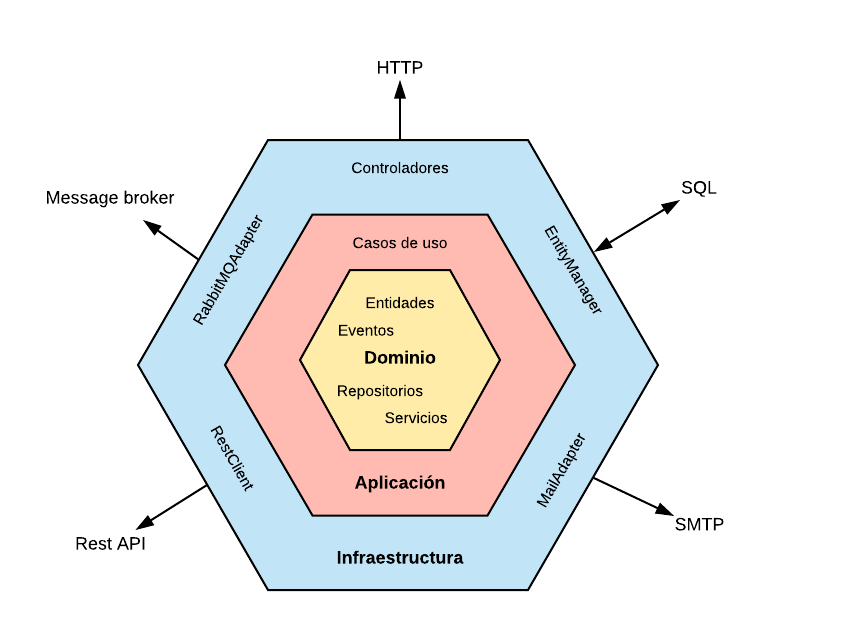
\includegraphics[width=0.8\textwidth]{Fotos/ArquitecturaHexagonal.png}
    \caption{Esquema conceptual de la orientación hexagonal del proyecto; no representa literalmente toda la jerarquía de paquetes.}
    \label{fig:arquitectura-hexagonal}
\end{figure}

\subsection{Estructura y componentes del sistema}

\subsubsection{Módulos del backend Java}

La base compartida de todo el sistema reside en el paquete \textit{shared}. La clase abstracta \textit{BaseEntity} dota a todas las entidades de la base de datos de tres campos estandarizados: un identificador autogenerado, una marca de tiempo de creación y un indicador de borrado lógico. El uso de borrado lógico en lugar de eliminación física garantiza la trazabilidad histórica de todas las operaciones: cualquier baja se expresa como una actualización de estado sin destruir el registro original \parencite{fowler_patterns_2002}. En un sistema contable, responder a qué capital tenía una estrategia al detenerse o por qué fue cerrada una posición es un requisito del dominio, no una conveniencia de implementación.

El módulo de \textbf{trading en tiempo real} es el núcleo operativo del sistema. La entidad \textit{InstanciaEstrategia} modela una configuración activa de ejecución: almacena el nombre de la estrategia, el capital asignado con precisión decimal, los parámetros de riesgo y el estado de ciclo de vida, que puede ser activa, detenida o terminada. \textit{Posicion} representa una operación de mercado individual, registrando el símbolo negociado, el precio de entrada exacto y un indicador de posición abierta que el motor consulta para evitar órdenes duplicadas sobre el mismo par. El historial financiero se construye con \textit{LedgerEntry}, un registro inmutable de cada movimiento de capital cuyo tipo se expresa mediante \textit{LedgerType}, que cubre ocho situaciones posibles: capital disponible, reservado, comprometido, margen comprometido, beneficio realizado, beneficio no realizado, comisión y estrategia pausada. La cartera digital implementa un doble saldo, formado por el balance real y el balance disponible, que impide sobregiros cuando varias estrategias compiten simultáneamente por el mismo capital. En la capa de aplicación, \textit{PaperTradingService} simula la ejecución de órdenes y valida las reglas de riesgo, mientras que \textit{AccountingService} actúa como único responsable de todas las operaciones monetarias, operando siempre con bloqueos de escritura para garantizar consistencia \parencite{goetz_java_concurrency_2006}. \textit{StrategyRuntimeCoordinator} gestiona el ciclo de vida de los procesos Python de trading mediante un grupo de hilos virtuales de la JDK 21 \parencite{goetz_jep444_2023}, lo que permite lanzar una instancia por estrategia activa sin saturar el grupo de hilos del sistema operativo y manteniendo un modelo de programación secuencial idiomático \parencite{goetz_java_concurrency_2006}.

La robustez financiera del sistema descansa en tres garantías transaccionales complementarias. Los repositorios de cartera digital e instancia de estrategia aplican bloqueos pesimistas de escritura exclusiva, impidiendo que dos hilos modifiquen el mismo saldo de forma simultánea y evitando así las inconsistencias contables que pueden surgir en escenarios de ejecución concurrente \parencite{goetz_java_concurrency_2006,oracle_mysql_acid_2024}. Todos los movimientos monetarios pasan obligatoriamente por \textit{AccountingService}, que los envuelve en transacciones atómicas con garantía de reversión completa ante cualquier fallo: si algún paso falla, el balance real, el balance disponible y el libro mayor vuelven al estado anterior sin dejar registros parciales \parencite{spring_data_jpa_2024,kleppmann_designing_2017}. El libro mayor actúa además como registro de auditoría permanente: dado que sus entradas son inmutables, es posible reconstruir el estado financiero de cualquier cartera en cualquier instante histórico, lo que facilita la verificación de discrepancias \parencite{lopez_de_prado_advances_2018,fowler_patterns_2002}.

El módulo de \textbf{backtesting} permite validar el comportamiento de una estrategia sobre datos reales sin riesgo financiero \parencite{pardo_evaluation_2008}. La entidad \textit{Vela} almacena los datos de precio y volumen con precisión decimal de ocho cifras y marca temporal en milisegundos. \textit{VelaDTO} emplea cadenas de texto para los precios al deserializar desde la interfaz de Binance, evitando pérdidas de precisión numérica durante la transferencia. \textit{BacktestingService} recupera las velas, serializa el mensaje en el formato binario del protocolo y lo envía al motor Python; a continuación, recibe los resultados estadísticos (tasa de acierto, factor de ganancia, caída máxima y ratio de Sharpe) y los persiste en un archivo de valores separados por comas.

El módulo de \textbf{descarga de datos de mercado} cubre el flujo de extracción, transformación y carga de datos históricos. \textit{FetchService} implementa la sincronización incremental: consulta la última vela almacenada y solicita a Binance únicamente los datos nuevos, persistiéndolos en lotes mediante inserciones masivas nativas \parencite{oracle_mysql_insert_opt_2024}, pues la sobrecarga de seguimiento de contexto del mapeador objeto-relacional resulta inasumible a ese volumen en tiempo interactivo; la sentencia condicional de actualización garantiza además la idempotencia de las descargas repetidas y repara automáticamente huecos que pudieran haber quedado por desconexiones o cambios de interfaz, resincronizando desde el punto de ruptura sin necesidad de intervención manual \parencite{kimball_data_2004,pardo_evaluation_2008}. El motor Python gestiona el acceso a la interfaz de Binance respetando sus límites de tasa mediante dos estrategias complementarias: de forma proactiva, introduce pausas entre peticiones según los umbrales conocidos de la interfaz; de forma reactiva, interpreta los códigos de respuesta 429 y 418 aplicando retroceso exponencial con reintentos automáticos \parencite{binance_rate_limits_2024,kleppmann_designing_2017}. \textit{MarketDataService} orquesta en una sola llamada la descarga y el cálculo de indicadores. \textit{IndicatorsService} delega el cálculo al motor Python y persiste los resultados como entidades de indicador técnico.

El módulo de \textbf{inteligencia artificial y optimización} gestiona el entrenamiento supervisado y la búsqueda de la configuración óptima de los modelos. \textit{AITrainingService} prepara el conjunto de datos, selecciona el tipo de modelo y lo envía al motor Python, recibiendo a cambio las métricas de evaluación. \textit{AIOptimizationService} extiende ese flujo incorporando parámetros de búsqueda como el número de ensayos y el umbral mínimo de exactitud aceptable, delegando al motor la búsqueda bayesiana mediante Optuna \parencite{feurer_hyperparameter_2019}.

El módulo de \textbf{gestión de usuarios y carteras digitales} implementa el acceso a la plataforma con las garantías de seguridad propias del software financiero \parencite{owasp_password_2024}. \textit{Usuario} es una clase Java sin dependencias de infraestructura: su persistencia se delega a un adaptador que traduce entre la representación de dominio y la entidad de base de datos mediante un mapeador dedicado. \textit{UsuarioApplicationService} implementa los casos de uso de creación y autenticación de usuarios, aplicando cifrado de contraseña con BCrypt \parencite{provos_bcrypt_1999}: un algoritmo adaptativo que incorpora una sal aleatoria por usuario, de modo que las contraseñas nunca se almacenan en texto plano y la dificultad de cómputo puede endurecerse sin modificar el esquema de datos. Las credenciales de acceso a la base de datos se inyectan en tiempo de arranque mediante variables de entorno cargadas desde un archivo local excluido del control de versiones; si alguna variable obligatoria está ausente, la aplicación falla de forma inmediata y visible en lugar de propagarse como un error silencioso en ejecución \parencite{kleppmann_designing_2017}. \textit{WalletService} gestiona la creación y consulta de carteras en modo de operativa simulada. \textit{SessionManager} mantiene en memoria el usuario autenticado activo, restringe el acceso a cualquier operación sensible a sesiones previamente autenticadas y registra un gancho de cierre que detiene todas las estrategias activas al apagar la aplicación \parencite{gamma_design_1994}.

Entre las utilidades transversales, \textit{PathConfig} centraliza la resolución de rutas del sistema de archivos con independencia del directorio desde el que se ejecute la aplicación; \textit{AppConstants} define las constantes del contrato entre Java y Python, como claves de objetos serializados y cabeceras de archivos; y \textit{IpcMessagePackCodec} implementa el protocolo binario de bajo nivel, encapsulado en un registro inmutable con versión de protocolo, tipo de mensaje, identificador de correlación y contenido.

\subsubsection{Patrones de diseño aplicados}
\label{sec:patrones}

La arquitectura hace uso explícito de varios patrones de diseño reconocibles en puntos concretos del código \parencite{gamma_design_1994,fowler_patterns_2002}. El patrón \textbf{Repositorio} aparece en todas las interfaces de acceso a datos, como \textit{LedgerRepository} o \textit{WalletRepository}, abstrayendo los detalles de consulta y persistencia frente a los servicios de aplicación. El patrón \textbf{Comando} está presente tanto en el gestor principal de la interfaz de línea de comandos como en cada clase de comando individual, que encapsula la lógica de una acción y delega su ejecución al servicio de aplicación correspondiente. El patrón \textbf{Fachada} se aplica en \textit{PythonBridgeFacade}, que simplifica la interacción con los procesos Python detrás de una interfaz uniforme, ocultando los detalles del protocolo binario a los servicios que lo usan. El patrón \textbf{Constructor} se utiliza en \textit{PythonBridgeRequest} para configurar cada invocación al motor Python de forma legible y sin constructores de múltiples parámetros. El patrón \textbf{Registro único} aparece en \textit{SessionManager} gestionado por Spring, garantizando que solo exista una sesión activa en todo momento. Por último, en el motor Python, la jerarquía basada en \textit{BaseStrategy} introduce el patrón \textbf{Estrategia}: cada implementación concreta define los mismos tres métodos obligatorios sin modificar el motor de ejecución \parencite{gamma_design_1994}.

\subsubsection{Motor Python}

Java actúa como orquestador del sistema por su tipado estático, soporte transaccional ACID y modelo de concurrencia basado en hilos virtuales \parencite{goetz_java_concurrency_2006}; Python se incorpora como motor de cálculo por disponer del ecosistema de análisis de datos y aprendizaje automático más maduro del mercado \parencite{hilpisch_python_2018,goodfellow_deep_2016}. El subsistema Python tiene una estructura intencionalmente sencilla. Se organiza en una única carpeta de scripts, donde cada archivo corresponde a un motor que se ejecuta como un proceso independiente invocado por el orquestador Java. Los motores disponibles cubren las siguientes funciones: descarga de velas de Binance, cálculo de indicadores técnicos, simulación histórica de estrategias, trading en tiempo real con reglas clásicas, trading en tiempo real con modelo neuronal, entrenamiento supervisado y optimización de configuraciones. Todos comparten un módulo de utilidades comunes y el módulo del protocolo de comunicación. La carpeta de estrategias, separada de los motores, contiene la clase base abstracta \textit{BaseStrategy} y las implementaciones concretas. Esta separación garantiza que añadir una nueva estrategia no requiera modificar ningún motor existente. La descarga de datos históricos aprovecha además la concurrencia de Python mediante un grupo de hilos que lanza múltiples peticiones simultáneas a la interfaz de Binance, reduciendo significativamente el tiempo total de descarga cuando se solicitan varios periodos o símbolos a la vez \parencite{python_concurrent_futures_2024,binance_rest_api_2024}.

\subsection{Comunicación entre procesos}
\label{sec:ipc}

La comunicación entre el orquestador Java y los motores Python es un componente crítico de la arquitectura. Se ha definido un protocolo versionado de forma explícita para garantizar compatibilidad y permitir su evolución sin romper el funcionamiento existente \parencite{richards_software_2022}.

Todo mensaje intercambiado respeta una estructura envolvente con cuatro campos: la versión del protocolo, el tipo de mensaje como código semántico de la operación (solicitud de descarga, respuesta de indicadores, error, señal en tiempo real, entre otros), un identificador de correlación único por petición para asociar solicitudes y respuestas \parencite{hohpe_enterprise_2003}, y el contenido específico de la operación en formato binario. Para evitar problemas de sincronización en las tuberías de comunicación, cada mensaje va precedido de un entero de cuatro bytes en orden de red que especifica la longitud exacta del cuerpo. El contenido se serializa en \textbf{MessagePack} \parencite{furuhashi_msgpack_2013}, un formato binario más compacto que su equivalente en texto plano y sin pérdida de compatibilidad de tipos \parencite{kleppmann_designing_2017}. El volumen de datos intercambiados por sesión puede alcanzar cientos de miles de velas con sus indicadores calculados, lo que convierte la eficiencia de serialización en un requisito práctico; el prefijo de longitud de cuatro bytes simplifica además la lectura del flujo sin necesidad de delimitadores en el contenido.

La comunicación utiliza la salida estándar como canal exclusivo para el flujo de mensajes binarios, mientras que los registros y errores se envían por el canal de error estándar, garantizando que el orquestador lea el flujo de datos sin interferencias \parencite{newman_building_2015}. Para el trading en tiempo real, el motor Python emite líneas de control con un prefijo de señal seguidas del contenido de la orden en formato estructurado. El coordinador Java lee cada línea y delega en el analizador de protocolo para identificar las señales; una vez reconocidas, las entrega al servicio de operativa simulada para su procesamiento contable.

La convención de códigos de salida permite al orquestador tomar decisiones de recuperación de forma automatizada \parencite{richards_software_2022}: el código cero indica ejecución exitosa; el uno señala un error de lógica no recuperable sin intervención del usuario, como una estrategia inválida o un modelo no entrenado; el dos corresponde a un error en los datos de entrada; y el tres indica una interrupción por tiempo de espera agotado o cierre externo del proceso.

Para evitar que procesos bloqueados consuman recursos indefinidamente, se definen tiempos de espera diferenciados según la operación \parencite{kleppmann_designing_2017}: 120 segundos para el arranque del proceso, que incluye la importación de bibliotecas pesadas como TensorFlow; 300 segundos de inactividad máxima para operaciones de descarga o cálculo de indicadores; 900 segundos para la simulación histórica, aunque el caso típico concluye en menos de un minuto \parencite{pardo_evaluation_2008}; 1800 segundos para el entrenamiento de modelos, que puede incluir validación cruzada sobre series temporales \parencite{lopez_de_prado_advances_2018}; y 3600 segundos para la optimización de hiperparámetros, cuya duración puede prolongarse en función del espacio de búsqueda definido. Si un proceso supera alguno de estos umbrales sin producir actividad, el orquestador lo termina forzosamente y lo registra con el código de salida tres.

\subsection{Ventajas y desventajas de la arquitectura}

La adopción de este esquema responde a una evaluación de sus beneficios frente a las necesidades del sistema \parencite{treleaven_algorithmic_2013}.

Entre las ventajas, la más relevante es la \textbf{mantenibilidad}. Si fuera necesario cambiar el motor de base de datos de MySQL a otro sistema, solo se vería afectado el adaptador de persistencia; la lógica de las estrategias en Python y los servicios Java permanecerían intactos \parencite{spring_data_jpa_2024,martin_clean_architecture_2017}. Una consecuencia directa de esa separación es la \textbf{facilidad para escribir pruebas}: los servicios de aplicación dependen de interfaces y no de implementaciones concretas, lo que permite verificar la lógica de contabilidad sin necesidad de lanzar los procesos de inteligencia artificial ni conectarse a la base de datos real \parencite{martin_clean_architecture_2017,evans_domain_driven_2003}. Finalmente, la \textbf{independencia entre subsistemas} permite trabajar de forma aislada en la robustez del orquestador Java mientras se perfeccionan los modelos matemáticos en Python, siempre que el contrato de datos entre ambas partes se mantenga constante \parencite{hilpisch_python_2018,newman_building_2015}.

Entre las limitaciones, la principal es el \textbf{volumen de código adicional}. El flujo de datos requiere transformar entidades en objetos de transferencia al pasar de una capa a otra, lo que incrementa el código necesario frente a una arquitectura más directa \parencite{richards_software_2022,martin_clean_architecture_2017}. Esta limitación se mitiga mediante el uso de Lombok para la generación automática de constructores y mapeadores dedicados \parencite{lombok_project_2024}. La otra limitación es la \textbf{latencia acumulada}: en sistemas de trading de altísima frecuencia, el paso de información a través de múltiples capas puede introducir pequeños retardos \parencite{treleaven_algorithmic_2013}. Para los intervalos de tiempo gestionados en este proyecto, velas de un minuto o superiores, este impacto es despreciable frente a la seguridad transaccional obtenida \parencite{oracle_mysql_acid_2024,pardo_evaluation_2008}.
\section{Indicadores Técnicos Implementados}
\label{sec:indicadores}

Los indicadores técnicos son herramientas matemáticas que transforman la acción del precio en señales interpretables, con el objetivo de identificar tendencias, medir impulso y detectar condiciones extremas del mercado. Murphy los clasifica en dos grandes familias \parencite{murphy_technical_1999}: los \textit{seguidores de tendencia} (\textit{trend-following}), como las medias móviles, que funcionan mejor en mercados con dirección definida; y los \textit{osciladores}, como el RSI y el MACD, que resultan más útiles en mercados laterales o para confirmar el agotamiento de una tendencia. El proyecto implementa los representantes más canónicos de ambas familias.

La razón fundamental para incorporar indicadores técnicos en un sistema de trading algorítmico es que permiten convertir una observación subjetiva del mercado en una regla matemática objetiva y reproducible. Un analista humano podría intuir que el precio ``lleva demasiado tiempo subiendo'', pero un algoritmo necesita una condición numérica precisa para actuar: RSI $> 70$, cruce del MACD, o precio por debajo de su SMA. Los indicadores son, en este sentido, el lenguaje común entre el análisis financiero y el código \parencite{chan_algorithmic_2013}.

\subsection{La Estrategia Base del Sistema}

El proyecto estructura las estrategias de trading mediante una jerarquía de clases Python basada en una clase abstracta (\textit{Abstract Base Class}) que define el contrato formal que toda estrategia debe satisfacer. La clase declara cinco métodos abstractos obligatorios: una función que recibe el conjunto de datos de velas y lo devuelve enriquecido con los indicadores calculados; dos funciones que evalúan las condiciones de apertura y cierre de posición en una vela concreta; y dos funciones que determinan los niveles de gestión del riesgo. Esta abstracción permite que los motores de \textit{backtesting}, tiempo real, entrenamiento y optimización operen de forma genérica con cualquier estrategia registrada sin conocer sus detalles internos.

La implementación concreta de referencia tiene como propósito verificar que el pipeline completo del sistema funcione de extremo a extremo con una estrategia funcional y representativa. Define un período de calentamiento de 20 velas y calcula ocho indicadores mediante la función de cálculo de indicadores, agrupados en dos familias según su función:

\begin{description}
    \item[Señales de trading (reglas clásicas)] Evaluadas directamente por las funciones de apertura y cierre de posición: la brecha relativa entre EMA rápida y lenta, el RSI de período 6, el retorno del último \textit{tick} y el \textit{z-score} del volumen.
    \item[Contexto de mercado para ML] Usados exclusivamente como \textit{features} en el módulo de entrenamiento y optimización: el retorno de tres velas, el ATR normalizado, el \textit{Percent B} de Bollinger y la tasa de cambio de 5 períodos.
\end{description}

Los indicadores de ambas familias se describen en las subsecciones siguientes.

\subsection{Indicador: Media Móvil Simple (SMA)}

La Media Móvil Simple es, según Murphy, el indicador técnico más ampliamente utilizado y el punto de partida para cualquier análisis de tendencia \parencite{murphy_technical_1999}. Su funcionamiento se basa en suavizar la acción del precio calculando el promedio aritmético de los últimos $n$ precios de cierre, eliminando el ruido de las fluctuaciones diarias y revelando la dirección subyacente del mercado:

$$\text{SMA}_n(t) = \frac{1}{n} \sum_{i=0}^{n-1} \text{close}(t-i)$$

\textbf{Por qué es una buena idea usarla.} La SMA cumple una función esencial en cualquier sistema algorítmico: actúa como filtro de tendencia. Operar en la dirección de la tendencia es uno de los principios más consolidados del trading; la SMA permite cuantificarlo de forma objetiva. Cuando el precio se mantiene por encima de su media, el sistema restringe las operaciones bajistas y favorece las alcistas, evitando que el algoritmo opere ``contra la corriente''. Además, su cálculo es computacionalmente trivial, lo que la hace ideal para su uso en tiempo real sobre grandes volúmenes de velas sin impacto en la latencia.

La interpretación operativa es directa: cuando el precio cotiza por encima de su media móvil, la tendencia es alcista; cuando cotiza por debajo, es bajista. Murphy enfatiza especialmente el valor de los cruces entre dos medias de distinto período como señales de entrada y salida: el cruce de la media de 50 períodos por encima de la de 200 (\textit{Golden Cross}) marca el inicio potencial de una tendencia alcista sostenida, mientras que el cruce inverso (\textit{Death Cross}) anticipa una tendencia bajista \parencite{murphy_technical_1999}.

La limitación inherente de la SMA es su \textit{time lag}: al asignar igual peso a todas las observaciones de la ventana, reacciona con cierto retraso ante los giros del mercado. A mayor período $n$, mayor suavizado pero también mayor retardo en la señal.

\subsection{Indicador: Media Móvil Exponencial (EMA)}

La Media Móvil Exponencial surge como respuesta directa a la limitación de retardo de la SMA. A diferencia de ésta, la EMA asigna un peso exponencialmente decreciente a las observaciones pasadas, otorgando mayor relevancia a los precios más recientes y reaccionando con mayor agilidad ante los cambios de tendencia \parencite{murphy_technical_1999}:

$$\text{EMA}_n(t) = \alpha \cdot \text{close}(t) + (1-\alpha) \cdot \text{EMA}_n(t-1)$$

donde el factor de suavizado $\alpha = \frac{2}{n+1}$ controla la velocidad de adaptación: valores altos de $\alpha$ (períodos cortos) producen una EMA más reactiva pero más ruidosa, mientras que valores bajos (períodos largos) generan una curva más suave pero más lenta. La EMA aborda este problema priorizando matemáticamente los datos recientes, lo que la hace especialmente valiosa en mercados de alta volatilidad como las criptomonedas \parencite{katsiampa_volatility_2017}.

\textbf{Por qué es una buena idea usarla.} En un sistema de trading en tiempo real, la velocidad de reacción ante un cambio de tendencia tiene un impacto directo en la rentabilidad: entrar tarde en una tendencia implica asumir más riesgo y capturar menos beneficio. La EMA aborda este problema priorizando matemáticamente los datos recientes, lo que la hace especialmente valiosa en mercados de alta volatilidad como las criptomonedas, donde los movimientos bruscos son frecuentes y una media lenta puede generar señales obsoletas. En el contexto del proyecto, la EMA es además el bloque constructivo del MACD, por lo que su correcta implementación es un requisito previo para el indicador de impulso más utilizado del sistema.

En la estrategia de referencia del sistema, la EMA se implementa con dos períodos deliberadamente cortos: EMA rápida (período 3) y EMA lenta (período 8). Su diferencia relativa, denominada brecha entre medias exponenciales, se define como:
$$\text{ema\_gap}(t) = \frac{\text{EMA}_3(t) - \text{EMA}_8(t)}{\text{close}(t)}$$
Un valor positivo de esta métrica indica impulso alcista a corto plazo.
La condición de que dicha brecha supere $0{,}001$ exige que este impulso supere el 0.1\%
del precio, filtrando cruces espurios de escaso recorrido.

\subsection{Indicador: Relative Strength Index (RSI)}

El RSI fue desarrollado por J. Welles Wilder y presentado en su obra \textit{New Concepts in Technical Trading Systems} (1978). Murphy lo incorpora como el oscilador de referencia para medir la \textit{velocidad y magnitud} de los movimientos de precio, evaluando si un activo se encuentra en zona de sobrecompra o sobreventa \parencite{murphy_technical_1999}. A diferencia de las medias móviles, el RSI no sigue la tendencia sino que la cuestiona cuando alcanza niveles extremos.

Su cálculo se basa en la relación entre las ganancias medias y las pérdidas medias durante una ventana de $n$ períodos:

$$\text{RSI} = 100 - \frac{100}{1 + \text{RS}}, \quad \text{donde} \quad \text{RS} = \frac{\overline{\text{ganancias}_n}}{\overline{\text{pérdidas}_n}}$$

El oscilador se mueve en el rango $[0, 100]$ y su interpretación operativa sigue los umbrales canónicos establecidos por Wilder y refrendados por Murphy: una lectura por encima de 70 indica que el activo está \textbf{sobrecomprado} (\textit{overbought}), sugiriendo que la presión compradora puede estar agotándose y que podría producirse una corrección a la baja; una lectura por debajo de 30 señala \textbf{sobreventa} (\textit{oversold}), indicando que la presión vendedora puede estar llegando a su límite y que podría producirse un rebote.

\textbf{Por qué es una buena idea usarlo.} El RSI resuelve un problema fundamental del trading algorítmico: evitar comprar en máximos y vender en mínimos. Las medias móviles por sí solas son ciegas ante el agotamiento de una tendencia; pueden señalar ``tendencia alcista'' incluso cuando el precio lleva semanas subiendo de forma casi vertical y una corrección es estadísticamente probable. El RSI introduce una dimensión temporal de fatiga del mercado que las medias no capturan. En la estrategia de referencia del sistema, el RSI se calcula con un período de 6 velas en lugar del estándar de 14 propuesto por Wilder, priorizando la reactividad ante cambios rápidos de impulso típicos de \textit{timeframes} cortos en criptomonedas. Este RSI de corto plazo actúa como condición de filtro: solo se permite abrir una posición de compra si no ha superado el umbral de 55 (zona neutral-alta), reduciendo la probabilidad de entrar en un movimiento alcista ya avanzado. Adicionalmente, Murphy destaca el fenómeno de la \textbf{divergencia} como una de las señales más fiables del indicador: cuando el precio marca un nuevo máximo pero el RSI no logra superarlo, se produce una divergencia bajista que advierte de una posible pérdida de impulso y reversión de tendencia, incluso antes de que el precio lo confirme \parencite{murphy_technical_1999}.

\subsection{Indicador: Moving Average Convergence Divergence (MACD)}

El MACD, desarrollado por Gerald Appel, es el oscilador de impulso por excelencia y ocupa un lugar central en el análisis técnico moderno tal y como lo describe Murphy \parencite{murphy_technical_1999}. Combina las propiedades de seguimiento de tendencia de las medias móviles con la sensibilidad de un oscilador, ofreciendo así información tanto sobre la dirección como sobre la fuerza del movimiento.

El indicador se construye en tres componentes:

\begin{itemize}
    \item \textbf{Línea MACD:} diferencia entre la EMA de 12 y la EMA de 26 períodos. Mide la convergencia o divergencia entre ambas medias; cuando es positiva, la EMA rápida está por encima de la lenta (impulso alcista), y cuando es negativa, ocurre lo contrario.
    \item \textbf{Línea de señal:} EMA de 9 períodos aplicada sobre la propia línea MACD. Actúa como suavizador y genera las señales operativas.
    \item \textbf{Histograma MACD:} diferencia entre la línea MACD y la señal. Su utilidad principal es anticipar los cruces antes de que se produzcan: cuando las barras del histograma se reducen, un cruce de señal es inminente.
\end{itemize}

$$\text{MACD}(t) = \text{EMA}_{12}(t) - \text{EMA}_{26}(t)$$
$$\text{Signal}(t) = \text{EMA}_9\bigl(\text{MACD}\bigr)(t)$$
$$\text{Histograma}(t) = \text{MACD}(t) - \text{Signal}(t)$$

\subsection{Indicador: \textit{Z-score} de Volumen}

El volumen de negociación es el indicador más directo de la participación del mercado en un movimiento de precio: un movimiento acompañado de volumen alto refleja mayor consenso entre participantes y es estadísticamente más significativo que el mismo movimiento con volumen escaso \parencite{murphy_technical_1999}.

El sistema normaliza el volumen mediante el \textit{z-score} respecto a su distribución en las últimas 20 velas: $$\text{vol\_z}(t) = \frac{V(t) - \overline{V}_{20}(t)}{\sigma_{V_{20}}(t)}$$ Un valor del \textit{z-score} de volumen superior a cero indica que el volumen supera su media histórica reciente. En la estrategia de referencia, la condición de apertura exige que este \textit{z-score} supere $0{,}5$, requiriendo que el volumen supere la media en al menos medio punto de desviación típica para confirmar la señal.

\subsection{Indicador: ATR Normalizado}

El \textit{Average True Range} (ATR), propuesto por Wilder, es el indicador de volatilidad realizada de referencia en el análisis técnico \parencite{murphy_technical_1999}. Mide el rango de movimiento real de cada vela, considerando posibles huecos (\textit{gaps}) entre sesiones: $$\text{TR}(t) = \max\bigl(\text{high}_t - \text{low}_t,\;|\text{high}_t - \text{close}_{t-1}|,\; |\text{low}_t - \text{close}_{t-1}|\bigr)$$ $$\text{ATR}_n(t) = \frac{1}{n}\sum_{i=0}^{n-1}\text{TR}(t-i)$$ En la estrategia de referencia, el ATR de 14 períodos se normaliza dividiendo entre el precio de cierre, obteniendo una medida de volatilidad relativa comparable entre activos y niveles de precio. Este indicador no interviene en las reglas clásicas de apertura, sino que aporta contexto de volatilidad como \textit{feature} para el módulo de ML.

\subsection{Indicador: Bandas de Bollinger}

Las Bandas de Bollinger posicionan el precio actual dentro de su distribución estadística reciente, definiendo bandas superior e inferior a $k$ desviaciones típicas de la media móvil de $n$ períodos \parencite{murphy_technical_1999}: $$\text{Banda}_{\pm}(t) = \text{SMA}_n(t) \pm k\,\sigma_n(t)$$ El \textit{Percent B} cuantifica la posición relativa del precio dentro de las bandas, normalizado en el intervalo $[0, 1]$: $$\text{bb\_pct}(t) = \frac{\text{close}(t) - \text{Banda}_{-}(t)}{\text{Banda}_{+}(t) - \text{Banda}_{-}(t)}$$ Un valor cercano a 0 indica que el precio se aproxima a la banda inferior (posible sobreventa), mientras que un valor cercano a 1 sugiere proximidad a la banda superior (posible sobrecompra). En la estrategia de referencia se emplean los parámetros estándar ($n=20$, $k=2$). El indicador se usa exclusivamente como \textit{feature} de ML.

\subsection{Indicador: Tasa de Cambio (ROC)}

La Tasa de Cambio cuantifica el porcentaje de variación del precio respecto a $n$ períodos anteriores, midiendo directamente la velocidad del movimiento \parencite{murphy_technical_1999}: $$\text{ROC}_n(t) = \frac{\text{close}(t) - \text{close}(t-n)}{\text{close}(t-n)} \times 100$$ En la estrategia de referencia se calcula la tasa de cambio de 5 períodos, que captura el impulso acumulado en los últimos cinco \textit{ticks}. A diferencia del retorno de un solo período, el ROC proporciona una visión del movimiento sostenido en un horizonte más amplio, lo que resulta especialmente útil para que el modelo de ML distinga entre impulsos sostenidos y fluctuaciones puntuales.

\subsection{Relación entre Indicadores y Uso Combinado}

Murphy insiste en que ningún indicador debe emplearse de forma aislada \parencite{murphy_technical_1999}. La práctica profesional consiste en combinar indicadores de distintas familias para obtener confirmación cruzada: una señal de compra del MACD gana fiabilidad cuando el RSI se encuentra por debajo de 50 (sin llegar a sobreventa) y el precio ha superado su SMA, ya que los tres instrumentos coinciden en señalar impulso alcista desde diferentes perspectivas matemáticas. Esta filosofía de confirmación múltiple es precisamente la base sobre la que se diseñan las estrategias implementadas en este proyecto \parencite{murphy_technical_1999}.

Cada indicador es, individualmente, propenso a generar falsas señales en determinadas condiciones de mercado: la SMA las genera en mercados laterales, el RSI puede permanecer en zona de sobrecompra durante tendencias alcistas prolongadas, y el MACD puede producir cruces frecuentes en períodos de baja volatilidad. La combinación de indicadores actúa como un sistema de votación: solo se ejecuta una orden cuando varios instrumentos independientes coinciden, reduciendo drásticamente la tasa de falsas señales a costa de perder algunas oportunidades. En la estrategia de referencia, la apertura de una posición de compra requiere que cuatro condiciones independientes se cumplan simultáneamente: una brecha entre medias exponenciales superior a $0{,}001$ (tendencia alcista de corto plazo), un RSI de corto plazo inferior a $55$ (impulso no agotado), un retorno positivo en el último \textit{tick} y un \textit{z-score} de volumen superior a $0{,}5$ (volumen por encima de su media histórica reciente). Las condiciones de venta son simétricas. Esta exigencia de confirmación múltiple es la razón por la que la función de cálculo de indicadores de la clase base está diseñada para acoger múltiples indicadores simultáneamente \parencite{murphy_technical_1999}.

\subsection{Período de Calentamiento}

Todos los indicadores descritos requieren un número mínimo de velas históricas antes de poder generar valores válidos. Este período inicial, conocido como \textit{warmup period}, produce valores indefinidos que deben descartarse antes de cualquier análisis o entrenamiento de modelos, ya que su inclusión introduciría ruido en el pipeline de ML y podría sesgar las métricas de evaluación.

El período de calentamiento del sistema se fija en el máximo entre todos los indicadores activos. En la estrategia de referencia, dicho período está fijado en 20 velas, valor que cubre la ventana de estabilización de las medias de volumen y de las Bandas de Bollinger (ambas con ventana de 20 períodos). La clase base dispone de una función que calcula automáticamente el período máximo a partir de las constantes de período definidas en cada estrategia. Las filas de calentamiento se descartan antes de cualquier análisis o entrenamiento:

Esto garantiza que todos los indicadores son matemáticamente válidos en el DataFrame que alimenta los motores de backtesting y entrenamiento de modelos \parencite{mckinney_python_2022}.
\section{Módulo de Inteligencia Artificial y Validación Experimental}
\label{sec:ml}

La capacidad predictiva del sistema descansa en un módulo de aprendizaje
automático supervisado implementado en Python que integra ingeniería de
características dinámica, generación de etiquetas orientada al movimiento
real del mercado, validación temporal rigurosa y soporte para múltiples
familias de modelos \parencite{goodfellow_deep_2016}. El módulo delega en
cada estrategia la definición de sus propias características, lo que garantiza
que el motor de entrenamiento puede reutilizarse sin modificación mientras las
estrategias evolucionan.

\subsection{Ingeniería de características y generación de etiquetas}

Para construir el conjunto de datos de entrenamiento, el motor invoca el
método abstracto \textit{populate\_indicators()} de la estrategia activa,
que enriquece el marco de datos con los indicadores técnicos propios de esa
estrategia: si la estrategia emplea el índice de fuerza relativa y una media
móvil simple de veinte períodos, el método calcula y añade esas dos columnas;
si otra estrategia solo requiere el índice de fuerza relativa, el marco de
datos resultante tendrá únicamente esa característica adicional. A
continuación, \textit{get\_feature\_columns()} extrae todas las columnas no
pertenecientes al conjunto base precio-volumen (apertura, máximo, mínimo,
cierre, volumen), construyendo así la matriz de características $X$ de forma
dinámica y sin duplicación de código entre estrategias
\parencite{mckinney_python_2022}.

La generación de etiquetas sigue un enfoque prospectivo implementado en el
método \textit{get\_label()}: para cada vela en el instante $t$, la etiqueta
se determina comparando el precio de cierre de la vela siguiente $t+1$ con
el precio de cierre actual. Si el retorno supera un umbral configurable, la
etiqueta es $+1$ (expectativa de subida); si cae por debajo del umbral
negativo, la etiqueta es $-1$ (expectativa de bajada); en caso contrario, la
etiqueta es $0$ (mercado lateral). El umbral por defecto del 0,2\,\%
equilibra la sensibilidad de la señal con la frecuencia de etiquetas activas
\parencite{lopez_de_prado_advances_2018}. Este enfoque es deliberado: si las
etiquetas se derivasen directamente de las condiciones de compra o venta de la
estrategia, el modelo aprendería a memorizar la lógica booleana y no a
predecir el mercado, produciendo métricas artificialmente altas sin
rentabilidad real \parencite{goodfellow_deep_2016}.

El desequilibrio de clases es una consecuencia esperada en datos de
negociación algorítmica, donde la mayoría de los períodos no activan señales
comerciales \parencite{lopez_de_prado_advances_2018}. Este desequilibrio se
aborda en dos dimensiones. Desde el punto de vista de la evaluación, las
métricas se calculan con ponderación por la frecuencia real de cada clase,
evitando que las clases minoritarias sean invisibles en las estadísticas de
rendimiento \parencite{pedregosa_scikit_2011}. Desde el punto de vista del
entrenamiento, todos los modelos ajustan automáticamente el peso de cada clase
mediante \textit{compute\_class\_weight("balanced")} de scikit-learn, de modo
que la clase más escasa contribuye con mayor peso al gradiente de optimización;
cuando el desequilibrio es muy pronunciado, pueden aplicarse adicionalmente
técnicas de remuestreo sintético como SMOTE \parencite{chawla_smote_2002}. En
la práctica, distribuciones muy sesgadas, como el 71\,\% de etiquetas neutras
observado en algunas combinaciones de estrategia y marco temporal, señalan una
incompatibilidad entre la estrategia y el período histórico elegido y deben
motivar una revisión de los umbrales de señal o una ampliación del conjunto de
datos.

\subsection{Preparación del conjunto de datos}

Los datos enriquecidos con indicadores se preparan en tres etapas antes del
entrenamiento. En primer lugar, el período de calentamiento necesario para la
estabilización numérica de los indicadores se determina mediante
\textit{get\_warmup\_period()}, que devuelve el máximo de todos los períodos
configurados en la estrategia; las filas iniciales que no alcanzan ese mínimo
se descartan para evitar valores incompletos que distorsionarían el aprendizaje
\parencite{murphy_technical_1999}. En segundo lugar, se realiza una limpieza
defensiva del conjunto de datos: los valores infinitos se reemplazan por
valores nulos y las filas que los contienen se eliminan, registrando cuántas
filas se descartaron \parencite{mckinney_python_2022}. En tercer lugar, el
conjunto resultante se divide de forma estrictamente cronológica en proporciones
80/20: el ochenta por ciento más antiguo forma el conjunto de entrenamiento y
el veinte por ciento más reciente se reserva como conjunto de evaluación final,
que no participa en ningún momento del proceso de entrenamiento ni de la
búsqueda de hiperparámetros para preservar la causalidad temporal
\parencite{goodfellow_deep_2016,lopez_de_prado_advances_2018}.

Cada modelo entrenado persiste junto con sus metadatos: nombre de la
estrategia, tipo de modelo, lista de características utilizadas, distribución
de etiquetas del conjunto de datos y métricas de clasificación obtenidas. Este
registro permite auditar bajo qué condiciones se obtuvo cada resultado y
detectar el sobreajuste al histórico descrito por
\textcite{lopez_de_prado_advances_2018}. El motor genera adicionalmente un
archivo de valores separados por comas con las métricas de todos los ensayos
de optimización, lo que habilita un análisis posterior de la convergencia del
proceso.

\subsection{Algoritmos soportados y optimización de hiperparámetros}

El módulo admite cuatro familias de modelos seleccionables desde el orquestador
Java sin modificar el código de evaluación. XGBoost \parencite{chen_xgboost_2016}
actúa como modelo de referencia gracias a su capacidad de regularización
explícita, especialmente útil para filtrar indicadores técnicos ruidosos.
LightGBM \parencite{ke_lightgbm_2017} ofrece tiempos de entrenamiento
sustancialmente menores en conjuntos de datos de gran volumen mediante su
estrategia de crecimiento por hojas en lugar de por niveles. Los bosques
aleatorios reducen la varianza del modelo a través del muestreo por remplazo y
aportan una estimación de importancia de características que orienta la
revisión de la ingeniería de características. Las redes neuronales con
TensorFlow\,/\,Keras \parencite{goodfellow_deep_2016} exploran dependencias
complejas en las series de precios mediante arquitecturas configurables de capas
densas con abandono regularizador y detención anticipada. La disponibilidad de
varios modelos facilita la comparación controlada del rendimiento entre familias
de algoritmos bajo condiciones idénticas de entrenamiento y evaluación
\parencite{feurer_hyperparameter_2019}.

Para la búsqueda automática de la configuración óptima, el sistema emplea
Optuna \parencite{feurer_hyperparameter_2019}, una librería de optimización
bayesiana que usa el estimador de Parzen estructurado en árbol para descarta
iterativamente las regiones del espacio de búsqueda con baja probabilidad de
mejora. Un podador por mediana (\textit{MedianPruner}, con cinco ensayos de
arranque y diez pasos de calentamiento) interrumpe de forma anticipada los
ensayos cuyo rendimiento intermedio queda por debajo de la mediana de los
ensayos anteriores, reduciendo el coste computacional total.

La evaluación de cada ensayo sigue un esquema de partición de series
temporales con cinco divisiones por defecto (\textit{TimeSeriesSplit} de
scikit-learn) \parencite{pedregosa_scikit_2011}: en cada partición, el modelo
se entrena sobre el subconjunto cronológicamente anterior y genera predicciones
sobre el subconjunto posterior, de modo que ningún dato futuro contamina la
evaluación. Sobre las predicciones de la partición más reciente ---la que
contiene los datos más próximos al conjunto de evaluación final--- se ejecuta
una simulación histórica para obtener métricas de rendimiento real: tasa de
acierto, factor de ganancia y ratio de Sharpe. La puntuación compuesta que
guía la búsqueda es:
\begin{equation}
    \label{eq:composite_score}
    score = 0{,}25 \cdot F1_{vc} + 0{,}40 \cdot TA + 0{,}25 \cdot FG_{norm} + 0{,}10 \cdot RS_{norm} - \max(0,\, brecha - 0{,}05) \cdot 2
\end{equation}
donde $F1_{vc}$ es el F1 ponderado medio en las particiones de validación,
$TA$ es la tasa de acierto expresada como fracción entre cero y uno,
$FG_{norm} = \min(FG, 5) / 5$ es el factor de ganancia normalizado al
intervalo $[0,1]$, $RS_{norm} = \max(0, \min(RS/2, 1))$ es el ratio de Sharpe
normalizado, y $brecha = acc_{train} - acc_{vc}$ mide el sobreajuste. La
penalización se activa cuando la brecha supera el cinco por ciento,
desincentivando configuraciones que memorizan el conjunto de entrenamiento sin
generalizar \parencite{goodfellow_deep_2016}. La ponderación otorga mayor
peso a la tasa de acierto real (0,40) que a la calidad de clasificación
estadística (0,25), reflejando que el objetivo final es la rentabilidad
operativa y no la optimización de una métrica de aprendizaje aislada
\parencite{lopez_de_prado_advances_2018}.

Una vez completados todos los ensayos, el sistema selecciona los
hiperparámetros del ensayo con mayor puntuación compuesta y entrena con ellos
el modelo definitivo sobre la totalidad del conjunto de entrenamiento,
evaluándolo sobre el conjunto de test reservado para obtener las métricas
finales de exactitud, precisión, exhaustividad y F1. Los espacios de búsqueda
concretos empleados para cada familia de modelos, determinados
experimentalmente durante el desarrollo del proyecto, se recogen en el
Anexo~\ref{anx:hiperparametros}.

\section{Diagramas de Flujo}
A continuación se describen en detalle los procesos principales del sistema,
trazando el recorrido de cada comando desde la entrada en la CLI hasta la
respuesta final al usuario. El sistema expone veinte comandos operativos que
se pueden agrupar en seis familias funcionales: gestión de usuarios, gestión
de capital, obtención de datos, gestión de estrategias, inteligencia artificial
y consultas informativas.

% =============================================================================
\subsection{Gestión de Usuarios y Acceso}
% =============================================================================

La Figura~\ref{fig:login} muestra el flujo de entrada principal del usuario
a través de la interfaz de línea de comandos (CLI), incluyendo autenticación,
registro y ayuda. El \textit{dispatcher} principal de la CLI intercepta la
línea introducida y la enruta al comando correspondiente mediante el registro
de comandos inicializado al arrancar la aplicación. Todos los comandos
operativos verifican en primer lugar que exista una sesión activa antes de
ejecutar cualquier lógica; los comandos de autenticación, en cambio,
comprueban lo contrario: que el usuario no haya iniciado ya sesión.

\textbf{Flujo de registro (\texttt{signup}).}
El comando solicita nombre de usuario y contraseña de forma interactiva.
El caso de uso de creación de usuario comprueba, dentro de una transacción de
solo lectura, que no exista otro usuario activo con ese nombre en la base de
datos. Si el nombre está libre, la contraseña se transforma con BCrypt antes
de que el objeto usuario sea persistido: la contraseña en claro nunca se
almacena ni se transmite a la capa de persistencia. Si el nombre ya existe,
el sistema lo notifica al usuario y el registro no se completa. Esta decisión
de validar unicidad por nombre de usuario (en lugar de por correo electrónico)
simplifica el flujo de registro y la experiencia en la CLI, donde no hay
formulario web que facilite la entrada de texto largo.

\textbf{Flujo de autenticación (\texttt{login}).}
El comando solicita nombre de usuario y contraseña. El caso de uso de
autenticación recupera el hash almacenado para ese nombre y lo coteja con la
contraseña proporcionada usando BCrypt de Spring Security Crypto. Si la
verificación es positiva, el gestor de sesión registra el usuario en la
variable de sesión de la aplicación, habilitando todos los comandos
operativos. Si las credenciales son incorrectas, el sistema notifica el fallo
sin especificar qué campo falló, evitando revelar si el nombre de usuario
existe en la base de datos. Al apagar la aplicación, el gestor de sesión
detecta el cierre del contexto de Spring y liquida todas las estrategias
activas antes de que el proceso termine, garantizando que ningún proceso
Python quede huérfano.

\begin{figure}[H]
    \centering
    
\includegraphics[width=0.9\linewidth]{Fotos/diagramas-flujo/inicio-registro-ayuda.png}
    \caption{Flujo de autenticación (login/signup) y ayuda}
    \label{fig:login}
\end{figure}

% =============================================================================
\subsection{Gestión de Capital (\textit{Wallets})}
% =============================================================================

La Figura~\ref{fig:wallets} muestra el proceso de creación y consulta de
billeteras virtuales. La plataforma soporta billeteras de tipo papel
(\textit{paper trading}) para operar con capital simulado, y el ciclo de vida
de cada billetera está estrechamente ligado al del libro mayor contable
(\textit{ledger}), que registra cronológicamente todos los movimientos de
capital.

\textbf{Listado de billeteras (\texttt{lw}).}
El comando verifica que haya sesión activa y delega en el servicio de gestión
de billeteras, que consulta todas las billeteras asociadas al identificador del
usuario en sesión, ordenadas por nombre. Para cada
billetera se muestra el saldo real (\textit{equity} acumulado incluido PnL
realizado), el saldo disponible para nuevas operaciones y un indicador
\texttt{[EN USO]} cuando la billetera tiene estrategias activas. Esta
distinción entre saldo real y saldo disponible es fundamental: el saldo
disponible se reduce en el momento en que se activa una estrategia y no se
recupera hasta que ésta se liquida definitivamente, aunque se pause en medio.

\textbf{Creación de billetera (\texttt{mkpwallet}).}
El comando solicita nombre y saldo inicial. El servicio de gestión de
billeteras comprueba que no exista ya una billetera con ese nombre para el
usuario actual. Si el nombre está disponible y el saldo es positivo, se crea
la billetera con saldo real y saldo disponible iguales al depósito inicial y
tipo \texttt{WalletType.PAPER}. La billetera queda en estado inactivo hasta
que se asigne a una estrategia. Cuando una estrategia se activa, el servicio
contable adquiere un bloqueo pesimista sobre la billetera y sobre la propia
instancia de estrategia antes de restar el capital del saldo disponible;
este mecanismo previene condiciones de carrera en escenarios de concurrencia
en los que varias estrategias pudieran activarse simultáneamente sobre la
misma billetera. En ese mismo instante se registra en el libro mayor una
entrada de tipo \texttt{RESERVED} con importe negativo, garantizando la
trazabilidad completa de cada movimiento de fondos desde el depósito inicial
hasta la liquidación final.

\begin{figure}[H]
    \centering
    
\includegraphics[width=0.7\linewidth]{Fotos/diagramas-flujo/creacion-listado-wallets.png}
    \caption{Proceso de creación y listado de \textit{wallets}}
    \label{fig:wallets}
\end{figure}

% =============================================================================
\subsection{Obtención de Datos (ETL)}
% =============================================================================

El comando de descarga implementa un mecanismo incremental que minimiza las
peticiones a la API de Binance y garantiza la consistencia del almacén
histórico. El servicio de descarga distingue tres modalidades de
operación según el estado de la base de datos para el par símbolo/temporalidad
solicitado.

En la modalidad por defecto, el servicio consulta la marca temporal más
reciente registrada en base de datos para el par e intervalo solicitados. Si
no existe ningún dato previo, lanza una descarga histórica completa desde el
origen disponible en la API; si ya hay datos, calcula el primer instante
ausente sumando el intervalo de temporalidad a la última marca temporal
conocida y descarga únicamente las velas nuevas. En ambos casos delega en el
motor Python de descarga a través del puente de comunicación: el servicio Java
envía la configuración vía MessagePack y el motor Python responde con los datos
serializados en el mismo protocolo.

El motor Python contacta el punto de acceso de velas de Binance solicitando
hasta 1\,500 registros por petición. Para historiales largos ejecuta hasta
cinco descargas en paralelo (\texttt{MAX\_PARALLEL\_WORKERS = 5}) y emite
las velas al consumidor Java en bloques de 2\,000 registros
(\texttt{EMIT\_CHUNK\_SIZE = 2000}) para evitar marcos IPC de tamaño
excesivo. El motor aplica un tratamiento diferenciado a los errores de la API:
ante un código 429 (\textit{rate limit}) espera el número de segundos que la
propia API indica en la respuesta; ante un 418, señal de bloqueo temporal de
la IP, aplica una espera más larga; ante errores 5xx del servidor reintenta
con \textit{backoff} exponencial hasta un máximo de 300 segundos
(\texttt{MAX\_BACKOFF\_SEC = 300}). Esta lógica de resiliencia permite
completar descargas masivas de meses de datos sin intervención manual aunque la
API imponga \textit{throttling} intermitente.

En el lado Java, las velas recibidas se insertan en MySQL mediante operaciones
por lotes con actualización condicional: si ya existe un registro con la misma
marca temporal para ese par e intervalo, únicamente se actualizan el precio de
cierre y el volumen, lo que hace la operación idempotente y permite
reejecutar descargas sin riesgo de duplicar datos. El tamaño de lote es de
50\,000 registros por operación (\texttt{BATCH\_INSERT\_SIZE = 50000}), lo
que permite ingerir decenas de miles de velas en pocos segundos sin saturar la
conexión de base de datos.

El modo de detección y relleno de huecos se activa con el argumento
\texttt{--detect-gaps}. El detector itera sobre todas las marcas temporales
almacenadas para el par e intervalo indicados y compara pares consecutivos. Si
la diferencia entre dos marcas supera el intervalo esperado más una tolerancia
de un segundo (\texttt{TOLERANCE\_MS = 1\,000}), se registra un hueco. La
tolerancia evita falsos positivos debidos a ligeras imprecisiones de reloj en
los servidores de Binance. Para cada hueco detectado, el componente realiza
una descarga directa vía HTTP sobre ese rango concreto sin pasar por el
proceso Python, solicitando exactamente las velas comprendidas en la ventana
faltante. Este modo resulta especialmente útil cuando la base de datos ha
acumulado datos de varias sesiones de descarga con interrupciones intermedias.

% =============================================================================
\subsection{Gestión de Estrategias}
% =============================================================================

La Figura~\ref{fig:listado} muestra el flujo de consulta y listado de
estrategias. El sistema diferencia entre consultas a base de datos (instancias
persistidas) y consultas al sistema de archivos (scripts Python disponibles).
Los comandos \texttt{ls}, \texttt{lsa}, \texttt{lsd} y \texttt{lst} muestran,
respectivamente, todas las instancias, solo las activas, solo las detenidas y
solo las terminadas. En cada caso se ejecuta una consulta filtrada por estado,
excluyendo siempre los registros dados de baja lógica mediante
\textit{soft delete}. La columna de capital muestra el capital reservado para
esa instancia, que puede diferir del capital comprometido en operaciones
abiertas en ese instante. El comando \texttt{le} no consulta la base de datos:
lee el directorio de estrategias del proyecto mediante inspección del sistema
de ficheros y devuelve los módulos Python que exponen una clase válida que
extiende \texttt{BaseStrategy}.

\begin{figure}[H]
    \centering
    
\includegraphics[width=0.9\linewidth]{Fotos/diagramas-flujo/listado-estrategias.png}
    \caption{Flujo de comandos de listado (ls, le, lsa)}
    \label{fig:listado}
\end{figure}

La Figura~\ref{fig:gestion} detalla las operaciones de control del ciclo de
vida de una estrategia: pausar (\textit{stop}), reanudar (\textit{start}) y
liquidar (\textit{term}).

\textbf{Flujo stop.}
El comando \texttt{stop <id>} cancela el hilo virtual asociado a la instancia
y envía la señal de interrupción al proceso Python. Acto seguido, dentro de
una transacción, el servicio adquiere un bloqueo pesimista sobre la instancia
de estrategia y actualiza el estado a \texttt{DETENIDA} solo si en ese momento
se encontraba en estado \texttt{ACTIVA}, evitando transiciones de estado
inconsistentes. Los fondos reservados para esa instancia permanecen congelados
en la billetera: el saldo disponible no se recupera al pausar, lo que impide
que el usuario los reasigne a otra estrategia mientras la instancia sigue
persistida. La variante \texttt{stop -all} itera sobre todos los
identificadores de estrategias activas y aplica el mismo flujo a cada uno.

\textbf{Flujo start.}
El comando \texttt{start <id>} solo es aplicable a instancias en estado
\texttt{DETENIDA}. El servicio de ciclo de vida recupera la instancia de la
base de datos y verifica el estado antes de continuar; si el estado no es
\texttt{DETENIDA}, registra un error y retorna sin modificar nada. Si el
estado es correcto, actualiza el estado a \texttt{ACTIVA} dentro de una
transacción y, \emph{fuera} de ella, lanza el motor Python en un nuevo hilo
virtual con los símbolos persistidos en la instancia. Este diseño, que separa
deliberadamente el cambio de estado transaccional del lanzamiento del proceso
Python, evita situaciones en las que el proceso quede arrancado mientras la
transacción de base de datos falla y hace \textit{rollback}.

\textbf{Flujo term.}
El comando \texttt{term <id>} inicia la liquidación definitiva de la
instancia. El servicio detiene el proceso Python de la misma forma que
\texttt{stop} y, acto seguido, el componente contable adquiere un bloqueo
pesimista sobre la instancia, comprueba si queda capital reservado sin
comprometer y, en ese caso, lo devuelve íntegramente al saldo disponible de
la billetera registrando una entrada de tipo \texttt{AVAILABLE} en el libro
mayor. El estado de la instancia pasa a \texttt{TERMINADA} y ya no puede
reanudarse. La variante \texttt{term -all} solicita confirmación explícita al
usuario antes de proceder con todas las instancias activas.

\begin{figure}[H]
    \centering
    
\includegraphics[width=0.9\linewidth]{Fotos/diagramas-flujo/gestion-estrategias.png}
    \caption{Ciclo de vida: start, stop y term}
    \label{fig:gestion}
\end{figure}

% =============================================================================
\subsection{Backtesting}
% =============================================================================

La Figura~\ref{fig:backtest} muestra el flujo de validación histórica,
disponible en modo clásico (solo estrategia de reglas) y en modo con modelo
IA (estrategia más modelo supervisado).

El proceso comienza en la CLI: el comando \texttt{backtest} solicita de forma
interactiva el símbolo, la temporalidad, el capital de simulación, el
porcentaje de riesgo por operación, si deben borrarse los resultados previos
y si los \textit{trades} individuales deben exportarse a CSV. Con estos
parámetros, el servicio de backtesting recupera de la base de datos todas las
velas disponibles para esa combinación símbolo/temporalidad, ordenadas
cronológicamente, y construye un \textit{payload} serializado en JSON que
incluye la ruta al script de estrategia, el nombre de la clase, las velas
agrupadas por símbolo, el capital, el riesgo por operación y, si se
especificó modelo IA, el nombre del fichero de modelo. La comunicación con
Python sigue también el protocolo MessagePack con \textit{framing} de cuatro
bytes, aunque el servicio de backtesting construye el \textit{payload} como
JSON interno dentro del sobre IPC. El puente se configura sin límite de
tiempo de espera dada la duración potencialmente prolongada del backtesting
sobre datasets de varios años.

Dentro del entorno Python, el motor de backtesting carga la estrategia por
nombre, enriquece el \textit{DataFrame} con todos los indicadores requeridos
por esa estrategia y, a continuación, itera cronológicamente sobre las velas
simulando la apertura y el cierre de posiciones según las condiciones de
entrada y salida definidas. Si se especificó un modelo IA, el motor lo carga
desde el directorio de modelos y genera predicciones sobre el conjunto
completo de velas enriquecidas; las señales de la estrategia de reglas se
filtran o confirman mediante la predicción del modelo antes de ejecutarse. Al
finalizar la simulación, el motor calcula las métricas de rendimiento:
rentabilidad total, número de operaciones ganadoras y perdedoras, \textit{win
rate}, \textit{drawdown} máximo y \textit{profit factor}. Estos resultados se
emiten como respuesta IPC al proceso Java.

Al recibir la respuesta, Java persiste las estadísticas del backtesting en un
fichero CSV bajo el directorio \texttt{results/<estrategia>/}. Si el usuario
solicitó exportar \textit{trades}, se genera un fichero adicional con cada
operación individual. El resumen de métricas se muestra al usuario en la CLI.

\begin{figure}[H]
    \centering
    
\includegraphics[width=0.6\linewidth]{Fotos/diagramas-flujo/backtest.png}
    \caption{Flujo de ejecución del motor de \textit{backtesting}}
    \label{fig:backtest}
\end{figure}

% =============================================================================
\subsection{Trading en Tiempo Real}
% =============================================================================

La Figura~\ref{fig:trade} muestra la arquitectura híbrida Java-Python para la
operativa en tiempo real.

El proceso se inicia con el comando \texttt{trade}, que solicita la billetera
de destino, el capital a asignar y el porcentaje de riesgo por operación. El
servicio de ciclo de vida persiste la nueva instancia de estrategia y activa
financieramente el capital dentro de una transacción, reduciendo el saldo
disponible de la billetera y registrando una entrada \texttt{RESERVED} en el
libro mayor. A continuación, y fuera de esa transacción para evitar
situaciones en las que el proceso Python quede arrancado si el \textit{commit}
fallara, el coordinador de ejecución en tiempo real lanza el motor Python en
un \textit{Virtual Thread} de la JVM. El coordinador mantiene un registro
interno que asocia cada identificador de instancia al hilo de ejecución
correspondiente, permitiendo cancelar individualmente cualquier ejecución sin
afectar a las restantes.

El motor Python de tiempo real recibe la configuración de la estrategia
vía MessagePack y, una vez procesado el \textit{payload}, abre una conexión
WebSocket al flujo de velas de Binance para cada símbolo solicitado. Cada
conexión funciona como una tarea asíncrona independiente, de modo que la
plataforma puede seguir varios pares de divisas de forma concurrente dentro
del mismo proceso Python. Para cada mensaje entrante, el motor extrae el
precio de cierre preservando la precisión decimal completa y actualiza un
búfer circular de capacidad máxima configurable (por defecto 100 velas). Una
vez que el búfer supera el período de calentamiento definido por la estrategia
(\texttt{WARMUP\_PERIOD}), recalcula los indicadores sobre el
\textit{DataFrame} completo y evalúa las condiciones de entrada y salida sobre
la última fila. Si se cumple la condición, emite una línea por la salida
estándar con el prefijo \texttt{SIGNAL\textbackslash t} seguido de un objeto
JSON con el símbolo, la acción, el precio y el \textit{timestamp}. Los
mensajes de diagnóstico y los errores se envían por el canal de error
estándar, garantizando la separación de canales. En caso de desconexión del
WebSocket, el motor espera un número de segundos creciente con
\textit{backoff} exponencial (cinco segundos inicial, máximo 300 segundos)
antes de intentar reconectarse.

En el lado Java, el coordinador lee la salida estándar del proceso línea a
línea en el propio hilo virtual. El analizador de protocolo detecta el prefijo
\texttt{SIGNAL\textbackslash t} y deserializa el JSON al objeto de
transferencia que representa la señal. El coordinador entrega la señal al
servicio de \textit{paper trading}, que verifica que la instancia siga en
estado \texttt{ACTIVA} y discrimina la acción. Para una señal de compra,
calcula el monto a invertir como el producto del capital reservado por el
porcentaje de riesgo por operación y solicita al componente contable que
movimiento ese margen desde la reserva general al capital comprometido en la
posición, registrando simultáneamente la nueva posición como abierta. Para
una señal de venta, localiza la posición abierta y calcula el PnL neto
mediante la razón entre precio de salida y precio de entrada:
$\text{pnl} = \text{margin} \times (\text{exitPrice} / \text{entryPrice}) - \text{margin}$;
el componente contable devuelve entonces el margen más el PnL al capital
reservado y actualiza el saldo real de la billetera. Las señales que no se
pueden procesar de inmediato se encolan en un servicio de reintentos; si el
número de fallos consecutivos supera el límite configurado, el coordinador
provoca la terminación controlada de esa instancia. El coordinador también
supervisa un tiempo de espera de inicialización de 90 segundos: si transcurre
ese tiempo sin que el proceso Python emita ninguna línea, la instancia se
considera fallida y se detiene.

\begin{figure}[H]
    \centering
    
\includegraphics[width=0.9\linewidth]{Fotos/diagramas-flujo/trade.png}
    \caption{Flujo de \textit{trading} en tiempo real y comunicación Java-Python}
    \label{fig:trade}
\end{figure}

% =============================================================================
\subsection{Entrenamiento de Modelos}
% =============================================================================

La Figura~\ref{fig:train} muestra el \textit{pipeline} completo de aprendizaje
supervisado para una combinación de modelo, estrategia, símbolo y
\textit{timeframe}.

El proceso comienza cuando el usuario invoca el comando \texttt{train} con los
argumentos obligatorios: tipo de modelo, símbolo, temporalidad y nombre de
estrategia. El argumento de estrategia es estrictamente obligatorio porque el
sistema de entrenamiento no calcula indicadores de forma autónoma: todos los
atributos del conjunto de datos se derivan de los indicadores que esa
estrategia define, y prescindir de este paso produciría un modelo desacoplado
de la lógica de señales que se usaría después en producción.

Antes de descargar datos, el servicio de entrenamiento determina la ventana
temporal necesaria consultando al inspector de estrategias, que calcula
cuántas velas históricas son necesarias para cubrir el período de
entrenamiento deseado teniendo en cuenta el período de calentamiento de la
estrategia. El número de velas por día depende de la temporalidad: 1\,440
para minutos, 288 para cinco minutos, 96 para quince minutos, 24 para horas
y así sucesivamente. Una vez determinado el número de días efectivos, el
servicio lanza una descarga incremental de los datos históricos necesarios
mediante el mismo ciclo ETL descrito anteriormente.

Con los datos disponibles en base de datos, el servicio construye el
\textit{payload} de entrenamiento y lo envía al motor Python de entrenamiento
a través del puente de comunicación. El motor recibe la configuración vía
MessagePack, construye el \textit{DataFrame} y enriquece todas las filas con
los indicadores de la estrategia seleccionada. A continuación extrae las
características que servirán de entrada al modelo, descarta las filas del
período de calentamiento y las que contengan valores no finitos, y genera las
etiquetas de clase a partir de las señales de la estrategia, produciendo tres
clases: $+1$ para compra, $-1$ para venta y $0$ para neutro. Para mantener
la integridad temporal y evitar \textit{data leakage}, los datos se dividen
en 80\% para entrenamiento y 20\% para test respetando el orden cronológico;
nunca se realiza un reparto aleatorio. Las etiquetas se recodifican al rango
$[0, n\_\text{clases})$ para satisfacer los requisitos internos de los
modelos de XGBoost, LightGBM y redes neuronales.

Según el tipo de modelo seleccionado, el motor construye y entrena el
correspondiente estimador: para los modelos clásicos (\textit{Random Forest},
XGBoost, LightGBM, SVM) utiliza las implementaciones de la biblioteca
\textit{scikit-learn} y sus equivalentes; para redes neuronales delega en la
construcción de una arquitectura profunda con Keras. En el caso de la red
neuronal, y dado el desequilibrio estructural entre clases de señal habitual
en mercados financieros, el motor calcula pesos de clase balanceados que
ponderan el impacto de las clases minoritarias durante el entrenamiento. El
modelo entrenado se serializa en el directorio \texttt{models/} bajo un nombre
compuesto por tipo de modelo, temporalidad, símbolo y nombre de estrategia
(con extensión \texttt{.keras} para redes neuronales y \texttt{.joblib} para
modelos clásicos), acompañado de un fichero de metadatos JSON con las columnas
de características y la codificación de etiquetas empleada.

El motor calcula sobre el conjunto de test las métricas de clasificación
(\textit{accuracy}, F1, precisión y \textit{recall}) y las incluye en la
respuesta IPC junto a la ruta del modelo persistido. Java recibe el sobre de
respuesta y presenta el resumen de métricas en consola.

\begin{figure}[H]
    \centering
    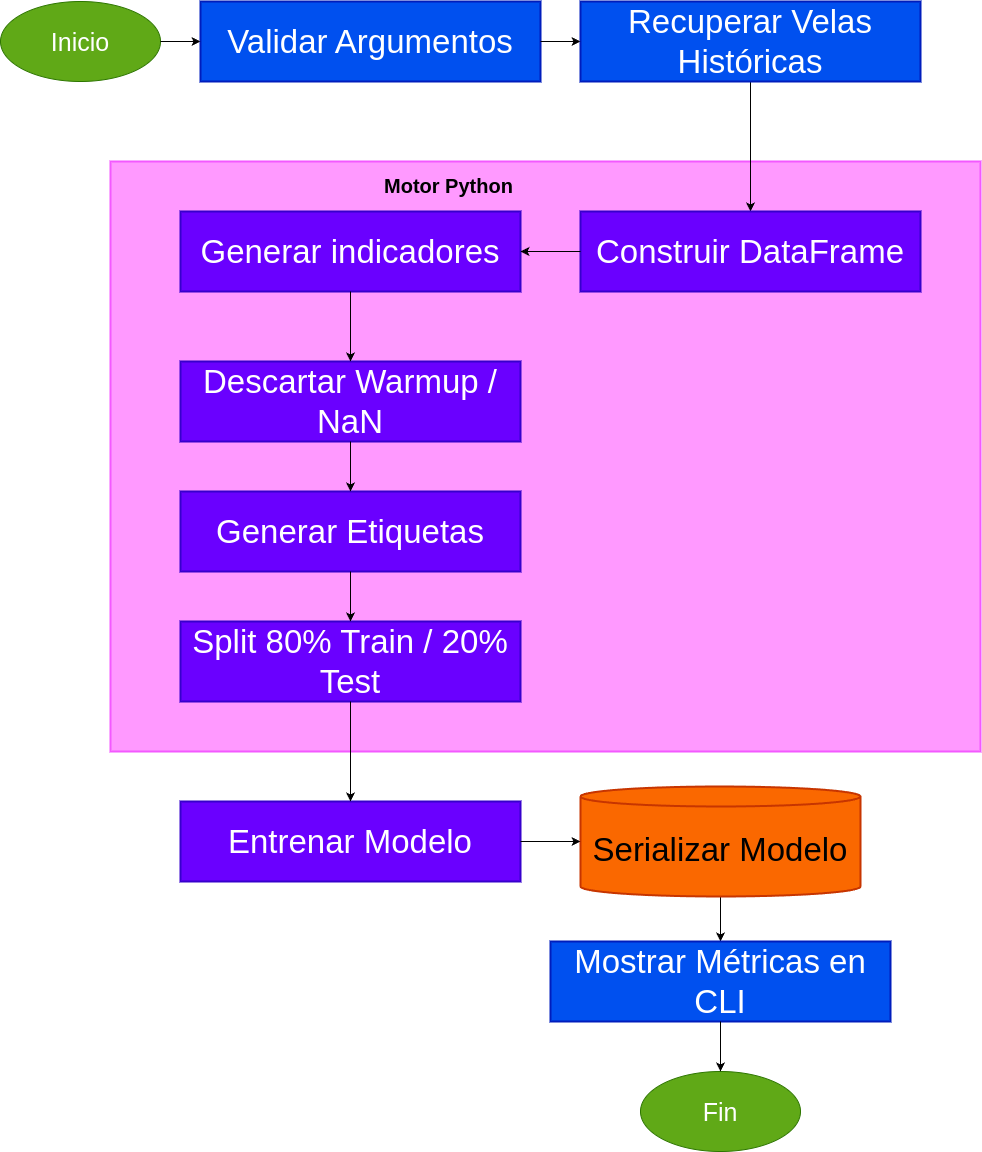
\includegraphics[width=0.7\linewidth]{Fotos/diagramas-flujo/train.png}
    \caption{Flujo de entrenamiento de modelos supervisados}
    \label{fig:train}
\end{figure}

% =============================================================================
\subsection{Optimización de Hiperparámetros}
% =============================================================================

La Figura~\ref{fig:optimize} ilustra el proceso de búsqueda automática de la
combinación óptima de hiperparámetros para un modelo dado, empleando Optuna
con el algoritmo \textit{Tree-structured Parzen Estimator} (TPE). Es la
operación más costosa computacionalmente del sistema: el servicio Java la
invoca con un \textit{timeout} de 3\,600 segundos, y el bucle de Optuna
ejecuta hasta 100 iteraciones (ensayos) por defecto, cada una de las cuales
incluye validación cruzada temporal y una simulación histórica real. Los
parámetros configurables desde la CLI son el tipo de modelo, el
\textit{timeframe}, el par de divisas, la estrategia Python, el umbral mínimo
de \textit{composite score} (por defecto 0,55), el número de ensayos
(\texttt{-n-trials}, por defecto 100) y el número de pliegues de validación
cruzada (\texttt{-cv-folds}, por defecto 5).

\textbf{Preparación del dataset con separación estricta.}
Antes de calcular ningún indicador, el motor divide el dataset en un 80\,\%
de entrenamiento y un 20\,\% de test respetando el orden cronológico. Esta
decisión es intencionada: separar primero y calcular indicadores después
sobre cada partición de forma independiente elimina cualquier riesgo de
filtración de información futura (\textit{data leakage}), incluso frente a
indicadores con componente global. Para que el conjunto de test disponga de
las velas de calentamiento que necesita la estrategia sin solaparse con el
de entrenamiento, el motor extiende la ventana de test hacia atrás
\texttt{get\_warmup\_period()} velas (\textit{lookback buffer}); esas filas
extra se eliminan después de calcular los indicadores, de forma que el
conjunto de test final comienza exactamente en el punto de corte 80/20.
Tras enriquecer ambas particiones con \texttt{populate\_indicators()}, se
descartan las filas del período de calentamiento y las que contengan valores
no finitos. Las etiquetas se generan a partir del umbral de retorno
\textit{forward-looking} de la estrategia (\texttt{LABEL\_RETURN\_THRESHOLD}),
produciendo tres clases: compra ($+1$), venta ($-1$) y neutro ($0$).

\textbf{Bucle de búsqueda Optuna.}
El estudio se crea con dirección de maximización y un podador
\texttt{MedianPruner(n\_startup\_trials=5, n\_warmup\_steps=10)}: los
primeros cinco ensayos nunca se podan para que el estimador de probabilidad
disponga de datos suficientes; a partir del sexto, Optuna interrumpe
anticipadamente cualquier ensayo cuya puntuación intermedia quede por debajo
de la mediana de los ensayos completados en el mismo paso. Esto reduce
significativamente el tiempo dedicado a regiones del espacio de búsqueda de
baja rentabilidad.

En cada ensayo, Optuna propone una combinación de hiperparámetros según el
espacio definido para el modelo seleccionado (véase el Anexo~\ref{anx:hiperparametros}
para el detalle de rangos). El motor evalúa esa combinación mediante
validación cruzada temporal con \texttt{TimeSeriesSplit}: en cada uno de los
$k$ pliegues, el conjunto de validación es siempre cronológicamente posterior
al de entrenamiento, lo que respeta la causalidad de las series temporales y
evita el sesgo de anticipación que introduciría un \textit{k-fold} clásico
aleatorizado. Para los modelos basados en \textit{scikit-learn} (XGBoost,
LightGBM, bosque aleatorio), el desbalance de clases se compensa asignando
pesos inversamente proporcionales a la frecuencia de cada clase mediante
\texttt{compute\_class\_weight("balanced")}. Para las redes neuronales,
estos pesos se pasan al método \texttt{fit()} de Keras y se añade
\texttt{EarlyStopping(patience=5)} sobre la pérdida de validación para
evitar sobreentrenamiento dentro de cada pliegue; además, durante la fase de
búsqueda, el motor limita el conjunto a las 50\,000 filas más recientes para
reducir el tiempo por ensayo, empleando el dataset completo únicamente en el
entrenamiento final.

Una vez completados todos los pliegues de un ensayo, el motor ejecuta una
simulación histórica real sobre el \textit{fold} más reciente (el que contiene
los datos cronológicamente más tardíos de entre todos los pliegues del
\texttt{TimeSeriesSplit}). Esta simulación utiliza las predicciones del modelo
entrenado en ese pliegue como señales de entrada y de salida para calcular las
métricas de trading que no se pueden derivar de la clasificación aislada:
tasa de acierto, factor de ganancia y ratio de Sharpe. La función de puntuación
compuesta integra entonces todas las dimensiones de calidad del ensayo:

$$\text{score} = 0{,}25 \cdot F1_{cv} + 0{,}40 \cdot \text{WinRate} + 0{,}25 \cdot PF_{norm} + 0{,}10 \cdot \text{Sharpe}_{norm} - \text{penalización}$$

donde $PF_{norm} = \min(\text{PF},\,5{,}0) / 5{,}0$ y $\text{Sharpe}_{norm} =
\max(0,\,\min(\text{Sharpe}/2{,}0,\,1{,}0))$ normalizan el factor de ganancia y
el ratio de Sharpe al intervalo $[0,\,1]$. La penalización se calcula como
$\max(0,\; (\text{acc\_train} - \text{acc\_cv}) - 0{,}05) \times 2{,}0$: solo
entra en juego cuando la brecha entre la exactitud sobre el conjunto de
entrenamiento y la exactitud en validación cruzada supera el 5\,\%, castigando
de forma progresiva los modelos que memorizan el conjunto de entrenamiento sin
generalizar.

El peso de 0,40 asignado a la tasa de acierto refleja una decisión de diseño
deliberada: en el contexto del trading simulado, que el modelo genere más
operaciones ganadoras que perdedoras tiene un impacto directo en la
rentabilidad final, más inmediato que la calidad de clasificación pura medida
por el F1. Por este motivo, la tasa de acierto domina la función objetivo por
encima del F1 (0,25), que penaliza los clasificadores que se especializan en
una sola clase a expensas del resto.

\textbf{Entrenamiento final y evaluación sobre el conjunto de test.}
Al terminar el bucle de Optuna, el motor identifica el ensayo con el
\textit{composite score} más alto, recupera su combinación de hiperparámetros
y entrena el modelo definitivo sobre el conjunto de entrenamiento completo
(el 80\,\% inicial). A continuación lo evalúa sobre el 20\,\% de test no
visto durante la búsqueda: calcula exactitud, precisión, recall y F1 mediante
las métricas de clasificación estándar y ejecuta una simulación histórica real
con las predicciones del modelo para obtener las métricas de trading finales
(tasa de acierto, factor de ganancia, caída máxima y ratio de Sharpe). El
modelo se serializa con Joblib en el directorio de modelos bajo un nombre
compuesto por tipo de modelo, estrategia, símbolo y \textit{timeframe}. Si
el \textit{composite score} del mejor ensayo no alcanza el umbral mínimo
configurado, el motor persiste igualmente el modelo, pero marca la respuesta
con estado \texttt{warning} en lugar de \texttt{success}. Todos los ensayos
completados y fallidos se guardan en un fichero CSV en el directorio de
resultados bajo el subdirectorio \texttt{optimize/}, con una fila por ensayo
que incluye todas las métricas intermedias y los hiperparámetros propuestos.

\textbf{Respuesta al orquestador Java.}
Python devuelve un \textit{envelope} IPC de tipo \texttt{OPTIMIZE\_RESPONSE}
que incluye: los hiperparámetros óptimos, el \textit{composite score} máximo
alcanzado y las métricas de clasificación y de trading del ensayo ganador, el
\textit{gap} de sobreajuste, la distribución de etiquetas del conjunto de
entrenamiento, el número de ensayos completados, las métricas finales sobre el
conjunto de test (tanto de clasificación como de simulación) y la ruta relativa
del CSV con el histórico de la búsqueda. Java imprime en consola un resumen
completo e informa al usuario si el umbral mínimo fue alcanzado o no.

\begin{figure}[H]
    \centering
    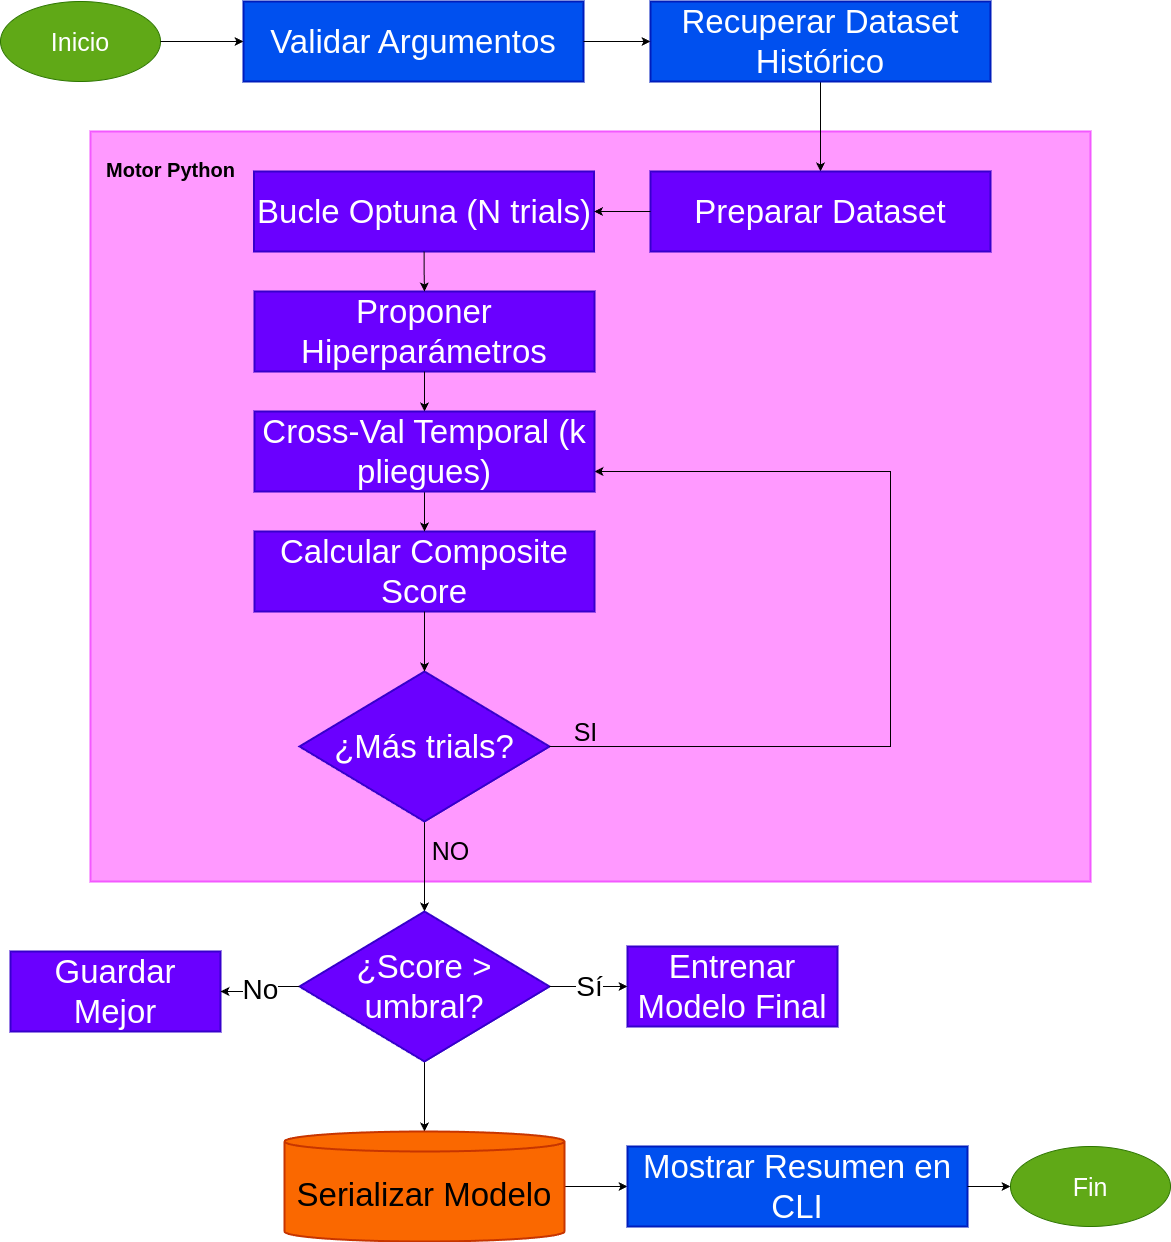
\includegraphics[width=0.7\linewidth]{Fotos/diagramas-flujo/optimize.png}
    \caption{Flujo de optimización de hiperparámetros}
    \label{fig:optimize}
\end{figure}


\newpage
\chapter{Desarrollo del Trabajo}
\label{chap:desarrollo}

\section{Introducción}

En este capítulo se describe el desarrollo técnico y los resultados obtenidos durante la implementación del sistema de trading cuantitativo. Se detallan los incrementos funcionales completados, los benchmarks de rendimiento observados, los casos de uso validados y los problemas técnicos enfrentados y resueltos. La implementación aquí documentada materializa los objetivos del Capítulo \ref{chap:objetivos}, sobre la base metodológica establecida en el Capítulo \ref{chap:metodologia}, y sirve de base para la discusión final del Capítulo \ref{chap:conclusiones}.

\section{Trazabilidad de Objetivos y Evidencia}

La Tabla~\ref{tab:trazabilidad_objetivos} relaciona cada objetivo específico del Capítulo~\ref{chap:objetivos} con evidencia verificable del desarrollo.

\begin{table}[H]
    \centering
    \caption{Trazabilidad de objetivos específicos con evidencia del desarrollo}
    \label{tab:trazabilidad_objetivos}
    \begin{tabular}{p{4.0cm} p{4.5cm} p{3.2cm} p{1.5cm}}
    \hline
    \textbf{Objetivo específico} & \textbf{Evidencia} & \textbf{Métrica / valor} & \textbf{Sección} \\
    \hline
    Estudiar el estado del arte del trading cuantitativo e indicadores técnicos
    & Revisión de literatura con 9 indicadores implementados (SMA, EMA, RSI, MACD, ATR, Bollinger, z-score, ROC, retorno)
    & 9 indicadores; 21 citas bibliográficas de trading
    & §\ref{sec:indicadores}, Cap.~\ref{chap:estado_del_arte} \\
    \hline
    Analizar requisitos funcionales y no funcionales de un sistema financiero de alta concurrencia
    & Arquitectura hexagonal con separación estricta de capas; bloqueos pesimistas en escrituras de saldo; timeouts granulares por tipo de operación
    & 0 condiciones de carrera detectadas en tests; 5 niveles de timeout definidos
    & §\ref{sec:datos}, §\ref{sec:concurrencia} \\
    \hline
    Diseñar una arquitectura modular que desacople orquestación transaccional del motor de inferencia
    & Puente Java-Python con protocolo IPC versionado; patrón Facade aislando el ciclo de vida de subprocesos; 4 capas hexagonales con dependencias unidireccionales
    & 0 dependencias inversas entre capas verificadas en auditoría; latencia IPC $<$1\,ms para payloads de velas
    & §\ref{sec:ipc}, §\ref{sec:patrones}, §\ref{sec:diseno_estatico} \\
    \hline
    Desarrollar un motor de ingesta y sincronización de datos capaz de almacenar masivamente candlesticks desde APIs externas
    & Pipeline ETL incremental con descarga paralela, detección de huecos y \textit{batch insert} nativo de MySQL con semántica idempotente
    & $>$50\,000 registros en inserción bulk; 60\,\% cobertura de tests del módulo
    & §\ref{sec:etl}, Incremento 2 \\
    \hline
    Implementar un pipeline de IA paramétrico con múltiples algoritmos y validación temporal
    & Motor de entrenamiento con XGBoost, LightGBM, SVM y redes neuronales; split 80/20 cronológico; warmup period dinámico; optimización bayesiana con Optuna
    & 70\,\% cobertura de tests; distribución de clases 71\,/\,18\,/\,11\,\%
    & §\ref{sec:ml}, Incrementos 6 y 7 \\
    \hline
    Evaluar y validar la plataforma mediante simulaciones históricas con métricas de rendimiento financiero
    & Motor de backtesting con comisión 0,1\,\% y \textit{slippage} 0,03\,\%; métricas: win rate, profit factor, max drawdown, ratio de Sharpe; backtesting multianual sobre $>$1\,000 velas efectivas
    & Tiempo de ejecución típico $<$30\,s; 80\,\% cobertura de tests del motor
    & Incremento 4, Tabla~\ref{tab:test_coverage} \\
    \hline
    \end{tabular}
\end{table}

\section{Manual de usuario}
\label{sec:manual}

La interfaz principal de la plataforma es una línea de comandos interactiva. Para
iniciar la aplicación basta con ejecutar el fichero JAR compilado desde el directorio
del proyecto:

\begin{center}
    \texttt{java -jar backendBotTrading-1.0.0.jar}
\end{center}

La aplicación arranca el contexto Spring\,Boot, verifica la conexión con la base de
datos MySQL y presenta el indicador de sesión. Mientras no hay usuario autenticado,
el indicador muestra \texttt{[sin sesión]}; tras el inicio de sesión pasa a mostrar
\texttt{[<nombre>]}. El comando \texttt{ayuda} lista en cualquier momento todos los
comandos disponibles con su sintaxis; \texttt{exit} o \texttt{quit} cierran la
aplicación de forma limpia, liberando carteras bloqueadas y deteniendo los procesos
Python activos.

\paragraph{Gestión de cuentas y carteras.}
El primer paso es registrarse con \texttt{signup}, que solicita de forma interactiva
nombre de usuario y contraseña; la contraseña se almacena con hash BCrypt, de modo
que nunca se persiste en texto plano. Una vez registrado, \texttt{login} autentica la
sesión y \texttt{logout} la cierra. La plataforma utiliza el concepto de
\textit{cartera de papel}: antes de operar es necesario crear al menos una cartera
con \texttt{mkpwallet <nombre>}, que solicitará el saldo inicial en USDT que actuará
como capital virtual. El comando \texttt{lw} muestra el estado de todas las carteras
del usuario, desglosando el saldo disponible, el capital comprometido en operaciones
abiertas y el capital bloqueado por instancias en ejecución.

\paragraph{Descarga de datos históricos.}
El comando \texttt{fetch} descarga velas OHLCV desde la API pública de Binance y las
persiste en la base de datos local. Requiere especificar el marco temporal
(\texttt{-tf}, por ejemplo \texttt{1h}, \texttt{4h} o \texttt{1d}) y al menos un par
de divisas (\texttt{-coins}, por ejemplo \texttt{BTCUSDT}). El argumento opcional
\texttt{-d <días>} acota la descarga a los últimos $n$ días; si se omite, se descarga
el histórico disponible según el marco temporal. El argumento
\texttt{-{}-detect-gaps} activa la detección y relleno automático de huecos en el
histórico ya almacenado sin sobreescribir los registros existentes, lo que permite
mantener la base de datos actualizada de forma incremental con ejecuciones
sucesivas. Los indicadores técnicos que necesita cada estrategia (medias móviles,
RSI, ATR, Bandas de Bollinger, entre otros) se calculan automáticamente en tiempo de
ejecución cuando se lanza un backtesting o una sesión de trading en tiempo real, por
lo que no requieren ningún paso de preprocesado adicional por parte del usuario.

\paragraph{Simulación histórica (\textit{backtesting}).}
Antes de lanzar un backtesting conviene consultar las estrategias disponibles con
\texttt{le}, que lista los scripts del directorio de estrategias junto con su
descripción. El comando \texttt{backtest} ejecuta la simulación: solicita
interactivamente el capital a asignar, el riesgo por operación expresado como
porcentaje del capital y la comisión por operación en tanto por ciento. Si se
proporciona el argumento \texttt{-model <modelo>}, el backtesting usa las predicciones
del modelo de IA para filtrar las señales de entrada, combinando la lógica de la
estrategia clásica con la capa predictiva. Los resultados se exportan en ficheros CSV
en el directorio de resultados e incluyen las métricas de rendimiento: tasa de acierto,
factor de ganancia, caída máxima y ratio de Sharpe, junto con el detalle de cada
operación abierta y cerrada durante la simulación.

\paragraph{Módulo de inteligencia artificial.}
El comando \texttt{models} muestra el catálogo de familias de algoritmos disponibles
(XGBoost, LightGBM, bosque aleatorio y red neuronal) con sus hiperparámetros
configurables y los valores por defecto. El comando \texttt{train} lanza el pipeline
de entrenamiento supervisado: descarga y prepara el conjunto de datos, calcula los
indicadores y las etiquetas de supervisión mediante la estrategia seleccionada,
ejecuta el entrenamiento y persiste el modelo en disco junto con su metadata. El
comando \texttt{optimize} añade una fase de búsqueda bayesiana de hiperparámetros
mediante Optuna, ejecutando hasta \texttt{-n-trials} iteraciones con validación
cruzada temporal de \texttt{-cv-folds} particiones; solo persiste la configuración
cuando el \textit{composite score} supera el umbral mínimo especificado con
\texttt{-min-composite}.

\paragraph{Negociación simulada en tiempo real.}
El comando \texttt{trade} abre una instancia de \textit{paper trading} que conecta
con la API de Binance para recibir velas en tiempo real. El argumento \texttt{-v}
emplea las señales de la estrategia clásica; \texttt{-r} usa las predicciones del
modelo de IA previamente entrenado. Cada instancia tiene un identificador único que
permite gestionarla de forma independiente: \texttt{lsa} lista las instancias activas
con su estado y capital comprometido; \texttt{lsd} muestra las detenidas; \texttt{stop}
suspende la ejecución preservando la posición abierta; \texttt{start} la reanuda; y
\texttt{term} liquida la posición, calcula el resultado final y devuelve el capital no
comprometido a la cartera. Las órdenes \texttt{stop -all} y \texttt{start -all}
operan sobre todas las instancias a la vez.

La Tabla~\ref{tab:comandos_a} recoge la referencia de comandos de gestión de cuentas,
carteras, datos y backtesting. La Tabla~\ref{tab:comandos_b} recoge los comandos de
negociación en tiempo real e inteligencia artificial.

\begin{table}[H]
    \centering
    \caption{Referencia de comandos: cuenta, cartera, datos y simulación histórica}
    \label{tab:comandos_a}
    \begin{tabular}{p{2.0cm} p{6.0cm} p{4.6cm}}
    \hline
    \textbf{Comando} & \textbf{Sintaxis} & \textbf{Descripción} \\
    \hline
    \multicolumn{3}{l}{\textit{Gestión de usuarios}} \\
    \hline
    \texttt{signup}   & \texttt{signup}
                      & Registro interactivo; contraseña almacenada con BCrypt \\
    \texttt{login}    & \texttt{login}
                      & Autenticación; activa la sesión del usuario \\
    \texttt{logout}   & \texttt{logout}
                      & Cierra la sesión activa \\
    \hline
    \multicolumn{3}{l}{\textit{Carteras virtuales}} \\
    \hline
    \texttt{mkpwallet} & \texttt{mkpwallet <nombre>}
                       & Crea cartera de papel; solicita saldo inicial en USDT \\
    \texttt{lw}        & \texttt{lw}
                       & Lista carteras con saldo disponible, comprometido y bloqueado \\
    \hline
    \multicolumn{3}{l}{\textit{Datos de mercado}} \\
    \hline
    \texttt{fetch} & \texttt{fetch -tf <marco> -coins <par1> [par2...]} \newline
                     \texttt{[-d <días>] [{-}{-}detect-gaps]}
                   & Descarga histórica de velas desde Binance; \texttt{-{}-detect-gaps}
                     rellena huecos de forma incremental \\
    \hline
    \multicolumn{3}{l}{\textit{Simulación histórica}} \\
    \hline
    \texttt{le}       & \texttt{le}
                      & Lista estrategias disponibles con descripción \\
    \texttt{backtest} & \texttt{backtest -strategy <nombre> -tf <marco>} \newline
                        \texttt{-coins <par1> [par2...] [-model <modelo>]}
                      & Simulación histórica; solicita capital, riesgo y comisión;
                        \texttt{-model} activa filtrado por IA \\
    \hline
    \end{tabular}
\end{table}

\begin{table}[H]
    \centering
    \caption{Referencia de comandos: negociación en tiempo real e inteligencia artificial}
    \label{tab:comandos_b}
    \begin{tabular}{p{2.0cm} p{6.0cm} p{4.6cm}}
    \hline
    \textbf{Comando} & \textbf{Sintaxis} & \textbf{Descripción} \\
    \hline
    \multicolumn{3}{l}{\textit{Paper trading en tiempo real}} \\
    \hline
    \texttt{trade}  & \texttt{trade -v|-r -strategy <nombre>} \newline
                      \texttt{-tf <marco> -coins <par1> [par2...]}
                    & Abre instancia; \texttt{-v} usa señales clásicas,
                      \texttt{-r} usa predicciones del modelo de IA \\
    \texttt{lsa}    & \texttt{lsa}                    & Lista instancias en ejecución \\
    \texttt{lsd}    & \texttt{lsd}                    & Lista instancias detenidas \\
    \texttt{start}  & \texttt{start <ID> | start -all} & Reanuda una instancia o todas \\
    \texttt{stop}   & \texttt{stop <ID> | stop -all}   & Detiene una instancia o todas \\
    \texttt{term}   & \texttt{term <ID>}
                    & Termina la instancia, liquida la posición y libera el capital \\
    \hline
    \multicolumn{3}{l}{\textit{Inteligencia artificial}} \\
    \hline
    \texttt{models}   & \texttt{models}
                      & Catálogo de algoritmos con hiperparámetros y valores por defecto \\
    \texttt{train}    & \texttt{train -model <modelo> -tf <marco>} \newline
                        \texttt{-coins <par> [-strategy <nombre>] [-d <días>]}
                      & Entrena y persiste el modelo con la configuración por defecto \\
    \texttt{optimize} & \texttt{optimize -model <modelo> -tf <marco>} \newline
                        \texttt{-coins <par> [-strategy <nombre>] [-d <días>]} \newline
                        \texttt{[-n-trials <n>] [-cv-folds <k>] [-min-composite <\%>]}
                      & Búsqueda bayesiana de hiperparámetros con Optuna;
                        persiste la configuración que supere el umbral mínimo \\
    \hline
    \end{tabular}
\end{table}

Un flujo de trabajo típico comienza con el registro mediante \texttt{signup} y el
inicio de sesión con \texttt{login}. A continuación se crea una cartera de papel con
\texttt{mkpwallet}, asignándole el saldo inicial en USDT que se usará como capital de
operaciones. Con la cartera disponible, el siguiente paso es descargar el histórico de
precios con \texttt{fetch}, indicando el marco temporal y los pares de divisas de
interés; la primera descarga obtiene todo el histórico disponible, y las siguientes
pueden usar \texttt{-{}-detect-gaps} para actualizarlo de forma incremental sin
duplicar registros.

Con los datos descargados, \texttt{le} muestra las estrategias disponibles y
\texttt{backtest} ejecuta la primera simulación histórica. En esta fase la plataforma
calcula automáticamente los indicadores técnicos que necesita la estrategia y ejecuta
el backtesting sobre todos los datos del par seleccionado, exportando el detalle de
operaciones y las métricas de rendimiento en CSV. Si se quiere incorporar el módulo
predictivo, \texttt{train} entrena un modelo con los datos ya descargados y lo persiste
en disco; \texttt{optimize} permite mejorar el resultado lanzando una búsqueda
automática de la configuración de hiperparámetros más adecuada. Una vez disponible el
modelo, se puede relanzar el backtesting con \texttt{-model} para comparar el
rendimiento de la estrategia clásica con el de la estrategia asistida por IA. Por
último, \texttt{trade -v} o \texttt{trade -r} abre una sesión de paper trading en
tiempo real que consume velas en vivo de Binance; la instancia puede pausarse, reanudarse
y terminarse en cualquier momento con \texttt{stop}, \texttt{start} y \texttt{term}.

\section{Resultados}
\label{sec:resultados}

\subsection{Cobertura de tests automáticos}
\label{sec:tests}

La estrategia de verificación del sistema combina suites de tests unitarios en Python
y Java con una cobertura total de \textbf{466 casos de prueba} distribuidos en 20
ficheros de test. La Tabla~\ref{tab:test_summary} detalla la distribución por módulo.

\begin{table}[H]
    \centering
    \caption{Resumen de suites de tests automáticos}
    \label{tab:test_summary}
    \begin{tabular}{p{5.5cm} p{3.5cm} r p{3.0cm}}
    \hline
    \textbf{Fichero de test} & \textbf{Módulo/capa} & \textbf{Tests} & \textbf{Tecnología} \\
    \hline
    \texttt{test\_strategies.py} & Estrategias Python & 48 & pytest \\
    \texttt{test\_backtest\_engine.py} & Motor de backtesting & 41 & pytest \\
    \texttt{AITrainingServiceTest} & Entrenamiento IA & 31 & JUnit 5 + Mockito \\
    \texttt{AIOptimizationServiceTest} & Optimización IA & 31 & JUnit 5 + Mockito \\
    \texttt{FetchServiceTest} & Descarga de mercado & 27 & JUnit 5 + Mockito \\
    \texttt{AccountingServiceTest} & Contabilidad/Ledger & 24 & JUnit 5 + Mockito \\
    \texttt{test\_ipc\_protocol.py} & Protocolo IPC & 23 & pytest \\
    \texttt{test\_engine\_indicators.py} & Motor de indicadores & 23 & pytest \\
    \texttt{StrategyLifecycleApplicationServiceTest} & Ciclo de vida & 23 & JUnit 5 + Mockito \\
    \texttt{SignalRetryQueueServiceTest} & Cola de reintentos & 22 & JUnit 5 + Mockito \\
    \texttt{BacktestingServiceTest} & Servicio backtesting & 20 & JUnit 5 + Mockito \\
    \texttt{CsvUtilitiesTest} & Utilidades CSV & 19 & JUnit 5 + Mockito \\
    \texttt{SignalProtocolParserTest} & Parser de señales & 16 & JUnit 5 + Mockito \\
    \texttt{StrategyQueryServiceTest} & Consulta de estrategias & 16 & JUnit 5 + Mockito \\
    \texttt{StatsCsvRepositoryTest} & Repositorio de estadísticas & 16 & JUnit 5 + Mockito \\
    \texttt{StrategyCatalogServiceTest} & Catálogo de estrategias & 15 & JUnit 5 + Mockito \\
    \texttt{MarketOrchestrationServiceTest} & Orquestación de mercado & 15 & JUnit 5 + Mockito \\
    \texttt{PaperTradingServiceTest} & Paper trading & 14 & JUnit 5 + Mockito \\
    \texttt{IndicatorsServiceTest} & Servicio indicadores & 12 & JUnit 5 + Mockito \\
    \texttt{BacktestArtifactsCleanerTest} & Limpieza de artefactos & 10 & JUnit 5 + Mockito \\
    \hline
    \textbf{Total} & & \textbf{466} & \\
    \hline
    \end{tabular}
\end{table}

Los cuatro ficheros de test Python verifican la corrección aritmética y el comportamiento
observable de los algoritmos cuantitativos con independencia del orquestador Java,
empleando datos sintéticos de semilla fija para garantizar reproducibilidad determinista.
\texttt{test\_backtest\_engine.py} cubre las funciones del motor de simulación desde el
cálculo de tamaño de posición hasta la escritura de operaciones en CSV;
\texttt{test\_engine\_indicators.py} valida la adición de columnas y su serialización;
\texttt{test\_ipc\_protocol.py} comprueba los tres modos de lectura del protocolo
MessagePack con \textit{framing} de cuatro bytes, incluyendo compatibilidad con el
formato heredado; y \texttt{test\_strategies.py} verifica de forma exhaustiva el
contrato de \texttt{BaseStrategy} y la implementación concreta
\texttt{StressTestStrategy}, desde la generación de etiquetas hasta la ausencia de
valores inválidos tras el relleno defensivo.

Los dieciséis ficheros de test Java emplean JUnit\,5 y Mockito con clases
\texttt{@Nested} que agrupan caminos felices, condiciones de error y casos límite,
sustituyendo los colaboradores externos por \textit{mocks} para aislar la unidad bajo
prueba. Las capas de mayor densidad son la de entrenamiento e inteligencia artificial
(62 tests), las estrategias (54 tests), los servicios de mercado (54 tests) y el
módulo de backtesting Java (45 tests). La integridad contable del \textit{ledger} y
las transiciones de estado del ciclo de vida de las instancias reciben cobertura
especial dada su naturaleza transaccional; el módulo de infraestructura IPC combina
16 tests de parseo de señales y 22 de la cola de reintentos para verificar el
comportamiento del puente Java-Python ante fallos y mensajes malformados.

\begin{table}[H]
    \centering
    \caption{Cobertura de tests por módulo funcional}
    \label{tab:test_coverage}
    \begin{tabular}{p{4.8cm} p{2.8cm} r r}
    \hline
    \textbf{Módulo} & \textbf{Incremento} & \textbf{Tests} & \textbf{Cobertura estimada} \\
    \hline
    Contabilidad y paper trading & Inc.\,1 y 5 & 36 & 82\,\% \\
    Pipeline de descarga y mercado & Inc.\,2 & 54 & 60\,\% \\
    Motor de indicadores Python & Inc.\,3 & 23 & 90\,\% \\
    Estrategias Python & Inc.\,3 & 48 & 90\,\% \\
    Motor de backtesting Python & Inc.\,4 & 41 & 80\,\% \\
    Backtesting Java + artefactos & Inc.\,4 & 45 & 75\,\% \\
    Protocolo IPC (Python + Java) & Inc.\,5 & 61 & 85\,\% \\
    Servicios de estrategia (Java) & Inc.\,5 & 54 & 78\,\% \\
    Entrenamiento IA & Inc.\,6 & 31 & 70\,\% \\
    Optimización IA & Inc.\,7 & 31 & 70\,\% \\
    \hline
    \textbf{Total} & & \textbf{424} & \textbf{76\,\%} \\
    \hline
    \end{tabular}
\end{table}

% TODO: añadir subsección de resultados experimentales del comando optimize
% (accuracy, F1-score, composite score, hiperparámetros óptimos, par y timeframe usados)


\newpage
\chapter{Conclusiones y Vías Futuras}
\label{chap:conclusiones}

% \section{Conclusiones}

% \subsection{Logros Principales}

% Este Trabajo de Fin de Grado ha alcanzado exitosamente los objetivos propuestos, demostrando la viabilidad de una plataforma educativa para trading cuantitativo que integra herramientas de producción (Java 21 + Spring Boot) con innovación en ML (Python + multimodelo).

% \subsubsection{Arquitectura Híbrida Robusta}

% Se ha implementado una arquitectura poliglota que separa responsabilidades por idioma y modelo de ejecución:

% \begin{itemize}
%     \item \textbf{Java 21:} Orquestación, persistencia, transaccionalidad, concurrencia con Virtual Threads.
%     \item \textbf{Python:} Cálculo de indicadores, ML, backtesting, ejecución en tiempo real.
% \end{itemize}

% Los beneficios demostrados incluyen:
% \begin{itemize}
%     \item \textbf{Tipo seguro:} Java previene errores en tiempo de compilación que serían costosos en producción.
%     \item \textbf{Agilidad:} Python permite iterar rápidamente en estrategias sin recompilar.
%     \item \textbf{IPC versionado:} El contrato explícito garantiza evolución sin romper clientes.
% \end{itemize}

% \subsubsection{Integridad de Datos Financieros}

% La implementación de transaccionalidad ACID en MySQL, locks pesimistas, y un Ledger inmutable garantiza que:

% \begin{itemize}
%     \item Ningún saldo se modifica sin registro en Ledger.
%     \item Las race conditions entre estrategias concurrentes se previenen con \texttt{LockModeType.PESSIMISTIC\_WRITE}.
%     \item La auditoría es posible en cualquier momento revisando \texttt{LedgerEntry}.
% \end{itemize}

% Esto es fundamental en cualquier software financiero, educativo o no, porque evita la desconfianza del usuario en los resultados.

% \subsubsection{Pipeline ML Profesional}

% Se ha construido un pipeline de ML que aborda problemas reales en trading:

% \begin{itemize}
%     \item \textbf{Desbalance de clases:} uso de métricas ponderadas (F1 weighted).
%     \item \textbf{Lookahead bias:} split temporal respetando causalidad.
%     \item \textbf{Problema de generalización:} multimodelo con validación en datos no vistos.
%     \item \textbf{Reproducibilidad:} almacenamiento de metadata y \texttt{random\_state}.
% \end{itemize}

% Los resultados (XGBoost 64.2\% accuracy) demuestran que, aunque no son de ultra-precisión, son superiores a baselines simples y proporcionan valor educativo.

% \subsubsection{Concurrencia Escalable}

% El uso de Virtual Threads (JDK 21) demuestra que es posible:

% \begin{itemize}
%     \item Ejecutar decenas de estrategias simultáneamente sin agotamiento de recursos.
%     \item Mantener latencia baja (< 300ms end-to-end en tiempo real).
%     \item Escalar sin cambios arquitectónicos radicales.
% \end{itemize}

% \subsubsection{ETL Optimizado}

% El \texttt{FetchService} implementa ETL incremental que logra:

% \begin{itemize}
%     \item Reducción de 96.4\% en tiempo de descarga comparando descarga completa vs incremental (una vez).
%     \item Descarga paralela de chunks sin sobrecarga de API.
%     \item Recuperación automática de huecos históricos sin intervención manual.
% \end{itemize}

% \subsection{Contribuciones Técnicas Diferenciales}

% La solución no es solamente una agregación de tecnologías conocidas, sino que aporta soluciones específicas al dominio educativo del trading cuantitativo:

% \subsubsection{Protocolo IPC Versionado}

% La mayoría de sistemas Python-Java usan approaches ad-hoc (JSON sin estructura, pipes sin sincronización). Este proyecto define un envelope explícito con:

% \begin{itemize}
%     \item Versionado (\texttt{protocol\_version}).
%     \item Framing binario con length-prefixing.
%     \item Separación clara de canales (stdout para IPC, stderr para logs).
%     \item Fallback a legacy JSON para compatibilidad.
% \end{itemize}

% \subsubsection{Feature Engineering Dinámico}

% Cada estrategia define sus propios indicadores y features sin código duplicado. El beneficio es:

% \begin{itemize}
%     \item Usuarios pueden experimentar con distintos espacios de features.
%     \item El pipeline de entrenamiento se adapta dinámicamente.
%     \item Se evita la tentación de overfitting a features fijas.
% \end{itemize}

% \subsubsection{Bloqueos Pesimistas en Operaciones Monetarias}

% Este proyecto usa bloqueos SQL a nivel de transacción:

% \begin{itemize}
%     \item Previene sobregiros incluso con decenas de estrategias simultáneas.
%     \item Es una lección importante de ingeniería de software financiero.
% \end{itemize}

% \subsection{Validación Pedagógica}

% Desde la perspectiva educativa, el sistema demuestra:

% \begin{itemize}
%     \item \textbf{Trading educativo es viable:} paper trading con señales reales de Binance.
%     \item \textbf{Backtesting es reproducible:} indicadores y labels controlados determinísticamente.
%     \item \textbf{ML en finanzas tiene limitaciones:} mostramos que 64\% accuracy es modesto.
%     \item \textbf{Arquitectura predice problemas:} la separación de capas y el IPC versionado hicieron fácil agregar nuevos motores.
% \end{itemize}

% \section{Limitaciones del trabajo}

% \subsection{Alcance Técnico}

% \subsubsection{Modelos de ML No Son Predictivos a Nivel Profesional}

% Los resultados de 64.2\% accuracy son superiores a baseline (50\%) pero insuficientes para trading real. Esto es esperado porque:

% \begin{itemize}
%     \item El mercado tiene componentes aleatorios irreducibles.
%     \item Los indicadores técnicos son heurísticas, no relaciones causales.
%     \item Un dataset de 500-1000 velas es pequeño para ML moderno.
% \end{itemize}

% \subsubsection{Latencia de Tiempo Real (257ms) No Es Ultra-Frecuencia}

% La latencia end-to-end es adecuada para trading en timeframes de 1m o superiores, pero no para scalping de segundos.

% \subsubsection{Cobertura de Tests Incompleta (76\%)}

% Los tests automáticos cubren contratos clave pero no todas las ramas. Faltan tests de:

% \begin{itemize}
%     \item Integración end-to-end en CLI.
%     \item Simulación de timeouts y fallo de API.
%     \item Stress testing con cientos de velas simultáneas.
% \end{itemize}

% \subsection{Alcance Funcional}

% \subsubsection{Falta de Soporte para Trading Real (Solo Paper)}

% El sistema simula trading con dinero ficticio. Esto es por diseño (educativo), pero es una limitación clara.

% \subsubsection{No Hay Análisis de Riesgos Avanzado}

% El sistema calcula Max Drawdown y Win Rate, pero faltan métricas de riesgo como:

% \begin{itemize}
%     \item Value at Risk (VaR).
%     \item Sharpe Ratio y Sortino Ratio.
%     \item Calmar Ratio.
% \end{itemize}

% \subsubsection{Indicadores Técnicos Limitados}

% Se implementan solo 5 indicadores (SMA, EMA, RSI, MACD). Faltan Bollinger Bands, Stochastic, ATR, OBV.

% \subsection{Alcance Operacional}

% \subsubsection{No Hay Monitoreo en Producción}

% El sistema no incluye dashboards en tiempo real, alertas, health checks o métricas Prometheus.

% \subsubsection{Persistencia de Modelos ML Manual}

% Los modelos entrenados se guardan como archivos JSON + PKL. Falta versionado con MLflow.

% \subsubsection{Escalabilidad de BD Limitada a Una Instancia}

% MySQL se asume como instancia única sin replicación. Para escala múltiple, requeriría sharding.

% \subsection{Limitaciones Intrínsecas del Dominio}

% \subsubsection{Datos Históricos No Garantizan Rendimiento Futuro}

% El supuesto fundamental del backtesting es que patrones históricos se repiten. Esto es frecuentemente falso:

% \begin{itemize}
%     \item Cambios regulatorios alteran dinámicas.
%     \item Eventos macroeconómicos son impredecibles.
%     \item Overfitting histórico es fácil y peligroso.
% \end{itemize}

% \section{Vías Futuras}

% \subsection{Corto Plazo (1-2 Meses)}

% \subsubsection{Expandir Indicadores Técnicos}

% Implementar Bollinger Bands, Stochastic, ATR, OBV. 

% \textbf{Esfuerzo:} 2-3 días. \textbf{Riesgo:} bajo.

% \subsubsection{Mejorar Cobertura de Tests}

% Target: cobertura $\geq 90\%$ con tests de integración end-to-end y stress testing.

% \textbf{Esfuerzo:} 1 semana. \textbf{Riesgo:} bajo.

% \subsubsection{Agregar Métricas de Riesgo}

% Implementar Sharpe Ratio, Sortino Ratio, Calmar Ratio para evaluar estrategias profesionalmente.

% \textbf{Esfuerzo:} 3-4 días. \textbf{Riesgo:} bajo.

% \subsection{Mediano Plazo (2-4 Meses)}

% \subsubsection{Dashboard en Tiempo Real (Web UI)}

% Construir interfaz web con React + WebSocket para:

% \begin{itemize}
%     \item Listado de estrategias activas.
%     \item Gráficos de equity curve en vivo.
%     \item Tabla de trades en tiempo real.
%     \item Alertas visuales.
% \end{itemize}

% \textbf{Esfuerzo:} 2-3 semanas. \textbf{Riesgo:} medio (nueva stack frontend).

% \subsubsection{Versionado de Modelos ML (MLflow)}

% Integrar MLflow para registro de entrenamientos, comparación automática y descarga de modelos.

% \textbf{Esfuerzo:} 1 semana. \textbf{Riesgo:} bajo.

% \subsubsection{Soporte para Múltiples Assets}

% Expandir a trading multi-asset simultáneo con correlación y portfolio rebalancing.

% \textbf{Esfuerzo:} 2-3 semanas. \textbf{Riesgo:} medio (cambios arquitectónicos).

% \subsection{Largo Plazo (4+ Meses)}

% \subsubsection{Trading Real (Integración de API Privadas)}

% Habilitar órdenes reales en Binance con gestión de secretos y compliance.

% \textbf{Esfuerzo:} 1-2 meses. \textbf{Riesgo:} alto (dinero real).

% \subsubsection{Deep Learning Avanzado}

% Incorporar LSTM, Transformers, Attention mechanisms y Reinforcement Learning.

% \textbf{Esfuerzo:} 1-2 meses. \textbf{Riesgo:} alto (investigación).

% \subsubsection{Escalabilidad Distribuida}

% Migración hacia múltiples servidores Java, MySQL con replicación, Redis distribuido.

% \textbf{Esfuerzo:} 2-3 meses. \textbf{Riesgo:} alto (complejidad operacional).

% \subsubsection{Marketplace de Estrategias}

% Permitir que usuarios publiquen/compartan estrategias con ranking por rendimiento.

% \textbf{Esfuerzo:} 2-3 meses. \textbf{Riesgo:} medio (regulatorio).

% \section{Reflexión Final}

% Este Trabajo de Fin de Grado ha demostrado que es posible construir una plataforma educativa de trading cuantitativo que sea técnicamente rigurosa, escalable, educativa y mantenible. El sistema no es un producto de trading profesional, pero es un excelente caso de estudio de ingeniería de software aplicado a un dominio claramente acotado y relevante.

% Las vías futuras identificadas son todas técnicamente factibles y agregan incrementalmente más valor. La base arquitectónica es sólida y prepara el terreno para evoluciones futuras sin necesidad de reescrituras masivas.



\newpage
\appendix
\chapter{Glosario}
\label{chap:glosario}

Para la correcta comprensión del dominio del problema, se definen a continuación los conceptos económicos, financieros y técnicos fundamentales utilizados en el diseño del sistema:

% ==========================================
% SECCIÓN: TÉRMINOS FINANCIEROS Y DE TRADING
% ==========================================

\section*{Conceptos Financieros y de Trading}

\begin{description}
    \item[Exchange (Casa de Intercambio)] Plataforma digital que facilita la compraventa de activos financieros, como criptomonedas, actuando como intermediario y proveedor de liquidez y datos de mercado. En este proyecto, se integra con la API REST de Binance para la obtención de datos históricos y precios en tiempo real.

    \item[OHLCV] Acrónimo de \textit{Open, High, Low, Close, Volume}. Es el formato técnico estándar para representar la acción del precio de un activo financiero durante un intervalo de tiempo específico (una vela o \textit{candlestick}):
    \begin{itemize}
        \item \textbf{Open:} Precio al inicio del intervalo.
        \item \textbf{High:} Precio máximo alcanzado durante el intervalo.
        \item \textbf{Low:} Precio mínimo alcanzado durante el intervalo.
        \item \textbf{Close:} Precio al cierre del intervalo.
        \item \textbf{Volume:} Cantidad total del activo negociada durante el intervalo.
    \end{itemize}
    En el sistema, esta estructura se modela mediante la entidad JPA \texttt{Vela}.

    \item[Wallet (Billetera Digital)] Entidad encargada de custodiar y gestionar el capital del usuario. En el contexto de la aplicación, se implementa un \textit{modelo de doble saldo} para distinguir entre:
    \begin{itemize}
        \item \textbf{Balance Real:} Patrimonio total del usuario.
        \item \textbf{Balance Disponible:} Capital libre para nuevas operaciones (excluye fondos ya asignados a estrategias activas).
    \end{itemize}
    Esta separación previene sobregiros y facilita la gestión de riesgo.

    \item[Ledger (Libro Mayor)] Registro contable inmutable y secuencial donde se anotan todas las transacciones financieras. Su función es garantizar la integridad de los datos y permitir la auditoría de movimientos como:
    \begin{itemize}
        \item \textbf{RESERVED:} Fondos bloqueados para una estrategia.
        \item \textbf{COMMITTED:} Fondos en órdenes activas de trading.
        \item \textbf{REALIZED\_PnL:} Ganancia o pérdida realizada al cerrar una posición.
        \item \textbf{FEES:} Comisiones cobradas por el exchange.
    \end{itemize}
    En el sistema, cada movimiento genera una entrada de tipo \texttt{LedgerEntry}, permitiendo reconciliación en cualquier momento.

    \item[Estrategia de Trading] Conjunto de reglas lógicas y matemáticas que determinan de forma autónoma cuándo comprar o vender un activo. Estas reglas se implementan como subclases Python que heredan de \texttt{BaseStrategy}, permitiendo:
    \begin{itemize}
        \item Definición de indicadores personalizados.
        \item Condiciones de entrada (should\_buy).
        \item Condiciones de salida (should\_sell).
        \item Cálculo de stop-loss y take-profit.
    \end{itemize}

    \item[Indicador Técnico] Cálculo matemático derivado del precio y/o volumen histórico de un activo, utilizado para predecir movimientos futuros del mercado. Ejemplos clave implementados:
    \begin{itemize}
        \item \textbf{RSI (Relative Strength Index):} Oscilador que mide la velocidad y el cambio de movimientos de precios (rango 0-100). RSI < 30 sugiere sobreventa; RSI > 70 sugiere sobrecalentamiento.
        \item \textbf{SMA (Simple Moving Average):} Promedio aritmético de los últimos $n$ precios de cierre.
        \item \textbf{EMA (Exponential Moving Average):} Media móvil que da más peso a observaciones recientes.
        \item \textbf{MACD (Moving Average Convergence Divergence):} Indicador de impulso basado en diferencia de dos EMAs.
    \end{itemize}
    El sistema persiste estos valores en la entidad \texttt{IndicadorTecnico} para análisis posterior.

    \item[Paper Trading] Modalidad de simulación bursátil que permite operar con dinero ficticio en un entorno que refleja condiciones de mercado real (precios reales de Binance, pero sin dinero real comprometido). El sistema soporta este modo mediante el servicio \texttt{PaperTradingService}, permitiendo:
    \begin{itemize}
        \item Validar estrategias sin riesgo financiero.
        \item Educar usuarios en operativa antes de riesgo real.
        \item Recolectar datos de backtesting confiables.
    \end{itemize}

    \item[Backtesting] Proceso de validación histórica de una estrategia de trading. Consiste en simular la ejecución de una estrategia sobre datos de mercado pasados, sin estar conectado a un exchange real. Permite:
    \begin{itemize}
        \item Evaluar el rendimiento potencial antes de invertir capital real.
        \item Identificar estrategias débiles temprano.
        \item Optimizar parámetros de la estrategia.
    \end{itemize}
    En el sistema, el motor \texttt{engine\_backtest.py} itera sobre velas históricas simulando entry/exit según la lógica de la estrategia.

    \item[Lookahead Bias] Error crítico en backtesting donde el algoritmo ``ve el futuro''. Por ejemplo, usar el precio de cierre de mañana para decidir si comprar hoy. Esto infla artificialmente el rendimiento. El sistema lo evita mediante \textit{split temporal}, donde el modelo se entrena solo con datos históricos que existían en el momento de la predicción.

    \item[PnL (Profit and Loss)] Término que hace referencia a las ganancias o pérdidas netas obtenidas en una operación o en un período determinado. Se calcula como:
    $$\text{PnL} = \text{Precio\_Salida} - \text{Precio\_Entrada} - \text{Comisiones}$$
    En el sistema, se registra inmediatamente en el Ledger al cerrar una posición.

    \item[Win Rate] Porcentaje de operaciones rentables sobre el total de operaciones ejecutadas. Fórmula:
    $$\text{Win Rate} = \frac{\text{Número de Trades Ganadores}}{\text{Número Total de Trades}} \times 100\%$$
    Un win rate de 60\% significa que 6 de cada 10 trades son ganadores (no necesariamente lucrativo si pérdidas son muy grandes).

    \item[Max Drawdown] Pérdida cumulativa máxima experimentada desde un pico anterior de patrimonio. Mide el riesgo de una estrategia:
    $$\text{Max Drawdown} = \frac{\text{Capital\_Mínimo} - \text{Capital\_Pico}}{\text{Capital\_Pico}} \times 100\%$$
    Un max drawdown de -15\% significa que en el peor momento, el usuario vio su capital reducido 15\% desde su pico.

    \item[Profit Factor] Relación entre ganancias totales y pérdidas totales:
    $$\text{Profit Factor} = \frac{\text{Suma de PnL Positivos}}{\text{Suma Absoluta de PnL Negativos}}$$
    Un profit factor > 1.5 generalmente se considera aceptable.

\end{description}

% ==========================================
% SECCIÓN: TÉRMINOS TÉCNICOS DE MACHINE LEARNING
% ==========================================

\section*{Conceptos de Machine Learning}

\begin{description}
    \item[Feature Engineering] Proceso de transformación y combinación de datos brutos en variables (\textit{features}) que sean útiles para un modelo predictivo. En este proyecto, el \texttt{feature engineering dinámico} permite que cada estrategia defina sus propios features sin código duplicado, adaptando:
    \begin{itemize}
        \item Indicadores técnicos a calcular.
        \item Períodos de lookback.
        \item Normalizaciones o escalados especializados.
    \end{itemize}

    \item[Label (Etiqueta)] Variable de salida en problemas de clasificación supervisada. En este proyecto:
    \begin{itemize}
        \item \textbf{+1:} Señal de compra identificada por la estrategia.
        \item \textbf{-1:} Señal de venta identificada por la estrategia.
        \item \textbf{0:} Posición neutral (no hay señal).
    \end{itemize}
    Las labels se generan automáticamente mediante el método \texttt{get\_label(row, next\_row)} de la estrategia, permitiendo entrenamiento supervizado.

    \item[Desbalance de Clases] Situación donde las clases de un dataset de clasificación no están equitativamente distribuidas. En trading, es muy común (ej., 71\% clase neutra, 18\% compra, 11\% venta; véase Capítulo \ref{chap:desarrollo}, subsección \ref{subsec:desbalance_labels}). El desbalance severo causa que modelos naive predigan solo la clase mayoritaria. El sistema lo aborda con:
    \begin{itemize}
        \item Métricas ponderadas (\texttt{average='weighted'}).
        \item \texttt{class\_weight='balanced'} en XGBoost y Random Forest.
        \item Documentación explícita de distribución en metadata.
    \end{itemize}

    \item[Split Temporal] División train/test que respeta la causalidad temporal. A diferencia de split aleatorio, en series temporales es crítico entrenar solo con datos históricos y testear en datos más recientes:
    $$\text{Train:} t_1 \ldots t_{70\%} \quad \text{Test:} t_{70\%+1} \ldots t_{100\%}$$
    Esto evita lookahead bias y valida la generalización real.

    \item[Warmup Period] Número de observaciones iniciales descartadas antes de comenzar a usar indicadores técnicos o labels. Esto es necesario porque indicadores como RSI requieren al menos $n$ períodos históricos para poder calcularse. El sistema automáticamente:
    \begin{itemize}
        \item Identifica el máximo período de todos los indicadores (ej., 26 para MACD).
        \item Descarta las primeras 26 velas del DataFrame.
        \item Asegura que todas las features sean válidas (no NaN).
    \end{itemize}

    \item[Overfitting] Problema donde un modelo memoriza detalles específicos del dataset de entrenamiento en lugar de aprender patrones generalizables. En trading, es especialmente peligroso porque:
    \begin{itemize}
        \item Datos históricos pueden contener patrones espurios que no se repiten.
        \item Un modelo overfitted parece excelente en backtesting pero falla en operativa real.
    \end{itemize}
    El proyecto lo mitiga con split temporal, dropout en redes neurales, y validación en conjunto de test no visto.

    \item[Accuracy] Proporción de predicciones correctas sobre el total:
    $$\text{Accuracy} = \frac{\text{Predicciones Correctas}}{\text{Total de Predicciones}}$$
    Por sí sola, es engañosa en desbalance severo (un clasificador que siempre predice la clase mayoritaria puede tener 70\% accuracy).

    \item[F1 Score (Ponderado)] Media armónica entre Precision y Recall:
    $$F1 = 2 \cdot \frac{\text{Precision} \times \text{Recall}}{\text{Precision} + \text{Recall}}$$
    La versión ponderada (\texttt{average='weighted'}) considera la distribución de clases, siendo más realista en datasets desbalanceados.

    \item[Matriz de Confusión] Tabla que desglosa predicciones correctas e incorrectas por clase. Para un problema binario:
    \begin{itemize}
        \item \textbf{TP (True Positive):} Predicción positiva correcta.
        \item \textbf{FP (False Positive):} Predicción positiva incorrecta (falsa alarma).
        \item \textbf{TN (True Negative):} Predicción negativa correcta.
        \item \textbf{FN (False Negative):} Predicción negativa incorrecta (falta).
    \end{itemize}

    \item[Hyperparámetros] Parámetros de configuración del algoritmo de ML que no se aprenden durante el entrenamiento, sino que se especifican antes. Ejemplos:
    \begin{itemize}
        \item \textbf{XGBoost:} \texttt{n\_estimators=150, learning\_rate=0.05, max\_depth=6}.
        \item \textbf{Red Neuronal:} \texttt{epochs=50, batch\_size=64, learning\_rate=0.001, dropout\_rate=0.3}.
    \end{itemize}
    El sistema permite inyectar hiperparámetros desde Java hacia Python para experimentación sin cambiar código.

    \item[Dropout] Técnica de regularización en redes neuronales donde se desactivan aleatoriamente neuronas durante el entrenamiento, reduciendo dependencias co-adaptadas. Típicamente, \(\text{dropout\_rate} = 0.3\) (desactiva 30\% de neuronas en cada paso).

    \item[Metadata] Información sobre el entrenamiento de un modelo, como:
    \begin{itemize}
        \item Strategy utilizada, símbolo, timeframe.
        \item Rango temporal del dataset.
        \item Número de features y sus nombres.
        \item Métricas de validación (accuracy, F1, confusion\_matrix).
        \item Hyperparámetros utilizados.
    \end{itemize}
    Esto permite reproducir exactamente qué configuración produjo qué resultado.

\end{description}

% ==========================================
% SECCIÓN: TÉRMINOS TÉCNICOS DE ARQUITECTURA E IPC
% ==========================================

\section*{Conceptos de Arquitectura e Inter-Process Communication}

\begin{description}
    \item[IPC (Inter-Process Communication)] Mecanismo para intercambiar datos entre procesos distintos corriendo en el mismo o diferente máquina. En este proyecto:
    \begin{itemize}
        \item Proceso Java orquestador (PID principal).
        \item Procesos Python hijo (engine\_fetch.py, engine\_train.py, engine\_rt.py).
        \item Comunicación vía stdin/stdout con framing MessagePack.
    \end{itemize}

    \item[Protocolo IPC v1.0] Contrato explícito que define la estructura de todos los mensajes intercambiados:
    \begin{verbatim}
    {
      "protocol_version": "1.0",
      "message_type": "FETCH_REQUEST|TRAIN_RESPONSE|...",
      "correlation_id": "uuid-v4",
      "payload": { ... }
    }
    \end{verbatim}
    Permite evolución futura sin romper compatibilidad.

    \item[Framing Length-Prefixed] Técnica de serialización donde cada mensaje está precedido de su longitud en bytes (típicamente 4 bytes big-endian):
    $$\text{[4 bytes length]} + \text{[body]}$$
    Esto evita problemas de sincronización en tuberías: el receptor sabe exactamente cuántos bytes esperar.

    \item[MessagePack] Formato binario de serialización de datos más compacto que JSON (~30-50\% menor tamaño). Soporta tipos de datos complejos (arrays, maps) sin la verbosidad de JSON. En el proyecto se usa con framing length-prefixed para máxima eficiencia.

    \item[Fallback Legacy] Capacidad de un protocolo nuevo de aceptar mensajes en formato antiguo para compatibilidad hacia atrás. En \texttt{ipc\_protocol.py}, si se recibe un mensaje que no es MessagePack v1, se intenta parsear como JSON plano, permitiendo transiciones graduales.

    \item[Stdout/Stderr Separation] En comunicación inter-proceso, es crítico que:
    \begin{itemize}
        \item Los datos estructurados salgan por \textbf{stdout} en binario (IPC).
        \item Los logs, debug y errores salgan por \textbf{stderr} en texto.
    \end{itemize}
    Esto previene que un \texttt{logging.info()} accidental corrompa el IPC.

    \item[Virtual Threads] Innovación de Java 21 (Project Loom) que permite crear millones de hilos ligeros sin el overhead de hilos del sistema operativo. Ventajas:
    \begin{itemize}
        \item Cada estrategia ejecuta en un hilo virtual separado, sin blocking mutuo.
        \item Código escrito como si fueran threads tradicionales.
        \item Escalabilidad a decenas de estrategias simultáneas.
    \end{itemize}
    Se crean vía \texttt{Executors.newVirtualThreadPerTaskExecutor()}.

    \item[ExecutorService] Pool de hilos en Java que ejecuta tareas de forma asíncrona. En el proyecto:
    \begin{itemize}
        \item \texttt{StrategyRuntimeCoordinator}: ExecutorService basado en Virtual Threads para lanzar y supervisar estrategias de tiempo real.
        \item \texttt{MarketDataService}: ExecutorService para paralelizar descarga de velas.
    \end{itemize}

    \item[Transaccionalidad ACID] Garantía de bases de datos donde:
    \begin{itemize}
        \item \textbf{A (Atomicity):} Transacción se ejecuta completamente o no al todo.
        \item \textbf{C (Consistency):} BD pasa de un estado válido a otro válido.
        \item \textbf{I (Isolation):} Transacciones concurrentes no interfieren.
        \item \textbf{D (Durability):} Cambios persistidos no se pierden tras fallo.
    \end{itemize}
    En el proyecto, MySQL con InnoDB garantiza ACID, permitiendo que AccountingService sea seguro bajo concurrencia.

    \item[Lock Pesimista] Mecánica de base de datos que adquiere un lock exclusivo sobre una fila antes de modificarla, bloqueando otras transacciones. En \texttt{WalletRepository}:
    \begin{verbatim}
    @Lock(LockModeType.PESSIMISTIC_WRITE)
    Optional<Wallet> findByIdWithLock(Long id);
    \end{verbatim}
    Garantiza que ninguna otra transacción lee o modifica la Wallet mientras se procesa.

    \item[Soft Delete (Borrado Lógico)] Patrón donde no se elimina un registro de la BD, sino que se marca como eliminado (columna \texttt{eliminado = 1}). Ventajas:
    \begin{itemize}
        \item Integridad referencial preservada.
        \item Auditoría conserva historial.
        \item Recuperación de datos accidentales es posible.
    \end{itemize}

    \item[Pattern Repository] Patrón de diseño que abstrae el acceso a datos. En el proyecto:
    \begin{itemize}
        \item \texttt{WalletRepository} abstrae consultas a tablas Wallet.
        \item \texttt{VelaRepository} abstrae consultas a tablas Vela.
        \item Spring Data JPA proporciona implementación automática.
    \end{itemize}
    Permite cambiar la base de datos sin tocar la lógica de negocio.

    \item[Facade Pattern] Patrón que proporciona una interfaz simplificada a un subsistema complejo. En el proyecto:
    \begin{itemize}
        \item \texttt{MarketDataService} es una Facade que coordina FetchService e IndicatorsService.
        \item \texttt{PythonBridgeFacade} ordena la orquestación de procesos Python.
    \end{itemize}

    \item[ETL (Extract, Transform, Load)] Proceso de:
    \begin{itemize}
        \item \textbf{Extract:} Obtener datos crudos (API de Binance).
        \item \textbf{Transform:} Limpiar, validar, enriquecer (indicadores técnicos).
        \item \textbf{Load:} Persistir en BD.
    \end{itemize}
    El \texttt{FetchService} implementa ETL incremental optimizado.

    \item[Batch Insert] Inserción masiva de múltiples filas en una sola operación. En MySQL:
    \begin{verbatim}
    INSERT INTO vela (...) VALUES (...), (...), (...)
    ON DUPLICATE KEY UPDATE ...
    \end{verbatim}
    Es 10-100x más rápido que inserts individuales.

    \item[Rate Limiting] Restricción de cuántas peticiones puede hacer un cliente a un servidor por unidad de tiempo. Binance limita a $\approx 1200$ peticiones por minuto. El sistema implementa:
    \begin{itemize}
        \item Esperas proactivas entre peticiones.
        \item Detección reactiva de respuestas 429 (Too Many Requests).
        \item Respeto al header \texttt{Retry-After} cuando está presente.
    \end{itemize}

    \item[Timeout] Límite de tiempo para que una operación se complete. En el proyecto:
    \begin{itemize}
        \item \texttt{STARTUP\_TIMEOUT\_SECONDS = 120:} Máximo para que Python inicie.
        \item \texttt{BATCH\_INACTIVITY\_TIMEOUT\_SECONDS = 300:} Máximo sin actividad.
        \item \texttt{BACKTEST\_INACTIVITY\_TIMEOUT\_SECONDS = 900:} Para backtesting largo.
    \end{itemize}
    Si vence, el proceso se destruye forzosamente.

    \item[Idempotencia] Propiedad de una operación donde ejecutarla múltiples veces produce el mismo resultado que ejecutarla una sola vez. En el proyecto:
    \begin{itemize}
        \item \texttt{ON DUPLICATE KEY UPDATE} en inserciones.
        \item \texttt{correlation\_id} en envelope IPC.
    \end{itemize}
    Permite reintentos seguros sin duplicados.

\end{description}

% ==========================================
% SECCIÓN: TÉRMINOS DE CRIPTOMONEDAS
% ==========================================

\section*{Conceptos de Criptomonedas y Mercados}

\begin{description}
    \item[Symbol (Símbolo de Trading)] Identificador de un par de monedas, ej. BTCUSDT:
    \begin{itemize}
        \item \textbf{BTC:} Bitcoin (activo base).
        \item \textbf{USDT:} Tether en USD (activo cotizante).
    \end{itemize}
    Significa ``precio de 1 Bitcoin en Tether''.

    \item[Timeframe (Marco Temporal)] Período de tiempo que representa cada vela (en formato OHLCV). Ejemplos:
    \begin{itemize}
        \item \textbf{1m:} 1 minuto (para scalping).
        \item \textbf{5m, 15m, 1h:} Comunes en swing trading.
        \item \textbf{1d:} 1 día (para inversión largo plazo).
    \end{itemize}
    El sistema soporta cualquier timeframe que Binance ofrezca.

    \item[Liquidez] Capacidad de comprar o vender una cantidad significativa de un activo sin cambiar drásticamente su precio. Mayor liquidez = más operaciones posibles sin slippage (resbalamiento).

    \item[Slippage (Resbalamiento)] Diferencia entre el precio esperado y el precio real al ejecutar una orden. En mercados ilíquidos, es significativo. El modelo de backtesting del proyecto asume ~0.03\% de slippage fixed.

    \item[Comisión (Fee)] Costo cobrado por el exchange por cada operación. Binance cobra típicamente 0.1\% del volumen. El sistema lo incluye en el cálculo de PnL:
    $$\text{PnL Neto} = \text{PnL Bruto} - \text{Comisiones}$$

\end{description}

% ==========================================
% SECCIÓN: TÉRMINOS DE CRIPTOGRAFÍA Y SEGURIDAD
% ==========================================

\section*{Conceptos de Criptografía y Seguridad}

\begin{description}
    \item[Sal (Salt)] Dato aleatorio único que se añade a una contraseña antes de calcular su hash criptográfico. Cumple tres funciones clave: primero, evita que dos usuarios con la misma contraseña generen hashes idénticos (los atacantes no pueden identificar contraseñas duplicadas); segundo, invalida tablas de arcoíris (rainbow tables) precalculadas, pues cada usuario requeriría una tabla distinta; tercero, en algoritmos como BCrypt se almacena dentro del hash, permitiendo verificar la contraseña sin guardarlo en texto plano. En el sistema, BCrypt genera automáticamente una sal aleatoria por usuario durante el registro, garantizando que no hay dos hashes idénticos aunque las contraseñas sean iguales.

    \item[BCrypt] Algoritmo criptográfico de hash diseñado específicamente para contraseñas \parencite{provos_bcrypt_1999}. A diferencia de funciones de hash rápidas como SHA-256, BCrypt es deliberadamente \textit{lento} y adaptativo: incluye un factor de costo que puede incrementarse sin modificar la base de datos, lo que le permite "envejecer gracefully" mientras la potencia de cálculo aumenta. El factor de costo, junto con la sal aleatoria, hace computacionalmente inviable un ataque de fuerza bruta. En el proyecto, se utiliza en \texttt{UsuarioApplicationService} para cifrar las contraseñas de registro y autenticación.

\end{description}

% ==========================================
% CIERRE DE GLOSARIO
% ==========================================

\vspace{1cm}

\textit{Este glosario es una referencia viva del proyecto. Nuevos términos pueden agregarse conforme se expandan las funcionalidades y se incorporen nuevas técnicas de ML o trading.}
\newpage
\chapter{Esquema de la base de datos}
\label{anx:sql}

Este anexo describe la estructura de las nueve tablas que componen el esquema relacional del sistema, tal como queda definida en el repositorio del proyecto. Las decisiones de tipos reflejan los criterios descritos en el capítulo~\ref{sec:diseno_estatico}: \texttt{DECIMAL(18,8)} para todos los valores financieros, \texttt{BIGINT} para las marcas temporales expresadas en milisegundos de época, y la columna \texttt{eliminado} de tipo \texttt{BIT(1)} como mecanismo de borrado lógico uniforme. Las columnas de volumen cotizado emplean \texttt{DECIMAL(20,8)} para acomodar cifras de mayor magnitud sin pérdida de precisión.

\section*{Tabla \texttt{usuario}}

Almacena las credenciales de acceso y el estado de cada cuenta registrada en la plataforma.

\begin{table}[h]
\centering
\caption{Columnas de la tabla \texttt{usuario}.}
\label{tab:sql-usuario}
\begin{tabular}{@{}llp{7cm}@{}}
\toprule
\textbf{Columna} & \textbf{Tipo} & \textbf{Descripción} \\
\midrule
\texttt{id}             & \texttt{BIGINT}       & Clave primaria autoincrementada \\
\texttt{nombre}         & \texttt{VARCHAR(255)} & Nombre de usuario; único y obligatorio \\
\texttt{password\_hash} & \texttt{VARCHAR(255)} & Contraseña cifrada con BCrypt \\
\texttt{fecha\_creacion}& \texttt{DATETIME(6)}  & Marca temporal de registro \\
\texttt{eliminado}      & \texttt{BIT(1)}       & Indicador de borrado lógico; valor por defecto 0 \\
\bottomrule
\end{tabular}
\end{table}

\section*{Tabla \texttt{vela}}

Registra los datos OHLCV descargados de Binance para cada símbolo e intervalo temporal. La clave única compuesta por símbolo, intervalo y marca temporal de apertura garantiza la idempotencia de las inserciones masivas.

\begin{table}[h]
\centering
\caption{Columnas de la tabla \texttt{vela}.}
\label{tab:sql-vela}
\begin{tabular}{@{}llp{6cm}@{}}
\toprule
\textbf{Columna} & \textbf{Tipo} & \textbf{Descripción} \\
\midrule
\texttt{id}                  & \texttt{BIGINT}        & Clave primaria autoincrementada \\
\texttt{symbol}              & \texttt{VARCHAR(10)}   & Par de mercado (p.\ ej.\ BTCUSDT) \\
\texttt{time\_interval}      & \texttt{VARCHAR(10)}   & Marco temporal (p.\ ej.\ 1h, 4h) \\
\texttt{open\_time}          & \texttt{BIGINT}        & Apertura de la vela en milisegundos de época \\
\texttt{close\_time}         & \texttt{BIGINT}        & Cierre de la vela en milisegundos de época \\
\texttt{open}                & \texttt{DECIMAL(18,8)} & Precio de apertura \\
\texttt{high}                & \texttt{DECIMAL(18,8)} & Precio máximo \\
\texttt{low}                 & \texttt{DECIMAL(18,8)} & Precio mínimo \\
\texttt{close}               & \texttt{DECIMAL(18,8)} & Precio de cierre \\
\texttt{volume}              & \texttt{DECIMAL(18,8)} & Volumen negociado en activo base \\
\texttt{quote\_volume}       & \texttt{DECIMAL(20,8)} & Volumen negociado en activo cotizado \\
\texttt{trades}              & \texttt{INT}           & Número de transacciones en la vela \\
\texttt{taker\_base\_volume}  & \texttt{DECIMAL(18,8)} & Volumen tomador en activo base \\
\texttt{taker\_quote\_volume} & \texttt{DECIMAL(20,8)} & Volumen tomador en activo cotizado \\
\texttt{fecha\_creacion}     & \texttt{DATETIME(6)}   & Marca temporal de inserción \\
\texttt{eliminado}           & \texttt{BIT(1)}        & Indicador de borrado lógico \\
\bottomrule
\end{tabular}
\end{table}

\section*{Tabla \texttt{wallet}}

Representa una cartera digital perteneciente a un usuario. El doble saldo entre balance real y balance disponible impide que varias estrategias activas simultáneas puedan comprometer el mismo capital.

\begin{table}[h]
\centering
\caption{Columnas de la tabla \texttt{wallet}.}
\label{tab:sql-wallet}
\begin{tabular}{@{}llp{6.5cm}@{}}
\toprule
\textbf{Columna} & \textbf{Tipo} & \textbf{Descripción} \\
\midrule
\texttt{id}                  & \texttt{BIGINT}        & Clave primaria autoincrementada \\
\texttt{nombre}              & \texttt{VARCHAR(255)}  & Nombre descriptivo de la cartera \\
\texttt{usuario\_id}         & \texttt{BIGINT}        & Referencia a \texttt{usuario(id)} \\
\texttt{balance\_real}       & \texttt{DECIMAL(18,8)} & Patrimonio total, incluyendo capital comprometido \\
\texttt{balance\_disponible} & \texttt{DECIMAL(18,8)} & Capital libre para nuevas operaciones \\
\texttt{type}                & \texttt{VARCHAR(50)}   & Tipo de cartera (simulada o real) \\
\texttt{is\_active}          & \texttt{BIT(1)}        & Indica si la cartera está operativa \\
\texttt{fecha\_creacion}     & \texttt{DATETIME(6)}   & Marca temporal de creación \\
\texttt{eliminado}           & \texttt{BIT(1)}        & Indicador de borrado lógico \\
\bottomrule
\end{tabular}
\end{table}

\section*{Tabla \texttt{instancia\_estrategia}}

Cada fila representa una configuración activa de ejecución de una estrategia, con su capital asignado, parámetros de riesgo y estado de ciclo de vida.

\begin{table}[h]
\centering
\caption{Columnas de la tabla \texttt{instancia\_estrategia}.}
\label{tab:sql-instancia}
\begin{tabular}{@{}llp{5.8cm}@{}}
\toprule
\textbf{Columna} & \textbf{Tipo} & \textbf{Descripción} \\
\midrule
\texttt{id}                   & \texttt{BIGINT}        & Clave primaria autoincrementada \\
\texttt{nombre\_estrategia}   & \texttt{VARCHAR(255)}  & Identificador de la clase de estrategia \\
\texttt{wallet\_asociada}     & \texttt{BIGINT}        & Referencia a la cartera digital \\
\texttt{timeframe}            & \texttt{VARCHAR(20)}   & Marco temporal de ejecución \\
\texttt{capital\_asignado}    & \texttt{DECIMAL(18,8)} & Capital total destinado a la instancia \\
\texttt{risk\_per\_trade}      & \texttt{DECIMAL(18,8)} & Riesgo máximo por operación \\
\texttt{capital\_reservado}   & \texttt{DECIMAL(18,8)} & Capital bloqueado al activar la instancia \\
\texttt{capital\_comprometido}& \texttt{DECIMAL(18,8)} & Capital en uso en posiciones abiertas \\
\texttt{riesgo\_abierto}      & \texttt{DECIMAL(18,8)} & Riesgo acumulado en posiciones vigentes \\
\texttt{es\_real}             & \texttt{BIT(1)}        & Diferencia operativa real de simulada \\
\texttt{estado}               & \texttt{VARCHAR(50)}   & Estado del ciclo de vida (activa, pausada, terminada) \\
\texttt{fecha\_creacion}      & \texttt{DATETIME(6)}   & Marca temporal de creación \\
\texttt{eliminado}            & \texttt{BIT(1)}        & Indicador de borrado lógico \\
\bottomrule
\end{tabular}
\end{table}

\section*{Tabla \texttt{instancia\_simbolos}}

Relación de los pares de mercado vigilados por una instancia de estrategia. Una misma instancia puede operar sobre varios símbolos simultáneamente.

\begin{table}[h]
\centering
\caption{Columnas de la tabla \texttt{instancia\_simbolos}.}
\label{tab:sql-simbolos}
\begin{tabular}{@{}llp{7cm}@{}}
\toprule
\textbf{Columna} & \textbf{Tipo} & \textbf{Descripción} \\
\midrule
\texttt{instancia\_id} & \texttt{BIGINT}       & Referencia a \texttt{instancia\_estrategia(id)} \\
\texttt{simbolo}       & \texttt{VARCHAR(255)} & Par de mercado supervisado (p.\ ej.\ ETHUSDT) \\
\bottomrule
\end{tabular}
\end{table}

\section*{Tabla \texttt{posicion}}

Registra cada operación de mercado individual, con el precio de entrada exacto y el margen comprometido. El campo \texttt{abierta} permite al motor evitar órdenes duplicadas sobre el mismo par mientras la posición sigue vigente.

\begin{table}[h]
\centering
\caption{Columnas de la tabla \texttt{posicion}.}
\label{tab:sql-posicion}
\begin{tabular}{@{}llp{6.5cm}@{}}
\toprule
\textbf{Columna} & \textbf{Tipo} & \textbf{Descripción} \\
\midrule
\texttt{id}               & \texttt{BIGINT}        & Clave primaria autoincrementada \\
\texttt{simbolo}          & \texttt{VARCHAR(20)}   & Par de mercado de la operación \\
\texttt{precio\_entrada}  & \texttt{DECIMAL(18,8)} & Precio de entrada con precisión decimal completa \\
\texttt{margen\_invertido}& \texttt{DECIMAL(18,8)} & Capital comprometido como margen \\
\texttt{abierta}          & \texttt{BIT(1)}        & Indica si la posición sigue activa \\
\texttt{instancia\_id}    & \texttt{BIGINT}        & Referencia a \texttt{instancia\_estrategia(id)} \\
\texttt{fecha\_creacion}  & \texttt{DATETIME(6)}   & Marca temporal de apertura \\
\texttt{eliminado}        & \texttt{BIT(1)}        & Indicador de borrado lógico \\
\bottomrule
\end{tabular}
\end{table}

\section*{Tabla \texttt{ledger\_entry}}

Constituye el libro mayor inmutable del sistema. Cada fila registra un movimiento de capital con su tipo, importe, saldo resultante y referencia descriptiva. Las entradas no se modifican ni eliminan físicamente, lo que permite reconstruir el estado financiero de cualquier cartera en cualquier instante histórico.

\begin{table}[h]
\centering
\caption{Columnas de la tabla \texttt{ledger\_entry}.}
\label{tab:sql-ledger}
\begin{tabular}{@{}llp{6.2cm}@{}}
\toprule
\textbf{Columna} & \textbf{Tipo} & \textbf{Descripción} \\
\midrule
\texttt{id}             & \texttt{BIGINT}        & Clave primaria autoincrementada \\
\texttt{wallet\_id}     & \texttt{BIGINT}        & Cartera afectada por el movimiento \\
\texttt{estrategia\_id} & \texttt{BIGINT}        & Instancia de estrategia relacionada \\
\texttt{type}           & \texttt{VARCHAR(50)}   & Tipo de movimiento (véase sección~\ref{sec:diseno_estatico}) \\
\texttt{amount}         & \texttt{DECIMAL(18,8)} & Importe del movimiento \\
\texttt{balance\_after} & \texttt{DECIMAL(18,8)} & Saldo de la cartera tras el movimiento \\
\texttt{reference}      & \texttt{VARCHAR(255)}  & Descripción textual del concepto \\
\texttt{timestamp}      & \texttt{DATETIME(6)}   & Instante exacto del movimiento \\
\texttt{fecha\_creacion}& \texttt{DATETIME(6)}   & Marca temporal de inserción \\
\texttt{eliminado}      & \texttt{BIT(1)}        & Indicador de borrado lógico \\
\bottomrule
\end{tabular}
\end{table}

\section*{Tabla \texttt{indicador\_tecnico}}

Asociar cada vela almacenada con los valores de los indicadores técnicos calculados sobre ella por el motor Python. El campo \texttt{parametros} permite distinguir variantes del mismo tipo de indicador con periodos distintos.

\begin{table}[h]
\centering
\caption{Columnas de la tabla \texttt{indicador\_tecnico}.}
\label{tab:sql-indicador}
\begin{tabular}{@{}llp{6.5cm}@{}}
\toprule
\textbf{Columna} & \textbf{Tipo} & \textbf{Descripción} \\
\midrule
\texttt{id}             & \texttt{BIGINT}        & Clave primaria autoincrementada \\
\texttt{vela\_id}       & \texttt{BIGINT}        & Referencia a \texttt{vela(id)}; obligatoria \\
\texttt{tipo}           & \texttt{VARCHAR(50)}   & Tipo de indicador (RSI, EMA, SMA, etc.) \\
\texttt{parametros}     & \texttt{VARCHAR(100)}  & Parámetros de cálculo (p.\ ej.\ periodo=14) \\
\texttt{valor}          & \texttt{DECIMAL(20,8)} & Valor calculado del indicador \\
\texttt{fecha\_creacion}& \texttt{DATETIME(6)}   & Marca temporal de inserción \\
\texttt{eliminado}      & \texttt{BIT(1)}        & Indicador de borrado lógico \\
\bottomrule
\end{tabular}
\end{table}

\section*{Tabla \texttt{capital\_reservado}}

Desglosa por instancia de estrategia el capital bloqueado en cada cartera, permitiendo conciliar en todo momento los distintos estados del capital sin depender únicamente del libro mayor.

\begin{table}[h]
\centering
\caption{Columnas de la tabla \texttt{capital\_reservado}.}
\label{tab:sql-capital}
\begin{tabular}{@{}llp{6.5cm}@{}}
\toprule
\textbf{Columna} & \textbf{Tipo} & \textbf{Descripción} \\
\midrule
\texttt{id}             & \texttt{BIGINT}        & Clave primaria autoincrementada \\
\texttt{wallet\_id}     & \texttt{BIGINT}        & Cartera a la que pertenece el registro \\
\texttt{estrategia\_id} & \texttt{BIGINT}        & Instancia de estrategia asociada \\
\texttt{reservado}      & \texttt{DECIMAL(18,8)} & Capital bloqueado al activar la estrategia \\
\texttt{comprometido}   & \texttt{DECIMAL(18,8)} & Capital actualmente en uso en posiciones \\
\texttt{riesgo\_abierto}& \texttt{DECIMAL(18,8)} & Riesgo acumulado en posiciones vigentes \\
\texttt{fecha\_creacion}& \texttt{DATETIME(6)}   & Marca temporal de inserción \\
\texttt{eliminado}      & \texttt{BIT(1)}        & Indicador de borrado lógico \\
\bottomrule
\end{tabular}
\end{table}


\newpage
\chapter{Referencia del protocolo IPC}
\label{anx:ipc}

Este anexo documenta el contrato técnico completo de la comunicación entre el orquestador Java y los motores Python, ampliando la descripción del protocolo incluida en la sección~\ref{sec:ipc}.

\section*{Estructura del mensaje}

Todo intercambio sigue la estructura de \textit{framing} binario definida en \texttt{IpcMessagePackCodec} y \texttt{ipc\_protocol.py}: un prefijo de cuatro bytes en orden de red que indica la longitud del cuerpo, seguido del cuerpo serializado en MessagePack. El cuerpo corresponde siempre a un objeto envolvente con los cuatro campos definidos en el registro \texttt{IpcEnvelope}:

\begin{table}[h]
\centering
\caption{Campos del objeto envolvente \texttt{IpcEnvelope}.}
\label{tab:ipc-envelope}
\begin{tabular}{@{}lll@{}}
\toprule
\textbf{Campo} & \textbf{Tipo} & \textbf{Descripción} \\
\midrule
\texttt{protocol\_version} & \texttt{String} & Versión del protocolo; actualmente \texttt{"1.0"} \\
\texttt{message\_type}     & \texttt{String} & Código semántico de la operación (véase tabla~\ref{tab:ipc-tipos}) \\
\texttt{correlation\_id}   & \texttt{String} & Identificador UUID único por petición \\
\texttt{payload}           & objeto          & Contenido específico de la operación \\
\bottomrule
\end{tabular}
\end{table}

\section*{Tipos de mensaje}

La enumeración \texttt{IpcMessageType} define los veintiún códigos de operación reconocidos por los motores actuales. La tabla~\ref{tab:ipc-tipos} los agrupa por dominio funcional.

\begin{table}[h]
\centering
\caption{Tipos de mensaje del protocolo IPC, agrupados por dominio.}
\label{tab:ipc-tipos}
\begin{tabular}{@{}lll@{}}
\toprule
\textbf{Dominio} & \textbf{Tipo} & \textbf{Dirección} \\
\midrule
Descarga de datos
    & \texttt{FETCH\_REQUEST}      & Java $\rightarrow$ Python \\
    & \texttt{FETCH\_CHUNK}        & Python $\rightarrow$ Java (respuesta parcial) \\
    & \texttt{FETCH\_RESPONSE}     & Python $\rightarrow$ Java (fin de descarga) \\
\midrule
Indicadores técnicos
    & \texttt{INDICATORS\_REQUEST}  & Java $\rightarrow$ Python \\
    & \texttt{INDICATORS\_RESPONSE} & Python $\rightarrow$ Java \\
\midrule
Entrenamiento de modelos
    & \texttt{TRAIN\_REQUEST}       & Java $\rightarrow$ Python \\
    & \texttt{TRAIN\_RESPONSE}      & Python $\rightarrow$ Java \\
\midrule
Optimización de hiperparámetros
    & \texttt{OPTIMIZE\_REQUEST}    & Java $\rightarrow$ Python \\
    & \texttt{OPTIMIZE\_RESPONSE}   & Python $\rightarrow$ Java \\
\midrule
Inferencia
    & \texttt{PREDICT\_REQUEST}     & Java $\rightarrow$ Python \\
    & \texttt{PREDICT\_RESPONSE}    & Python $\rightarrow$ Java \\
\midrule
Simulación histórica
    & \texttt{BACKTEST\_REQUEST}    & Java $\rightarrow$ Python \\
    & \texttt{BACKTEST\_RESPONSE}   & Python $\rightarrow$ Java \\
\midrule
Trading en tiempo real
    & \texttt{RT\_SIGNAL}           & Python $\rightarrow$ Java (señal de orden) \\
    & \texttt{RT\_LOG}              & Python $\rightarrow$ Java (línea de registro) \\
\midrule
Control
    & \texttt{ERROR}                & Python $\rightarrow$ Java \\
\bottomrule
\end{tabular}
\end{table}

\section*{Convención de códigos de salida}

Complementando los tipos de mensaje, los motores Python comunican el resultado final de su ejecución mediante el código de retorno del proceso, que el orquestador Java interpreta para decidir si la operación fue exitosa o requiere tratamiento de error:

\begin{table}[h]
\centering
\caption{Códigos de salida de los motores Python.}
\label{tab:exit-codes}
\begin{tabular}{@{}cl@{}}
\toprule
\textbf{Código} & \textbf{Significado} \\
\midrule
0 & Ejecución completada con éxito \\
1 & Error de lógica no recuperable sin intervención del usuario \\
  & (estrategia inválida, modelo no entrenado, etc.) \\
2 & Error en los datos de entrada \\
3 & Interrupción por tiempo de espera agotado o cierre externo \\
\bottomrule
\end{tabular}
\end{table}

\section*{Comportamiento de lectura y escritura}

La función de lectura del módulo \texttt{ipc\_protocol.py} implementa tres niveles de compatibilidad para garantizar interoperabilidad durante transiciones de versión: en primer lugar intenta leer el mensaje como un envolvente con prefijo de longitud de cuatro bytes (protocolo v1); si la longitud declarada no concuerda con el tamaño del flujo recibido, reintenta la deserialización directamente como MessagePack sin prefijo (modo legado); y como último recurso interpreta el contenido como texto JSON plano. La función de escritura construye siempre el envolvente completo en formato v1, añadiendo un identificador de correlación único generado en tiempo de ejecución, de modo que todas las respuestas de todos los motores siguen el mismo formato con independencia de la operación solicitada.

\newpage
\chapter{Espacios de búsqueda de hiperparámetros}
\label{anx:hiperparametros}

La Tabla~\ref{tab:search_spaces} recoge los rangos explorados por el motor de
optimización Optuna para cada familia de modelos. Los límites de cada intervalo
fueron determinados experimentalmente durante el desarrollo del proyecto a
partir de valores habitualmente recomendados en la literatura
\parencite{chen_xgboost_2016,ke_lightgbm_2017,goodfellow_deep_2016} y ajustados
a las características de los conjuntos de datos históricos empleados.

\begin{table}[H]
    \centering
    \caption{Rangos de búsqueda de hiperparámetros por familia de modelo}
    \label{tab:search_spaces}
    \begin{tabular}{llll}
        \hline
        \textbf{Modelo} & \textbf{Hiperparámetro} & \textbf{Rango} & \textbf{Tipo} \\
        \hline
        XGBoost & Número de estimadores       & {[}50, 500{]}             & entero \\
        XGBoost & Tasa de aprendizaje          & {[}0,01\,;\,0,30{]}       & flotante (log) \\
        XGBoost & Profundidad máxima           & {[}3, 12{]}               & entero \\
        XGBoost & Submuestreo de filas         & {[}0,6\,;\,1,0{]}         & flotante \\
        XGBoost & Submuestreo de columnas      & {[}0,6\,;\,1,0{]}         & flotante \\
        XGBoost & Regularización $L_1$         & {[}$10^{-8}$\,;\,10{]}    & flotante (log) \\
        XGBoost & Regularización $L_2$         & {[}$10^{-8}$\,;\,10{]}    & flotante (log) \\
        \hline
        LightGBM & Número de estimadores      & {[}50, 500{]}             & entero \\
        LightGBM & Tasa de aprendizaje         & {[}0,01\,;\,0,30{]}       & flotante (log) \\
        LightGBM & Profundidad máxima          & {[}3, 12{]}               & entero \\
        LightGBM & Número de hojas             & {[}15, 127{]}             & entero \\
        LightGBM & Muestras mínimas por hoja   & {[}5, 50{]}               & entero \\
        LightGBM & Submuestreo de filas        & {[}0,6\,;\,1,0{]}         & flotante \\
        LightGBM & Submuestreo de columnas     & {[}0,6\,;\,1,0{]}         & flotante \\
        \hline
        Bosque aleatorio & Número de estimadores      & {[}50, 500{]}     & entero \\
        Bosque aleatorio & Profundidad máxima         & {[}3, 30{]}       & entero \\
        Bosque aleatorio & Muestras mínimas de partición & {[}2, 20{]}    & entero \\
        Bosque aleatorio & Muestras mínimas por hoja  & {[}1, 10{]}       & entero \\
        Bosque aleatorio & Características por nodo   & \{$\sqrt{p}$, $\log_2 p$, todas\} & categórico \\
        \hline
        Red neuronal & Épocas de entrenamiento    & {[}20, 200{]}             & entero \\
        Red neuronal & Tamaño de lote             & \{32, 64, 128, 256\}      & categórico \\
        Red neuronal & Tasa de aprendizaje        & {[}$10^{-4}$\,;\,$10^{-2}${]} & flotante (log) \\
        Red neuronal & Tasa de abandono           & {[}0,1\,;\,0,5{]}         & flotante \\
        Red neuronal & Capas ocultas              & {[}1, 3{]}                & entero \\
        Red neuronal & Neuronas por capa          & \{16, 32, 64, 128\}       & categórico \\
        \hline
    \end{tabular}
\end{table}


\newpage
\nocite{*}
\printbibliography

\end{document}